\documentclass[spanish,openright]{book}

%%%%%%%%%%%%%%%%%%%%%%%%%%%%%%%%%%%%%%%%%%%%%%%%%%%%%%%%%%%%%%%%%%%%%%%%%%%
% BEGIN Preamble and configuration section
%
%%%%%%%%%%%%%%%%%%%%%%%%%%%%%%%%%%%%%%%%%%%%%%%%%%%%%%%%%%%%%%%%%%%%%%%%%%% 
% 
% Generic template for TFC/TFM/TFG/Tesis
% 
% $Id: preamble.tex,v 1.34 2017/04/06 13:56:12 macias Exp $
% 
% By:
% + Javier Macías-Guarasa. 
%   Departamento de Electrónica
%   Universidad de Alcalá
% + Roberto Barra-Chicote. 
%   Departamento de Ingeniería Electrónica
%   Universidad Politécnica de Madrid   
% 
% Based on original sources by Roberto Barra, Manuel Ocaña, Jesús Nuevo,
% Pedro Revenga, Fernando Herránz and Noelia Hernández. Thanks a lot to
% all of them, and to the many anonymous contributors found (thanks to
% google) that provided help in setting all this up.
% 
% See also the additionalContributors.txt file to check the name of
% additional contributors to this work.
% 
% If you think you can add pieces of relevant/useful examples,
% improvements, please contact us at (macias@depeca.uah.es)
% 
% You can freely use this template and please contribute with
% comments or suggestions!!!
% 
%%%%%%%%%%%%%%%%%%%%%%%%%%%%%%%%%%%%%%%%%%%%%%%%%%%%%%%%%%%%%%%%%%%%%%%%%%% 

%% FIXING PROBLEM WITH ALL PAGES PRINTED IN COLOR \documentclass[RGB,rgb,svgnames,spanish,openright]{book}
%\documentclass[spanish,openright]{book}
% \documentclass[english,openright]{book}
% \documentclass[11pt,english,twoside,openright]{book}

% \usepackage[a4,cam,center]{crop}
% \crop[font=\upshape\mdseries\small\textsf]

\synctex=1

% To generate a proper PDF/A document
%\usepackage[a-1b]{pdfx}

% To allow changing the default alignment of an image
\usepackage[export]{adjustbox}

% To allow simple notes to be used in the review process (see defined
% commands at the end of this file)
\usepackage{todonotes} 

% ifthen to allow using language dependent settings
\usepackage{ifthen}

%% JMG: FIXING PROBLEM WITH ALL PAGES PRINTED IN COLOR
% This should not be touched, as it should work as it is know.
\newcommand{\colorspaceused}{rgb}

%The next section seems to be useless, but it's still pending to try further
\ifthenelse{\equal{\colorspaceused}{rgb}}
{
  \PassOptionsToPackage{rgb}{xcolor}% NB: put this *before* \usepackage{pst-all}
}
{
  \PassOptionsToPackage{cmyk}{xcolor}% NB: put this *before* \usepackage{pst-all}
}

\usepackage{iftex}
%\usepackage[latin1]{inputenc} % Para poder escribir con acentos y ñ. en
                              % latin1
\ifPDFTeX
  \usepackage[utf8]{inputenc} % Para poder escribir con acentos y ñ.
  \usepackage[T1]{fontenc}      % Para que haga bien la ``hyphenation''. No
\fi                                % usar si no es necesario, porque ralentiza muchisimo la compilación.
\usepackage{ae}               % Para que todas las fuentes sean Type1, y ninguna Type3.
\usepackage{lmodern}          % This generates a pdf with searchable
                              % accented characters!!!!!!!!!!!!!!!!!!!!!!!!!!!!!!!!!!!!!!!


\usepackage{wrapfig}
\usepackage{lipsum}

% Use this if you want to include pdf files in the final document
\usepackage[final]{pdfpages}

% Use this if you want to delete headers and footers in empty pages
\usepackage{emptypage}

% \usepackage[nottoc]{tocbibind}
\usepackage{tocbibind}

\usepackage{listings}
\usepackage{longtable}
\usepackage{afterpage}

\usepackage{xspace}
\usepackage{verbatim}
\usepackage{moreverb}
\usepackage{multicol}
\usepackage{amsmath}
\usepackage{eurosym}
%\usepackage{subfig} % subfigure is obsolete... 
\usepackage{multirow}
\usepackage{fancyhdr}
\usepackage{makeidx}
\usepackage{rotating}
\usepackage{supertabular}
\usepackage{hhline}
\usepackage{array}



%% FIXING PROBLEM WITH ALL PAGES PRINTED IN COLOR
\usepackage{xcolor}
% \usepackage[RGB,rgb]{xcolor}
% \usepackage{color}
% Pantone 160
% \definecolor{headingPortadaTFM}{RGB}{158,84,10}
% Pantone 160C (this is supposed to be the correct one, but it looks horrible in screen)
% \definecolor{headingPortadaTFM}{RGB}{161,86,28}
% Gold in RGB
% \definecolor{textoHeadingPortadaTFM}{RGB}{215,215,0}
% Captured colors in screen (this looks pst on screen)

% \ifthenelse{\equal{\colorspaceused}{rgb}}
% {
%   \definecolor{headingPortadaTFM}{RGB}{152,118,52}
%   \definecolor{textoHeadingPortadaTFM}{RGB}{208,205,102}
% }
% {
%   % These definitions are for cmyk colorspace
%   \definecolor{headingPortadaTFM}{cmyk}{0.0254,0,0.559,0.537}
%   \definecolor{textoHeadingPortadaTFM}{cmyk}{0,0.0144,0.51,0.184}
% }

\definecolor{pantone293}{RGB}{35,91,168}

\definecolor{headingPortadaTFG}{RGB}{152,118,52}
\definecolor{headingPortadaTFM}{RGB}{0,90,170}
\definecolor{textoHeadingPortadaTFM}{RGB}{208,205,102}
\definecolor{textoHeadingPortadaTFG}{RGB}{208,205,102}

\definecolor{gray97}{gray}{.97}
\definecolor{gray75}{gray}{.75}
\definecolor{gray45}{gray}{.45}




% To draw rectagles in tfm cover
\usepackage{tikz}


% \usepackage[authoryear]{natbib}
% \makeatletter
% \let\NAT@parse\undefined
% \makeatother
% \usepackage{natbib}

\usepackage{geometry}
\geometry{verbose,a4paper,tmargin=2.5cm,bmargin=2.5cm,lmargin=2.5cm,rmargin=2.5cm}
% \geometry{paperwidth=210mm,paperheight=297mm}

%\usepackage[hang, flushmargin]{footmisc}   

\usepackage{hyperref}
\usepackage{hyperxmp}
\hypersetup{
%% ps2pdf,                %%% hyper-references for ps2pdf
bookmarks=true,%                   %%% generate bookmarks ...
bookmarksnumbered=true,            %%% ... with numbers
hypertexnames=false,               %%% needed for correct links to
%%% figures!!!
% hypertexnames=true,               %%% needed for correct links on pagebackrefs!!!
breaklinks=true,                   %%% breaks lines, but links are very small
% pagebackref=true,
% linktocpage=true,                 %%% enlace en el numero de página.
linktoc=all,
colorlinks=true,
linkcolor=blue,    
citecolor=green,
urlcolor=blue,                     %%% texto  con color (further
%%% modified in myconfig.tex)
% linkbordercolor={0 0 1},           %%% blue frames around links
pdfborder={0 0 112.0},              %%% border-width of frames 
hyperfootnotes=false
}                        %%% will be multiplied with 0.009 by ps2pdf


% \usepackage[all]{hypcap}
\usepackage[center]{caption}
\usepackage{subcaption}


% Para numerar las \subsubsection
\setcounter{secnumdepth}{5}
% para hacer que las \subsubsection aparezcan en el indice
\setcounter{tocdepth}{5}
% \setcounter{lofdepth}{2}
\setcounter{table}{1}
\setcounter{figure}{1}
\setcounter{secnumdepth}{4}


\setlength{\parskip}{1ex plus 0.5ex minus 0.2ex}


\usepackage{multirow}

\usepackage{setspace}
% \renewcommand{\baselinestretch}{10}
\newcommand{\mycaptiontable}[1]{
  \begin{spacing}{0.6}
    % \vspace{0.5cm}
    \begin{quote}
      % \begin{center}
      {{Table} \thechapter.\arabic{table}: #1}
      % \end{center}
    \end{quote}
    % \vspace{1cm}
  \end{spacing}
  \stepcounter{table}
}

\newcommand{\mycaptionfigure}[1]{
  % \vspace{0.5cm}
  \begin{spacing}{0.6}
    \begin{quote}
      % \begin{center}
      {{Figure} \thechapter.\arabic{figure}: #1}
      % \end{center}
    \end{quote}
    % \vspace{1cm}
  \end{spacing}
  \stepcounter{figure}
}

\usepackage{amsmath}

\usepackage{courier}

% ***************************************************************************
% ***************************************************************************
% ***************************************************************************
\usepackage{multirow}
\usepackage{rotating}
\usepackage{setspace, amssymb, amsmath, epsfig, multirow, colortbl, tabularx}%
% For acronym package:
% If footnote is specified, text will be included in a footnote
% If printonlyused is specified, only used acronyms will be included
% I use the acronym sty under the sty directory as I needed the newest version
% \usepackage[footnote,printonlyused,withpage]{acronym} 
% \usepackage[printonlyused]{sty/acronym}

% glossaries is better than the acronym package 
\usepackage[automake,acronym,shortcuts,nomain,hyperfirst=false]{glossaries}
% If you want to PERMANENTLY DISABLE HYPERLINKS, uncomment the following
% line
% \glsdisablehyper
% In future versiones (not as for ubuntu 12.04) You can also selectively
% disable hyperlinks for given glossaries, using:
% \usepackage[acronym,shortcuts,nomain,nohypertypes={acronyms,symbols}]{glossaries}
% Or (for newwer versions also), you can even use
% \GlsDeclareNoHyperList{acronyms,symbols}
% You can also disable hyperlinks in the acronym use, like in \ac*{symbol}


\newcommand{\clearemptydoublepage}{\newpage{\pagestyle{empty}\cleardoublepage}}

\pagestyle{fancy}

\providecommand\phantomsection{}
\onehalfspacing
\sloppy  %better line breaks

\renewcommand{\chaptermark}[1]{\markboth{\chaptername\ \thechapter.\ #1}{}}
\renewcommand{\sectionmark}[1]{\markright{\thesection\ #1}{}}

%%%%%%%%%%%%%%%%%%%%%%%%%%%%%%%%%%%%%%%%%%%%%%%%%%%%%%%%%%%%%%%%%%%%%%%%%%% 
% BEGIN Fancy headers stuff
\fancyhf{}

\fancyhead[LE,RO]{\bfseries\thepage}
\fancyhead[LO]{\bfseries\rightmark}
\fancyhead[RE]{\bfseries\leftmark}

\makeatletter
\renewcommand{\chaptermark}[1]{\markboth{\@chapapp \ \thechapter . \ #1}{}}
\renewcommand{\sectionmark}[1]{\markright{\thesection \ \ #1}}
\makeatother

\renewcommand{\headrulewidth}{0.5pt}
\renewcommand{\footrulewidth}{0pt}
\addtolength{\headheight}{3.5pt}
\fancypagestyle{plain}{\fancyhead{}\renewcommand{\headrulewidth}{0pt}}
\fancypagestyle{myplain}
{
  \fancyhf{}
  \renewcommand\headrulewidth{0pt}
  \renewcommand\footrulewidth{0pt}
  \fancyfoot[C]{\thepage}
}
% END Fancy headers stuff
%%%%%%%%%%%%%%%%%%%%%%%%%%%%%%%%%%%%%%%%%%%%%%%%%%%%%%%%%%%%%%%%%%%%%%%%%%% 

%%%%%%%%%%%%%%%%%%%%%%%%%%%%%%%%%%%%%%%%%%%%%%%%%%%%%%%%%%%%%%%%%%%%%%%%%%% 
% BEGIN Set nice chapter titles

% BEGIN Example 0 from http://texblog.org/2012/07/03/fancy-latex-chapter-styles/
% \usepackage[explicit]{titlesec}
% \usepackage{blindtext}
% \definecolor{gray75}{gray}{0.75}
% \newcommand{\hsp}{\hspace{20pt}}
% \titleformat{\chapter}[hang]{\Huge\bfseries}{\chaptername~\thechapter\hsp\textcolor{gray75}{|}\hsp}{0pt}{\Huge\bfseries}
% END Example 0 from http://texblog.org/2012/07/03/fancy-latex-chapter-styles/

% BEGIN Example 1 from http://texblog.org/2012/07/03/fancy-latex-chapter-styles/
% \usepackage{titlesec}
% \usepackage{blindtext}
% \definecolor{gray75}{gray}{0.75}
% \newcommand{\hsp}{\hspace{20pt}}
% \titleformat{\chapter}[hang]{\Huge\bfseries}{\chaptername~\thechapter\hsp\textcolor{gray75}{|}\hsp}{0pt}{\Huge\bfseries}
% END Example 1 from http://texblog.org/2012/07/03/fancy-latex-chapter-styles/

% BEGIN Example 2 from http://texblog.org/2012/07/03/fancy-latex-chapter-styles/
% Options: Sonny, Lenny, Glenn, Conny, Rejne, Bjarne, Bjornstrup
% \usepackage[Sonny]{fncychap}
% \usepackage[Lenny]{fncychap} % ugly
% \usepackage[Glenn]{fncychap}
% \usepackage[Conny]{fncychap} % ugly
% \usepackage[Rejne]{fncychap}
% \usepackage[Bjarne]{fncychap} % Doesn't work in Spanish
% \usepackage[Bjornstrup]{fncychap}
% END   Example 2 from http://texblog.org/2012/07/03/fancy-latex-chapter-styles/

% BEGIN Example 3 from http://texblog.org/2012/07/03/fancy-latex-chapter-styles/
% This is a nice colored example
% \usepackage{kpfonts}
% \usepackage[explicit]{titlesec}
% \newcommand*\chapterlabel{}
% \titleformat{\chapter}
% {\gdef\chapterlabel{}
% \normalfont\sffamily\Huge\bfseries\scshape}
% {\gdef\chapterlabel{\thechapter\ }}{0pt}
% {\begin{tikzpicture}[remember picture,overlay]
%   \node[yshift=-3cm] at (current page.north west)
%   {\begin{tikzpicture}[remember picture, overlay]
%     \draw[fill=LightSkyBlue] (0,0) rectangle
%     (\paperwidth,3cm);
%     \node[anchor=east,xshift=.9\paperwidth,rectangle,
%     rounded corners=20pt,inner sep=11pt,
%     fill=MidnightBlue]
%     {\color{white}\chapterlabel#1};
%   \end{tikzpicture}
% };
% \end{tikzpicture}
% }
%   \titlespacing*{\chapter}{0pt}{50pt}{-60pt}
%   END   Example 3 from http://texblog.org/2012/07/03/fancy-latex-chapter-styles/

%   BEGIN Example 4 from http://texblog.org/2012/07/03/fancy-latex-chapter-styles/
%   END   Example 4 from http://texblog.org/2012/07/03/fancy-latex-chapter-styles/


%   END Set nice chapter titles
%%%%%%%%%%%%%%%%%%%%%%%%%%%%%%%%%%%%%%%%%%%%%%%%%%%%%%%%%%%%%%%%%%%%%%%%%%%   

%%%%%%%%%%%%%%%%%%%%%%%%%%%%%%%%%%%%%%%%%%%%%%%%%%%%%%%%%%%%%%%%%%%%%%%%%%%   
%   This is to set background images (in our case to set background image
%   in TFMs front and back pages)
%   If you want to set this background, use \BgThispage in the
%   corresponding pages
%\usepackage[pages=some]{sty/background}
\usepackage[pages=some]{background}

% Note that we also set the opacity in the first page of the tfg due to a bug,
% so it you modify it here remember to modify the value in Book/cover/portada-tfm-uah.tex
% https://tex.stackexchange.com/questions/649514/how-to-produce-a-transparent-image-with-xelatex/649518#649518
% https://tex.stackexchange.com/questions/640574/using-a-tikzpicture-disables-opacity-for-first-bgthispage-how-can-i-fix-this
\ifthenelse{\equal{\colorspaceused}{rgb}}
{
  \backgroundsetup{ scale=1, angle=0, opacity=.1, color=pink,
    contents={
\includegraphics[width=.7\paperwidth]{logos/logoEPS-UAH.jpg}}, vshift=-50pt,  hshift=0pt }
}
{
  \backgroundsetup{ scale=1, angle=0, opacity=.1, color=pink,
    contents={
\includegraphics[width=.7\paperwidth]{logos/logoEPS-UAH-cmyk.jpg}}, vshift=-50pt,  hshift=0pt }
}


% This is to allow do a clearpage and let the next one to be placed in
% even pages (to set a backpage for example)
\makeatletter
\newcommand*{\cleartoleftpage}{%
  \clearpage
  \if@twoside
  \ifodd\c@page
  \hbox{}\newpage
  \if@twocolumn
  \hbox{}\newpage
  \fi
  \fi
  \fi
}
\makeatother

% Let's define some styles for source code listings:
% 
% minimizar fragmentado de listados (from
% http://www.rafalinux.com/?p=599), pero no me funciona:
% \lstnewenvironment{codelisting}[1][]
% {\lstset{#1}\pagebreak[0]}{\pagebreak[0]}
% 
% This was using the float package
\usepackage{float}
\floatstyle{plaintop} % optionally change the style of the new float
\newfloat{codefloat}{H}{cod}[chapter]

% Support utf-8 in listings. 
% The way the inputenc package works with non-ASCII UTF-8-encoded characters (by
% making the first byte active and then reading the following ones as arguments)
% is fundamentally incompatible with the way the listing package works, which
% reads each byte individually and expects it to be an individual character.
% See https://tex.stackexchange.com/questions/24528/having-problems-with-listings-and-utf-8-can-it-be-fixed
\lstset{
    inputencoding = utf8,  % Input encoding
    extendedchars = true,  % Extended ASCII
    literate      =        % Support additional characters
      {á}{{\'a}}1  {é}{{\'e}}1  {í}{{\'i}}1 {ó}{{\'o}}1  {ú}{{\'u}}1
      {Á}{{\'A}}1  {É}{{\'E}}1  {Í}{{\'I}}1 {Ó}{{\'O}}1  {Ú}{{\'U}}1
      {à}{{\`a}}1  {è}{{\`e}}1  {ì}{{\`i}}1 {ò}{{\`o}}1  {ù}{{\`u}}1
      {À}{{\`A}}1  {È}{{\'E}}1  {Ì}{{\`I}}1 {Ò}{{\`O}}1  {Ù}{{\`U}}1
      {ä}{{\"a}}1  {ë}{{\"e}}1  {ï}{{\"i}}1 {ö}{{\"o}}1  {ü}{{\"u}}1
      {Ä}{{\"A}}1  {Ë}{{\"E}}1  {Ï}{{\"I}}1 {Ö}{{\"O}}1  {Ü}{{\"U}}1
      {â}{{\^a}}1  {ê}{{\^e}}1  {î}{{\^i}}1 {ô}{{\^o}}1  {û}{{\^u}}1
      {Â}{{\^A}}1  {Ê}{{\^E}}1  {Î}{{\^I}}1 {Ô}{{\^O}}1  {Û}{{\^U}}1
      {œ}{{\oe}}1  {Œ}{{\OE}}1  {æ}{{\ae}}1 {Æ}{{\AE}}1  {ß}{{\ss}}1
      {ç}{{\c c}}1 {Ç}{{\c C}}1 {ø}{{\o}}1  {Ø}{{\O}}1   {å}{{\r a}}1
      {Å}{{\r A}}1 {ã}{{\~a}}1  {õ}{{\~o}}1 {Ã}{{\~A}}1  {Õ}{{\~O}}1
      {ñ}{{\~n}}1  {Ñ}{{\~N}}1  {¿}{{?`}}1  {¡}{{!`}}1
      {°}{{\textdegree}}1 {º}{{\textordmasculine}}1 {ª}{{\textordfeminine}}1
      % ¿ and ¡ are not correctly displayed if inconsolata font is used
      % together with the lstlisting environment. Consider typing code in
      % external files and using \lstinputlisting to display them instead.      
  }

\lstdefinestyle{console}
{
  basicstyle=\scriptsize\bf\ttfamily,
  backgroundcolor=\color{gray75},
}

\lstdefinestyle{Cbluebox}
{
  language=C,
  frame=shadowbox, 
  rulesepcolor=\color{blue}
}

\lstdefinestyle{Cnice}
{
  language=C,
  frame=Ltb,
  framerule=0pt,
  tabsize=2,
  aboveskip=0.5cm,
  framextopmargin=3pt,
  framexbottommargin=3pt,
  framexleftmargin=0.4cm,
  framesep=0pt,
  rulesep=.4pt,
  backgroundcolor=\color{gray97},
  rulesepcolor=\color{black},
  % 
  stringstyle=\ttfamily,
  showstringspaces = false,
  % basicstyle=\small\ttfamily,
  basicstyle=\footnotesize\ttfamily,
  commentstyle=\color{gray45},
  keywordstyle=\bfseries,
  % 
  numbers=left,
  numbersep=15pt,
  numberstyle=\tiny,
  numberfirstline = false,
  breaklines=true,
}	

\lstdefinestyle{CppExample}
{
  language=C++,
  frame=trbl,
  tabsize=2,
  commentstyle=\textit,
  stringstyle=\ttfamily, 
  basicstyle=\small,
}	

% This one from http://en.wikibooks.org/wiki/LaTeX/Source_Code_Listings
\lstdefinestyle{Ccolor}
{
  belowcaptionskip=1\baselineskip,
  breaklines=true,
  frame=L,
  xleftmargin=\parindent,
  language=C,
  showstringspaces=false,
  basicstyle=\footnotesize\ttfamily,
  keywordstyle=\bfseries\color{green!40!black},
  commentstyle=\itshape\color{purple!40!black},
  identifierstyle=\color{blue},
  stringstyle=\color{orange},
}

% From http://tex.stackexchange.com/questions/46953/unix-command-highlighting-latex
\lstdefinestyle{BashInputStyle}{
  language=bash,
  basicstyle=\small\sffamily,
  numbers=left,
  numberstyle=\tiny,
  numbersep=3pt,
  frame=tb, 
  showspaces=false, 
  showtabs=false,
  showstringspaces=false,
  columns=fullflexible,
  backgroundcolor=\color{gray97},
  % backgroundcolor=\color{yellow!20},
  linewidth=0.9\linewidth,
  xleftmargin=0.05\linewidth
}


% To set side-captions in figures
\usepackage{sidecap}

%%%%%%%%%%%%%%%%%%%%%%%%%%%%%%%%%%%%%%%%%%%%%%%%%%%%%%%%%%%%%%%%%%%%%%%%%%% 
% This comes from TeXiS, thanks to its authors, available at
% http://gaia.fdi.ucm.es/projects/texis 
\def\texis{\TeX \raise.15em\hbox{\textsc{i}}S}
%%%%%%%%%%%%%%%%%%%%%%%%%%%%%%%%%%%%%%%%%%%%%%%%%%%%%%%%%%%%%%%%%%%%%% 
% Comando:
% 
% \begin{FraseCelebre}
%   \begin{Frase}
%     Y así, del mucho leer y del poco dormir...
%   \end{Frase}
%   \begin{Fuente}
%     Don Quijote de la Mancha
%     
%     Miguel de Cervantes
%   \end{Fuente}
%   \begin{FraseCelebre}
%     
%     Resultado:
%     
%     Añade la frase célebre del principio de un capítulo.
%%%%%%%%%%%%%%%%%%%%%%%%%%%%%%%%%%%%%%%%%%%%%%%%%%%%%%%%%%%%%%%%%%%%%%     
\newenvironment{FraseCelebre}% Definición del entorno de FraseCelebre
{\begin{list}{}{%
      \setlength{\leftmargin}{0.5\textwidth}% Desplazamos el inicio de
      % los párrafos a la derecha la mitad
      % de la anchura de la línea de texto.
      % Puede que quieras cambiar esto
      % por otra cantidad como '5cm'.
      \setlength{\parsep}{0cm}% La separación entre párrafos de la
      % frase o de la fuente es normal, sin
      % espacio extra.
      \addtolength{\topsep}{0.5cm}% Aumentamos un poco la separación
      % entre la parte de la fase célebre
      % y los párrafos de alrededor
    }
  }
  {\unskip \end{list}}

\newenvironment{Frase}%
{\item \begin{flushright}\small\em}%
  {\end{flushright}}

\newenvironment{Fuente}%
{\item \begin{flushright}\small}%
  {\end{flushright}}


% To put paragraphs at page bottom
\newenvironment{bottomparagraph}{\par\vspace*{\fill}}{\clearpage}
% \newenvironment{bottomparagraph}{\par\vspace*{\fill}}{\clearemptydoublepage}

% Add algorithms april 2014
\usepackage[vlined,algochapter]{algorithm2e}
% Make this compatible with older/newer versions of the package
\providecommand{\DontPrintSemicolon}{\dontprintsemicolon}
\providecommand{\SetAlgoLined}{\SetLine}



% Add support for fonts at arbitrary sizes september 2014, for TFG's cover
\usepackage{fix-cm}

\usepackage{graphicx}                                                                      

% This is to avoid producing an hyperlink for starred documents. ONLY
% WORKS FOR THE ACRONYM PACKAGE, NOT USED HERE ANYMORE
% \makeatletter
% \AtBeginDocument{%
%   \renewcommand*\AC@hyperlink{%
%     \ifAC@starred
%       \expandafter\@secondoftwo
%     \else
%       \expandafter\hyperlink
%     \fi
%   }%
% }
% \makeatother

% This should be relative to the book.tex path, do not touch!!!!!!!!!!!
\newcommand{\myreferencespath}{}

%\providecommand{\DIFadd}[1]{{\protect\color{blue}#1}} %DIF PREAMBLE
%\providecommand{\DIFdel}[1]{{\protect\color{red}\protect\scriptsize{#1}}}

% As fancy underlining does not seem to compile with pdflatex, remove underline
%\providecommand{\DIFadd}[1]{{\protect\color{blue}{\protect\uwave{#1}}}}
%\providecommand{\DIFadd}[1]{{\protect\color{blue}\textbf{#1}}}
\providecommand{\DIFdel}[1]{{\protect\color{red}\sout{#1}}}                     


%%%%%%%%%%%%%%%%%%%%%%%%%%%%%%%%%%%%%%%%%%%%%%%%%%%%%%%%%%%%%%%%%%%%%%%%%%%
% 
\usepackage{ifpdf}
\ifpdf
  \DeclareGraphicsExtensions{.pdf,.png,.jpg}
\else
  \DeclareGraphicsExtensions{.eps}
\fi

\DeclareGraphicsExtensions{.pdf,.png,.jpg}


%%%%%%%%%%%%%%%%%%%%%%%%%%%%%%%%%%%%%%%%%%%%%%%%%%%%%%%%%%%%%%%%%%%%%%%%%%%
% Para control de viudas y huérfanas
\clubpenalty=10000
\widowpenalty=10000

%%%%%%%%%%%%%%%%%%%%%%%%%%%%%%%%%%%%%%%%%%%%%%%%%%%%%%%%%%%%%%%%%%%%%%%%%%%
% To allow checking for initial letter of string being a given one
\usepackage{xstring}

%%%%%%%%%%%%%%%%%%%%%%%%%%%%%%%%%%%%%%%%%%%%%%%%%%%%%%%%%%%%%%%%%%%%%%%%%%%
% To allow bold + tt (from https://tex.stackexchange.com/questions/215482/how-do-i-get-texttt-with-bold-face-in-latex)
\usepackage{bold-extra}

%%%%%%%%%%%%%%%%%%%%%%%%%%%%%%%%%%%%%%%%%%%%%%%%%%%%%%%%%%%%%%%%%%%%%%%%%%%
% As requested by Carlos Cruz on August 2020 To make "Appendix X
% Appendix title" in TOC instead of simply "X Appendix title" (from
% https://tex.stackexchange.com/questions/44858/adding-the-word-appendix-to-table-of-contents-in-latex/44971
% and
% https://tex.stackexchange.com/questions/58848/ap%C3%A9ndices-appendix-spanish-accent):
\usepackage[titletoc]{appendix}
\usepackage{etoolbox}
\makeatletter
\appto{\appendices}{\def\Hy@chapapp{Appendix}}
\makeatother


%%%%%%%%%%%%%%%%%%%%%%%%%%%%%%%%%%%%%%%%%%%%%%%%%%%
% Bibliography backend control. It is recommended  that we use biblatex, as it
% supports more keys (for example, when we cite a website we can specify the
% visited date, in the .bib file). It also support multiple files more easily
% and more bibliography styles

% \newcommand{\bibliosystem}{bibtex} % Valid options are biblatex or bibtex
\newcommand{\bibliosystem}{biblatex} % Valid options are biblatex or bibtex

\ifthenelse{\equal{\bibliosystem}{biblatex}}
{
  % Suggestion by Miguel Cubero (2023)
  % When using babel or polyglossia with biblatex, loading csquotes is
  % recommended to ensure that quoted texts are typeset according to the
  % rules of your main language.

  \usepackage{csquotes}

  % Use biblatex instead of bibtex
  \usepackage[backend=biber,style=ieee]{biblatex}
  % This is a dirty hack, but should work... The reason to do so is to avoid
  % the need of editing this file by the user (see Book/biblio files for more
  % details)
  %% Here define as many bibfiles as needed
%%
%% It is compulsory that they are named as \mybibfileOne
%% \mybibfileTwo, \mybibfileThree, ... \mybibfileTen
%%
%% If you need more than ten, you will have to edit
%% Config/preamble.tex and Book/biblio/bibliography.tex
%% to support this adition
%%
%% The file names may change at your will, but they must
%% be in the Book/biblio directory

\newcommand{\mybibfileOne}{biblio/biblio.bib}



  \ifdef{\mybibfileOne}
  {
    \addbibresource{\myreferencespath\mybibfileOne}
  }
  {
    \errorYOUmustDEFINEatLEASTmybibfileOneInbibliofilesDOTtex
  }
  \ifdef{\mybibfileTwo}
  {
    \addbibresource{\myreferencespath\mybibfileTwo}
  }
  {
  }
  \ifdef{\mybibfileThree}
  {
    \addbibresource{\myreferencespath\mybibfileThree}
  }
  {
  }
  \ifdef{\mybibfileFour}
  {
    \addbibresource{\myreferencespath\mybibfileFour}
  }
  {
  }
  \ifdef{\mybibfileFive}
  {
  \addbibresource{\myreferencespath\mybibfileFive}
  }
  {
  }
  \ifdef{\mybibfileSix}
  {
    \addbibresource{\myreferencespath\mybibfileSix}
  }
  {
  }

  \ifdef{\mybibfileSeven}
  {
    \addbibresource{\myreferencespath\mybibfileSeven}
  }
  {
  }
  \ifdef{\mybibfileEight}
  {
    \addbibresource{\myreferencespath\mybibfileEight}
  }
  {
  }

  \ifdef{\mybibfileNine}
  {
    \addbibresource{\myreferencespath\mybibfileNine}
  }
  {
  }

  \ifdef{\mybibfileTen}
  {
    \addbibresource{\myreferencespath\mybibfileTen}
  }
  {
  }

  \ifdef{\mybibfileEleven}
  {
    \addbibresource{\myreferencespath\mybibfileEleven}
  }
  {
  }

  \ifdef{\mybibfileTwelve}
  {
    \addbibresource{\myreferencespath\mybibfileTwelve}
  }
  {
  }

  \ifdef{\mybibfileThirteen}
  {
    \addbibresource{\myreferencespath\mybibfileThirteen}
  }
  {
  }

  \ifdef{\mybibfileFourteen}
  {
    \addbibresource{\myreferencespath\mybibfileFourteen}
  }
  {
  }

  \ifdef{\mybibfileFifteen}
  {
    \addbibresource{\myreferencespath\mybibfileFifteen}
  }
  {
  }

  \ifdef{\mybibfileSixteen}
  {
    \addbibresource{\myreferencespath\mybibfileSixteen}
  }
  {
  }

  \ifdef{\mybibfileSeventeen}
  {
    \addbibresource{\myreferencespath\mybibfileSeventeen}
  }
  {
  }

  \ifdef{\mybibfileEighteen}
  {
    \addbibresource{\myreferencespath\mybibfileEighteen}
  }
  {
  }

  \ifdef{\mybibfileNineteen}
  {
    \addbibresource{\myreferencespath\mybibfileNineteen}
  }
  {
  }

  \ifdef{\mybibfileTwenty}
  {
    \addbibresource{\myreferencespath\mybibfileTwenty}
  }
  {
  }

  \ifdef{\mybibfileTwentyone}
  {
    \addbibresource{\myreferencespath\mybibfileTwentyone}
  }
  {
  }

  \ifdef{\mybibfileTwentytwo}
  {
    \addbibresource{\myreferencespath\mybibfileTwentytwo}
  }
  {
  }

  \ifdef{\mybibfileTwentythree}
  {
    \addbibresource{\myreferencespath\mybibfileTwentythree}
  }
  {
  }

  \ifdef{\mybibfileTwentyfour}
  {
    \addbibresource{\myreferencespath\mybibfileTwentyfour}
  }
  {
  }

  \ifdef{\mybibfileTwentyfive}
  {
    \addbibresource{\myreferencespath\mybibfileTwentyfive}
  }
  {
  }

}
{
  % Use bibtex
  \usepackage[noadjust]{cite}      % Written by Donald Arseneau
  % V1.6 and later of IEEEtran pre-defines the format
  % of the cite.sty package \cite{} output to follow
  % that of IEEE. Loading the cite package will
  % result in citation numbers being automatically
  % sorted and properly "ranged". i.e.,
  % [1], [9], [2], [7], [5], [6]
  % (without using cite.sty)
  % will become:
  % [1], [2], [5]--[7], [9] (using cite.sty)
  % cite.sty's \cite will automatically add leading
  % space, if needed. Use cite.sty's noadjust option
  % (cite.sty V3.8 and later) if you want to turn this
  % off. cite.sty is already installed on most LaTeX
  % systems. The latest version can be obtained at:
  % http://www.ctan.org/tex-archive/macros/latex/contrib/supported/cite/
}


% From https://tex.stackexchange.com/questions/50830/do-i-have-to-care-about-bad-boxes/50850#50850
% To hide warning messages about slightly overfilled paragraphs
% This should not be here but I want to avoid adding extra files to do tiny things...
\hfuzz=2pt
\vfuzz=2pt

% Some TFG/TFM regulations state that double spacing should be used In my
% opinion it is obsolete and ugly, but if you want to do so, add the following
% command here:
% \renewcommand{\baselinestretch}{2}

% Some TFG/TFM regulations state that Arial font should be used. In my
% opinion the LaTeX standard fornt is better, but if you want to do so, use Helvetica instead (Arial is not free) adding the following commands here:
% \usepackage{helvet}
% \renewcommand{\familydefault}{\sfdefault}


%%% Local Variables:
%%% TeX-master: "../book"
%%% End:


    % DO NOT TOUCH THIS LINE. You can edit
                               % the file to modify some default settings

%%%%%%%%%%%%%%%%%%%%%%%%%%%%%%%%%%%%%%%%%%%%%%%%%%%%%%%%%%%%%%%%%%%%%%%%%%%
%
% Generic template for TFC/TFM/TFG/Tesis
%
% $Id: myconfig.tex,v 1.39 2020/03/24 17:33:24 macias Exp $
%
% By:
%  + Javier Macías-Guarasa. 
%    Departamento de Electrónica
%    Universidad de Alcalá
%  + Roberto Barra-Chicote. 
%    Departamento de Ingeniería Electrónica
%    Universidad Politécnica de Madrid   
% 
% Based on original sources by Roberto Barra, Manuel Ocaña, Jesús Nuevo,
% Pedro Revenga, Fernando Herránz and Noelia Hernández. Thanks a lot to
% all of them, and to the many anonymous contributors found (thanks to
% google) that provided help in setting all this up.
%
% See also the additionalContributors.txt file to check the name of
% additional contributors to this work.
%
% If you think you can add pieces of relevant/useful examples,
% improvements, please contact us at (macias@depeca.uah.es)
%
% You can freely use this template and please contribute with
% comments or suggestions!!!
%
%%%%%%%%%%%%%%%%%%%%%%%%%%%%%%%%%%%%%%%%%%%%%%%%%%%%%%%%%%%%%%%%%%%%%%%%%%%

%%%%%%%%%%%%%%%%%%%%%%%%%%%%%%%%%%%%%%%%%%%%%%%%%%%%%%%%%%%%%%%%%%%%%%%%%%% 
%
% Contents of this file:
% + Definition of variables controlling compilation flavours
% + Definition of your own commands (samples provided)
%
% You must edit it to suit to your specific case
%
% Specially important are the definition of your variables (title of the
% book, your degree, author name, email, advisors, keywords (in Spanish
% and English), year, ... They will be used in generating the adequate
% front and cover pages, etc. automagically...
%
%%%%%%%%%%%%%%%%%%%%%%%%%%%%%%%%%%%%%%%%%%%%%%%%%%%%%%%%%%%%%%%%%%%%%%%%%%% 

%%%%%%%%%%%%%%%%%%%%%%%%%%%%%%%%%%%%%%%%%%%%%%%%%%%%%%%%%%%%%%%%%%%%%%%%%%% 
% BEGIN Set my own variables (control compilation for different flavours)

% Control language specific modifications
% This can be english or spanish
\newcommand{\myLanguage}{spanish}

% Control compilation flavour (for PFCs, TFMs, TFGs, Thesis, etc...)
% Degree (titulación), can be:
% GITT   - Grado en Ingeniería en Tecnologías de la Telecomunicación
% GIEC   - Grado en Ingeniería Electrónica de Comunicaciones
% GIT    - Grado en Ingeniería Telemática
% GIST   - Grado en Ingeniería en Sistemas de Telecomunicación
% GIC    - Grado en Ingeniería de Computadores
% GII    - Grado en Ingeniería Informática
% GSI    - Grado en Sistemas de Información
% GISI   - Grado en Ingeniería en Sistemas de Información
% GIEAI  - Grado en Ingeniería en Electrónica y Automática Industrial
% GITI   - Grado en Ingeniería en Tecnologías Industriales
% MUSEA  - Máster Universitario en Sistemas Electrónicos Avanzados. Sistemas Inteligentes
% MUIT   - Máster Universitario en Ingeniería de Telecomunicación
% MUII   - Máster Universitario en Ingeniería Industrial
% MUIE   - Máster Universitario en Ingeniería Electrónica
% MUCTE  - Máster Universitario en Ciencia y Tecnología desde el Espacio
% PHDUAH - Doctorado UAH
% PHDUPM - Doctorado UPM
%
% GEINTRARR - Geintra Research Report (alpha support)
%
% And the already deprecated pre-Bologna degrees (still active for
% sentimental reasons :-)):
% IT     - Ingeniería de Telecomunicación
% IE     - Ingeniería Electrónica
% ITTSE  - Ingeniería Técnica de Telecomunicación, Sistemas Electrónicos
% ITTST  - Ingeniería Técnica de Telecomunicación, Sistemas de Telecomunicación
% ITI    - Ingeniería Técnica Industrial, Electrónica Industrial 
%
% You can include additional degrees and modify Config/myconfig.tex
% Config/postamble.tex and Book/cover/cover.tex, generating new specific
% cover files if needed. Contact me if you want additional details
\newcommand{\myDegree}{GIEC}

\newcommand{\myFlagSplittedAdvisors}{true} % if false it will set
                                % "Tutores/Advisors" in the cover
                                % pages. Otherwise it will split in
                                % Tutor/Cotutor Advisor/Co-advisor


\newcommand{\mySpecialty}{} % New in TFGs from 20151218!

%%%%%%%%%%%%%%%%%%%%%%%%%%%%%%%%%%%%%%%%%%%%%%%%%%%%%%%%%%%%%%%%%%%%%%%%%%%
% General document information
\newcommand{\myBookTitleSpanish}{Plantilla unificada para la generación de memorias de PFCs, TFGs, TFMs y tesis doctorales}
\newcommand{\myBookTitleEnglish}{Unified Template for the Generation of PFCs, TFGs, TFMs and PhD Thesis}
\newcommand{\myThesisKeywords}{Plantillas de trabajos fin de carrera/máster/grado y tesis doctorales, \LaTeX, soporte de español e inglés, generación automática} % (máximo de cinco)
\newcommand{\myThesisKeywordsEnglish}{Bsc., Msc. and PhD. Thesis template, \LaTeX, English/Spanish support, automatic generation} % (up to a maximum of five)
\newcommand{\myConfidentialContent}{No} % This can be Yes or No, used
                                % in MUII as of July 2021

%%%%%%%%%%%%%%%%%%%%%%%%%%%%%%%%%%%%%%%%%%%%%%%%%%%%%%%%%%%%%%%%%%%%%%%%%%%
% Author data
\newcommand{\myAuthorName}{Javier}
\newcommand{\myAuthorSurname}{Macías Guarasa}
\newcommand{\myAuthorFullName}{\myAuthorName{} \myAuthorSurname{}}
\newcommand{\myAuthorGender}{male} 
\newcommand{\myAuthorEmail}{javier.maciasguarasa@uah.es}
\newcommand{\myAuthorDNI}{12345678-L} 
% Personal details for the anteproyecto request
% Not required in some cases
\newcommand{\myAuthorStreet}{C/ Calle de la Calle, 22}
\newcommand{\myAuthorCity}{Meco}
\newcommand{\myAuthorPostalCode}{28880}
\newcommand{\myAuthorProvince}{Madrid}
\newcommand{\myAuthorTelephone}{666666666}


%%%%%%%%%%%%%%%%%%%%%%%%%%%%%%%%%%%%%%%%%%%%%%%%%%%%%%%%%%%%%%%%%%%%%%%%%%%
% Advisor data
\newcommand{\myAcademicTutorFullName}{Roberto Barra Chicote} 
\newcommand{\myAcademicTutorGender}{male}
\newcommand{\myAcademicTutorDNI}{11111111-A}
\newcommand{\myAcademicTutorDepartmentOrInstitution}{Amazon Text-To-Speech Research} 

%%%%%%%%%%%%%%%%%%%%%%%%%%%%%%%%%%%%%%%%%%%%%%%%%%%%%%%%%%%%%%%%%%%%%%%%%%%
% CoAdvisor data
\newcommand{\myCoTutorFullName}{María Isidra de Guzmán}
\newcommand{\myCoTutorGender}{female}
\newcommand{\myCoTutorDNI}{22222222-B}
\newcommand{\myCoTutorDepartmentOrInstitution}{Universidad de Alcalá} 

%%%%%%%%%%%%%%%%%%%%%%%%%%%%%%%%%%%%%%%%%%%%%%%%%%%%%%%%%%%%%%%%%%%%%%%%%%%
% Affiliation
\newcommand{\mySchool}{Escuela Politécnica Superior}
\newcommand{\myUniversity}{Universidad de Alcalá}
\newcommand{\myUniversityAcronym}{UAH}

\newcommand{\myDepartment}{Departamento de Electrónica}
\newcommand{\myDepartmentEnglish}{Departament of Electronics}

\newcommand{\myPhDProgram}{Programa de Doctorado en Electrónica: Sistemas Electrónicos Avanzados. Sistemas Inteligentes}
\newcommand{\myPhDProgramEnglish}{PhD. Program in Electronics: Advanced Electronic Systems. Intelligent Systems}

\newcommand{\myResearchGroup}{GEINTRA}


%%%%%%%%%%%%%%%%%%%%%%%%%%%%%%%%%%%%%%%%%%%%%%%%%%%%%%%%%%%%%%%%%%%%%%%%%%%
% Tribunal members & department staff
\newcommand{\myTribunalPresident}{Name of the tribunal president}
\newcommand{\myTribunalFirstSpokesperson}{Name of the first vocal}
\newcommand{\myTribunalSecondSpokesperson}{Name of the second vocal} 
\newcommand{\myTribunalAlternateMember}{Name of the alternate member}
\newcommand{\myTribunalSecretary}{Name of the secretary (if needed)}
\newcommand{\myDepartmentSecretary}{María del Carmen Pérez Rubio} % Por TFGs & TFMs & MUSEA-TFMs paperwork
\newcommand{\myDepartmentSecretaryGender}{female}                 % Por TFGs & TFMs & MUSEA-TFMs paperwork
\newcommand{\myTFMComisionPresident}{Felipe Espinosa Zapata}      % Por MUIE TFMs, no need to define gender... presidentE always

%%%%%%%%%%%%%%%%%%%%%%%%%%%%%%%%%%%%%%%%%%%%%%%%%%%%%%%%%%%%%%%%%%%%%%%%%%%
% Calendar dates 

\newcommand{\myThesisProposalDate}{16 de enero de 2020} % "Anteproyecto" date

\newcommand{\myThesisDepositDate}{1 de diciembre de 2022}
\newcommand{\myThesisDepositDateEnglish}{December 1\textsuperscript{st}, 2022}

% For RR, myThesisDefenseDate is date to be shown in the cover
\newcommand{\myThesisDefenseYear}{2023}
\newcommand{\myThesisDefenseDate}{16 de enero de \myThesisDefenseYear{}}
\newcommand{\myThesisdefenseDateEnglish}{January 16\textsuperscript{th}, \myThesisDefenseYear{}}
% If you prefer British English for the date, use this:
% \newcommand{\myThesisdefenseDateEnglish}{6\textsuperscript{th} of January, 2018}

\newcommand{\myPaperworkDate}{10 de enero de 2023}

%%%%%%%%%%%%%%%%%%%%%%%%%%%%%%%%%%%%%%%%%%%%%%%%%%%%%%%%%%%%%%%%%%%%%%%%%%%
% Open publication details
\newcommand{\myAuthorizationOpenPublishing}{Yes}
\newcommand{\myAuthorizationOpenPublishingEmbargoMonths}{0} % Can be
                                                          %  0,  6, 12,
                                                          % 18, 24 

%\newcommand{\myResearchVicerrector}{Excma. Sra. María Luisa Marina Alegre}
\newcommand{\myResearchVicerrector}{Excmo. Sr. Francisco J. de la Mata de la Mata}
\newcommand{\myResearchVicerrectorGender}{male}

% Copyright related issues
\newcommand{\myCopyrightStatement}{\myAuthorFullName{}. Some rights reserved. This document is under terms of Creative Commons license Attribution - Non Commercial - Non Derivatives.}
\newcommand{\myLicenseURL}{http://creativecommons.org/licenses/by-nc-nd/3.0/es/}

\newcommand{\myResearchReportID}{RR-2021-01}


%%%%%%%%%%%%%%%%%%%%%%%%%%%%%%%%%%%%%%%%%%%%%%%%%%%%%%%%%%%%%%%%%%%%%%%%%%%
% Link color definition
% Color links of the toc/lot/lof entries
%\newcommand{\mytoclinkcolor}{blue}
\newcommand{\mytoclinkcolor}{black}
%\newcommand{\myloflinkcolor}{red}
\newcommand{\myloflinkcolor}{black}
%\newcommand{\mylotlinkcolor}{green}
\newcommand{\mylotlinkcolor}{black}

% This is used in cover/extralistings.tex
%\newcommand{\myothertoclinkcolor}{magenta}
\newcommand{\myothertoclinkcolor}{black}

% Other color links in the document
\newcommand{\mylinkcolor}{blue}
%\newcommand{\mylinkcolor}{black}

% Color links to urls and cites
\newcommand{\myurlcolor}{blue}
%\newcommand{\myurlcolor}{black}
%\newcommand{\mycitecolor}{green}
\newcommand{\mycitecolor}{blue}
%\newcommand{\mycitecolor}{black}

% END Set my own variables (control compilation for different flavours)
%%%%%%%%%%%%%%%%%%%%%%%%%%%%%%%%%%%%%%%%%%%%%%%%%%%%%%%%%%%%%%%%%%%%%%%%%%% 

%%%%%%%%%%%%%%%%%%%%%%%%%%%%%%%%%%%%%%%%%%%%%%%%%%%%%%%%%%%%%%%%%%%%%%%%%%% 
% BEGIN My own commands section 
% Define your own commands here

% This one is to define a specific format for english text in a Spanish
% document
\DeclareRobustCommand{\texten}[1]{\textit{#1}}

\def\ci{\perp\!\!\!\perp}

% Various examples of commonly used commands
\newcommand{\circulo}{\large $\circ$}
\newcommand{\asterisco}{$\ast$}
\newcommand{\cuadrado}{\tiny $\square$}
\newcommand{\triangulo}{\scriptsize $\vartriangle$}
\newcommand{\triangv}{\scriptsize $\triangledown$}
\newcommand{\diamante}{\large $\diamond$}

\newcommand{\new}[1]{\textcolor{magenta}{#1 }}
\newcommand{\argmax}[1]{\underset{#1}{\operatorname{argmax}}}

% This is an example used in the sample chapters
\newcommand{\verticalSpacingSRPMaps}{-0.3cm}




%%%%%%%%%%%%%%%%%%%%%%%%%%%%%%%%%%%%%%%%%%%%%%%%%%%%%%%%%%%%%%%%%%%%%%%%%%%
% Deprecated and less useful definitions, just keep them...
\newcommand{\myFirstAdvisorFullName}{\myAcademicTutorFullName} % This is deprecated: set to academic tutor
\newcommand{\mySecondAdvisorFullName}{\myCoTutorFullName} % This is deprecated: set to cotutor
\newcommand{\myFirstAdvisorDNI}{\myAcademicTutorDNI} % Deprecated: set to that of academic tutor
\newcommand{\mySecondAdvisorDNI}{\myCoTutorDNI} % Deprecated set to that of cotutor
\newcommand{\mybookFigure}{alumno} % Deprecated, was required
                                % for TFG's: the type of adscription of
                                % the author signing the agreement
                                % (should be "alumno" in most cases)

\newcommand{\myUPMdegree}{Ingeniero de Telecomunicación} % Used in UPM

% END My own commands section 
%%%%%%%%%%%%%%%%%%%%%%%%%%%%%%%%%%%%%%%%%%%%%%%%%%%%%%%%%%%%%%%%%%%%%%%%%%% 

%%% Local Variables:
%%% TeX-master: "../book"
%%% End:


    % DO NOT TOUCH THIS LINE, but EDIT THIS FILE
                               % to set your specific settings (related
                               % to the document language, your degree,
                               % document details (such as title, author
                               % (you), your email, name of the tribunal
                               % members, document year, keyword and
                               % palabras clave) and link colors), and
                               % define your commonly used commands
                               % (some examples are provided).

% %%%%%%%%%%%%%%%%%%%%%%%%%%%%%%%%%%%%%%%%%%%%%%%%%%%%%%%%%%%%%%%%%%%%%%%%%%%
%
% Generic template for TFC/TFM/TFG/Tesis
%
% $Id: glossaries.tex,v 1.6 2015/06/05 00:10:32 macias Exp $
%
% By:
%  + Javier Macías-Guarasa. 
%    Departamento de Electrónica
%    Universidad de Alcalá
%  + Roberto Barra-Chicote. 
%    Departamento de Ingeniería Electrónica
%    Universidad Politécnica de Madrid   
% 
% Based on original sources by Roberto Barra, Manuel Ocaña, Jesús Nuevo,
% Pedro Revenga, Fernando Herránz and Noelia Hernández. Thanks a lot to
% all of them, and to the many anonymous contributors found (thanks to
% google) that provided help in setting all this up.
%
% See also the additionalContributors.txt file to check the name of
% additional contributors to this work.
%
% If you think you can add pieces of relevant/useful examples,
% improvements, please contact us at (macias@depeca.uah.es)
%
% You can freely use this template and please contribute with
% comments or suggestions!!!
%
%%%%%%%%%%%%%%%%%%%%%%%%%%%%%%%%%%%%%%%%%%%%%%%%%%%%%%%%%%%%%%%%%%%%%%%%%%%


% Define a new glossary type for symbols used in equations (example)
\newglossary[slg]{symbols}{sym}{sbl}{List of Symbols}

\makeglossaries               % DO NOT TOUCH THIS!


%%% Local Variables:
%%% TeX-master: "../book"
%%% End:


  % EDIT THIS FILE to include your glossaries

%%%%%%%%%%%%%%%%%%%%%%%%%%%%%%%%%%%%%%%%%%%%%%%%%%%%%%%%%%%%%%%%%%%%%%%%%%% 
%
% Generic template for TFC/TFM/TFG/Tesis
% 
% $Id: postamble.tex,v 1.21 2020/03/24 17:18:25 macias Exp $
% 
% By:
% + Javier Macías-Guarasa. 
% Departamento de Electrónica
% Universidad de Alcalá
% + Roberto Barra-Chicote. 
% Departamento de Ingeniería Electrónica
% Universidad Politécnica de Madrid   
% 
% Based on original sources by Roberto Barra, Manuel Ocaña, Jesús Nuevo,
% Pedro Revenga, Fernando Herránz and Noelia Hernández. Thanks a lot to
% all of them, and to the many anonymous contributors found (thanks to
% google) that provided help in setting all this up.
% 
% See also the additionalContributors.txt file to check the name of
% additional contributors to this work.
% 
% If you think you can add pieces of relevant/useful examples,
% improvements, please contact us at (macias@depeca.uah.es)
% 
% You can freely use this template and please contribute with
% comments or suggestions!!!
% 
%%%%%%%%%%%%%%%%%%%%%%%%%%%%%%%%%%%%%%%%%%%%%%%%%%%%%%%%%%%%%%%%%%%%%%%%%%% 

%%%%%%%%%%%%%%%%%%%%%%%%%%%%%%%%%%%%%%%%%%%%%%%%%%%%%%%%%%%%%%%%%%%%%%%%%%% 
% 
% You should not need to edit this file. Yes, I know the name is not a
% valid word... :-)
% 
% Here we define \myDegreefull, \myWorkType and \myWorkTypeFull 
% that will be used by other modules. The decision is based on the
% \myDegree variable set by the user.
% 
% In case the \myDegree variable is now known, the module will generate 
% an error message in \myDegreefull and \myWorkTypeFull, but will 
% generate a valid \myWorkType, to be able to generate front and
% cover pages (TFG by default)
% 
%%%%%%%%%%%%%%%%%%%%%%%%%%%%%%%%%%%%%%%%%%%%%%%%%%%%%%%%%%%%%%%%%%%%%%%%%%% 

\ifthenelse{\equal{\myLanguage}{spanish}}
{
  \usepackage[english, spanish]{babel}
  \newcommand{\myFullAffiliation}{Grupo de investigación \myResearchGroup \\ \myDepartment \\ \myUniversity} 
  \newcommand{\myBookTitle}{\myBookTitleSpanish}
  \newcommand{\mypdflang}{es}
} 
{
  \usepackage[spanish, english]{babel}
  \newcommand{\myFullAffiliation}{\myResearchGroup Research Group \\ \myDepartmentEnglish \\ \myUniversity} 
  \newcommand{\myBookTitle}{\myBookTitleEnglish}
  \newcommand{\mypdflang}{en}
}

\ifthenelse{\equal{\myLanguage}{spanish}}
{
  \newcommand{\andOrYDon}{y}
  % From https://tex.stackexchange.com/questions/132248/test-if-the-first-character-of-a-string-is-a
  \StrLeft{\myCoTutorFullName{}}{1}[\firstchar]%
  \IfStrEq{\firstchar}{I}{\newcommand{\andOrY}{e}}{\newcommand{\andOrY}{y}}%

}
{
  \newcommand{\andOrYDon}{and}
  \newcommand{\andOrY}{and}
}

% Gender issues
\ifthenelse{\equal{\myAcademicTutorGender}{male}}     
{                                                       
  \newcommand{\wordDonOrDonaTutor}{D.}
  \newcommand{\wordDrOrDraTutor}{Dr.}
}
{
  \newcommand{\wordDonOrDonaTutor}{Dª.}
  \newcommand{\wordDrOrDraTutor}{Dra.}
}

\ifthenelse{\equal{\myCoTutorGender}{male}}     
{                                                       
  \newcommand{\wordDonOrDonaCoTutor}{D.}
  \newcommand{\wordDrOrDraCoTutor}{Dr.}
}
{
  \newcommand{\wordDonOrDonaCoTutor}{Dª.}
  \newcommand{\wordDrOrDraCoTutor}{Dra.}
}

\ifthenelse{\equal{\myAuthorGender}{male}}     
{                                                       
  \newcommand{\wordDonOrDonaAutor}{D.}
}
{
  \newcommand{\wordDonOrDonaAutor}{Dª.}
}


\ifthenelse{\equal{\myAcademicTutorGender}{male}}     
{                                                       
  \newcommand{\wordDirectorOrdirectora}{director}
  \newcommand{\wordDirectorElOrLa}{el}
  \newcommand{\wordTutorOrTutora}{tutor}
  \newcommand{\wordAcademicoOrAcademica}{académico}
  \newcommand{\wordTutorDelOrDeLa}{del}
}
{
  \newcommand{\wordDirectorOrdirectora}{directora}
  \newcommand{\wordDirectorElOrLa}{la}
  \newcommand{\wordTutorOrTutora}{tutora}
  \newcommand{\wordAcademicoOrAcademica}{académica}
  \newcommand{\wordTutorDelOrDeLa}{de la}
}

\ifthenelse{\equal{\myCoTutorGender}{male}}
{                                                       
  \newcommand{\wordCoDirectorOrCoDirectora}{codirector}
  \newcommand{\wordCoDirectorElOrLa}{el}  \newcommand{\wordCoTutorOrCoTutora}{cotutor}
  \newcommand{\wordCoTutorDelOrDeLa}{del}
}
{
  \newcommand{\wordCoDirectorOrCoDirectora}{codirectora}
  \newcommand{\wordCoDirectorElOrLa}{la}  \newcommand{\wordCoTutorOrCoTutora}{cotutora}
  \newcommand{\wordCoTutorDelOrDeLa}{de la}
}

\ifthenelse{\equal{\myDepartmentSecretaryGender}{male}}     
{                                                       
  \newcommand{\wordSecretarioOrSecretaria}{Secretario}
}
{
  \newcommand{\wordSecretarioOrSecretaria}{Secretaria}
}


% Set name of advisors and define words depending on singular/plural
\ifthenelse{\equal{\myCoTutorFullName}{}}
{
  \newcommand{\myAdvisors}{\myAcademicTutorFullName{}}
  \newcommand{\myAdvisorsWithDonOrDona}{\wordDonOrDonaTutor{} \myAcademicTutorFullName{}}
  \newcommand{\myAdvisorsConDrOrDra}{\wordDrOrDraTutor{} \myAcademicTutorFullName{}}
  \ifthenelse{\equal{\myAcademicTutorGender}{male}}     
  {                                                       
%    \newcommand{\wordDirectorOrdirectora}{director}
    \newcommand{\wordTutorOrTutores}{tutor}
%    \newcommand{\wordTutorOrTutora}{tutor}
  }
  {
%    \newcommand{\wordDirectorOrdirectora}{directora}
    \newcommand{\wordTutorOrTutores}{tutora}
 %   \newcommand{\wordTutorOrTutora}{tutora}
  }
  \newcommand{\wordDirectorOrDirectores}{\wordDirectorOrdirectora}
  \newcommand{\wordAdvisorOrAdvisors}{advisor}
  \newcommand{\wordAdvisor}{advisor}
  \newcommand{\wordCoAdvisor}{co-advisor}
  \newcommand{\wordDaOrDan}{da}
  \newcommand{\wordEmiteOrEmiten}{emite}
  \newcommand{\wordElOrLos}{El}
  \newcommand{\wordSuOrSus}{su}
\ifthenelse{\equal{\myAcademicTutorGender}{male}}
{
  \newcommand{\wordDelOrDeLos}{del}
}
{
  \newcommand{\wordDelOrDeLos}{de la}
}
\newcommand{\wordHagoOrHacemos}{hago}
}
{
  \newcommand{\myAdvisors}{\myAcademicTutorFullName{} \andOrY{} \myCoTutorFullName{}}
  \newcommand{\myAdvisorsWithDonOrDona}{\wordDonOrDonaTutor{} \myAcademicTutorFullName{} \andOrYDon{} \wordDonOrDonaCoTutor{} \myCoTutorFullName{}}
  \newcommand{\myAdvisorsConDrOrDra}{\wordDrOrDraTutor{} \myAcademicTutorFullName{}\\\wordDrOrDraCoTutor{} \myCoTutorFullName{}}

  \newcommand{\wordDirectorOrDirectores}{directores}
  \newcommand{\wordAdvisorOrAdvisors}{advisors}
  \newcommand{\wordAdvisor}{advisor}
  \newcommand{\wordCoAdvisor}{co-advisor}
  \newcommand{\wordDaOrDan}{dan}
  \newcommand{\wordEmiteOrEmiten}{emiten}
  \newcommand{\wordTutorOrTutores}{tutores}



  \newcommand{\wordElOrLos}{Los}
  \newcommand{\wordSuOrSus}{Su}
  \newcommand{\wordDelOrDeLos}{de los}
  \newcommand{\wordHagoOrHacemos}{hacemos}
}

% Set Autor/Autora field
\ifthenelse{\equal{\myAuthorGender}{male}}     
{                                                       
  \newcommand{\wordAutorOrAutora}{autor}                
  \newcommand{\wordAutorElOrLa}{el}                
  \newcommand{\wordAutorAlOrALa}{al}                
  \newcommand{\wordAutorDelOrDeLa}{del}                
  \newcommand{\wordAutorDonOrDona}{D}                
  \newcommand{\wordAutorNotificadoOrNotificada}{notificado}                
  \newcommand{\wordAutorAdscritoOrAdscrita}{adscrito}                
  \newcommand{\wordAlumnoOrAlumna}{alumno}
  % This is silly, but makefirstuc does not work properly...
  \newcommand{\wordAlumnoOrAlumnaUpcaseFirt}{Alumno}  
}                                               
{
  \newcommand{\wordAutorOrAutora}{autora}                
  \newcommand{\wordAutorElOrLa}{la}                
  \newcommand{\wordAutorAlOrALa}{a la}                
  \newcommand{\wordAutorDelOrDeLa}{de la}                
  \newcommand{\wordAutorDonOrDona}{Dª}                
  \newcommand{\wordAutorNotificadoOrNotificada}{notificada}    
  \newcommand{\wordAutorAdscritoOrAdscrita}{adscrita}                
  \newcommand{\wordAlumnoOrAlumna}{alumna}
  % This is silly, but makefirstuc does not work properly...
  \newcommand{\wordAlumnoOrAlumnaUpcaseFirt}{Alumna}
}

\ifthenelse{\equal{\myResearchVicerrectorGender}{male}}     
{                                                       
  \newcommand{\wordVicerrectorOrVicerrectora}{Vicerrector}
}                                               
{
  \newcommand{\wordVicerrectorOrVicerrectora}{Vicerrectora}
}


% This is to write or not signed by cotutor/cotutora
\ifthenelse{\equal{\myCoTutorFullName}{}}
{
  \newcommand{\okCoTutorOrCotutora}{}
\newcommand{\signedByCoTutorOrCoTutora}{}
}
{
  \newcommand{\okCoTutorOrCotutora}{y \wordCoTutorDelOrDeLa{} \wordCoTutorOrCoTutora{}}
  \newcommand{\signedByCoTutorOrCoTutora}{\MakeUppercase{\wordCoTutorOrCoTutora} (si procede): \mySecondAdvisorFullName}
}





% Set degree name and type of document, depending on the user defined degree
\ifthenelse{\equal{\myDegree}{IT}}
{
  \newcommand{\myDegreefull}{Ingeniería de Telecomunicación}
  \newcommand{\myWorkType}{TFC}
  \ifthenelse{\equal{\myLanguage}{spanish}}
  {
    \newcommand{\myWorkTypeFull}{Trabajo Fin de Carrera}
  }
  {
    % This could be translated. I'm leaving this in Spanish...
    % \newcommand{\myWorkTypeFull}{Master's Thesis}
    \newcommand{\myWorkTypeFull}{Trabajo Fin de Carrera}
  }
}
{
  \ifthenelse{\equal{\myDegree}{IE}}
  {
    \newcommand{\myDegreefull}{Ingeniería Electrónica}
    \newcommand{\myWorkType}{TFC}
    \ifthenelse{\equal{\myLanguage}{spanish}}
    {
      \newcommand{\myWorkTypeFull}{Trabajo Fin de Carrera}
    }
    {
      % This could be translated. I'm leaving this in Spanish...
      % \newcommand{\myWorkTypeFull}{Master's Thesis}
      \newcommand{\myWorkTypeFull}{Trabajo Fin de Carrera}
    }
  }
  {
    \ifthenelse{\equal{\myDegree}{ITTSE}}
    {
      \newcommand{\myDegreefull}{Ingeniería Técnica de Telecomunicación, especialidad en Sistemas Electrónicos}
      \newcommand{\myWorkType}{TFC}
      \ifthenelse{\equal{\myLanguage}{spanish}}
      {
        \newcommand{\myWorkTypeFull}{Trabajo Fin de Carrera}
      }
      {
        % This could be translated. I'm leaving this in Spanish...
        % \newcommand{\myWorkTypeFull}{Bachelor's Thesis}
        \newcommand{\myWorkTypeFull}{Trabajo Fin de Carrera}
      }
    }
    {
      \ifthenelse{\equal{\myDegree}{ITTST}}
      {
        \newcommand{\myDegreefull}{Ingeniería Técnica de Telecomunicación, especialidad en Sistemas de Telecomunicación}
        \newcommand{\myWorkType}{TFC}
        \ifthenelse{\equal{\myLanguage}{spanish}}
        {
          \newcommand{\myWorkTypeFull}{Trabajo Fin de Carrera}
        }
        {
          % This could be translated. I'm leaving this in Spanish...
          % \newcommand{\myWorkTypeFull}{Bachelor's Thesis}
          \newcommand{\myWorkTypeFull}{Trabajo Fin de Carrera}
        }
      }
      {
        \ifthenelse{\equal{\myDegree}{ITI}}
        {
          \newcommand{\myDegreefull}{Ingeniería Técnica Industrial, especialidad en Electrónica Industrial}
          \newcommand{\myWorkType}{TFC}
          \ifthenelse{\equal{\myLanguage}{spanish}}
          {
            \newcommand{\myWorkTypeFull}{Trabajo Fin de Carrera}
          }
          {
            % This could be translated. I'm leaving this in Spanish...
            % \newcommand{\myWorkTypeFull}{Bachelor's Thesis}
            \newcommand{\myWorkTypeFull}{Trabajo Fin de Carrera}
          }
        }
        {
          \ifthenelse{\equal{\myDegree}{GIEC}}
          {
            \newcommand{\myDegreefull}{Grado en Ingeniería Electrónica de Comunicaciones}
            \newcommand{\myWorkType}{TFG}
            \ifthenelse{\equal{\myLanguage}{spanish}}
            {
              \newcommand{\myWorkTypeFull}{Trabajo Fin de Grado}
            }
            {
              % This could be translated. I'm leaving this in Spanish...
              % \newcommand{\myWorkTypeFull}{Bachelor's Thesis}
              \newcommand{\myWorkTypeFull}{Trabajo Fin de Grado}
            }
          }
          {
            \ifthenelse{\equal{\myDegree}{GIEAI}}
            {
              \newcommand{\myDegreefull}{Grado en Ingeniería en Electrónica y Automática Industrial}
              \newcommand{\myWorkType}{TFG}
              \ifthenelse{\equal{\myLanguage}{spanish}}
              {
                \newcommand{\myWorkTypeFull}{Trabajo Fin de Grado}
              }
              {
                % This could be translated. I'm leaving this in Spanish...
                % \newcommand{\myWorkTypeFull}{Bachelor's Thesis}
                \newcommand{\myWorkTypeFull}{Trabajo Fin de Grado}
              }
            }
            {
              \ifthenelse{\equal{\myDegree}{GIST}}
              {
                \newcommand{\myDegreefull}{Grado en Ingeniería en Sistemas de Telecomunicación}
                \newcommand{\myWorkType}{TFG}
                \ifthenelse{\equal{\myLanguage}{spanish}}
                {
                  \newcommand{\myWorkTypeFull}{Trabajo Fin de Grado}
                }
                {
                  % This could be translated. I'm leaving this in Spanish...
                  % \newcommand{\myWorkTypeFull}{Bachelor's Thesis}
                  \newcommand{\myWorkTypeFull}{Trabajo Fin de Grado}
                }
              }
              {
                \ifthenelse{\equal{\myDegree}{GITT}}
                {
                  \newcommand{\myDegreefull}{Grado en Ingeniería en Tecnologías de Telecomunicación}
                  \newcommand{\myWorkType}{TFG}
                  \ifthenelse{\equal{\myLanguage}{spanish}}
                  {
                    \newcommand{\myWorkTypeFull}{Trabajo Fin de Grado}
                  }
                  {
                    % This could be translated. I'm leaving this in Spanish...
                    % \newcommand{\myWorkTypeFull}{Bachelor's Thesis}
                    \newcommand{\myWorkTypeFull}{Trabajo Fin de Grado}
                  }
                }
                {
                  \ifthenelse{\equal{\myDegree}{GIT}}
                  {
                    \newcommand{\myDegreefull}{Grado en Ingeniería Telemática}
                    \newcommand{\myWorkType}{TFG}
                    \ifthenelse{\equal{\myLanguage}{spanish}}
                    {
                      \newcommand{\myWorkTypeFull}{Trabajo Fin de Grado}
                    }
                    {
                      % This could be translated. I'm leaving this in Spanish...
                      % \newcommand{\myWorkTypeFull}{Bachelor's Thesis}
                      \newcommand{\myWorkTypeFull}{Trabajo Fin de Grado}
                    }
                  }
                  {
                    \ifthenelse{\equal{\myDegree}{GIC}}
                    {
                      \newcommand{\myDegreefull}{Grado en Ingeniería de Computadores}
                      \newcommand{\myWorkType}{TFG}
                      \ifthenelse{\equal{\myLanguage}{spanish}}
                      {
                        \newcommand{\myWorkTypeFull}{Trabajo Fin de Grado}
                      }
                      {
                        % This could be translated. I'm leaving this in Spanish...
                        % \newcommand{\myWorkTypeFull}{Bachelor's Thesis}
                        \newcommand{\myWorkTypeFull}{Trabajo Fin de Grado}
                      }
                    }
                    {
                      \ifthenelse{\equal{\myDegree}{GII}}
                      {
                        \newcommand{\myDegreefull}{Grado en Ingeniería Informática}
                        \newcommand{\myWorkType}{TFG}
                        \ifthenelse{\equal{\myLanguage}{spanish}}
                        {
                          \newcommand{\myWorkTypeFull}{Trabajo Fin de Grado}
                        }
                        {
                          % This could be translated. I'm leaving this in Spanish...
                          % \newcommand{\myWorkTypeFull}{Bachelor's Thesis}
                          \newcommand{\myWorkTypeFull}{Trabajo Fin de Grado}
                        }
                      }
                      {
                        \ifthenelse{\equal{\myDegree}{GIS}}
                        {
                          \newcommand{\myDegreefull}{Grado en Sistemas de Información}
                          \newcommand{\myWorkType}{TFG}
                          \ifthenelse{\equal{\myLanguage}{spanish}}
                          {
                            \newcommand{\myWorkTypeFull}{Trabajo Fin de Grado}
                          }
                          {
                            % This could be translated. I'm leaving this in Spanish...
                            % \newcommand{\myWorkTypeFull}{Bachelor's Thesis}
                            \newcommand{\myWorkTypeFull}{Trabajo Fin de Grado}
                          }
                        }
                        {
                          \ifthenelse{\equal{\myDegree}{MUSEA}}
                          {
                            \newcommand{\myDegreefull}{Máster Universitario en Sistemas Electrónicos Avanzados. Sistemas Inteligentes}
                            \newcommand{\myDegreefullwrapped}{Máster Universitario en Sistemas Electrónicos Avanzados\\Sistemas Inteligentes}
                            \newcommand{\myDegreefullwrappedUpcase}{\MakeUppercase{Máster Universitario en}\\\MakeUppercase{Ingeniería de Telecomunicación}}
                            \newcommand{\myWorkType}{TFM}
                            \ifthenelse{\equal{\myLanguage}{spanish}}
                            {
                              \newcommand{\myWorkTypeFull}{Trabajo Fin de Máster}
                            }
                            {
                              % This could be translated. I'm leaving this in Spanish...
                              % \newcommand{\myWorkTypeFull}{Master's Thesis}
                              \newcommand{\myWorkTypeFull}{Trabajo Fin de Máster}
                            }
                          }
                          {
                            \ifthenelse{\equal{\myDegree}{PHDUAH}}
                            {
                              \newcommand{\myDegreefull}{Estudios de Doctorado}
                              \newcommand{\myWorkType}{PHDUAH}
                              \ifthenelse{\equal{\myLanguage}{spanish}}
                              {
                                \newcommand{\myWorkTypeFull}{Tesis Doctoral}
                              }
                              {
                                \newcommand{\myWorkTypeFull}{Doctoral Thesis}
                              }
                            }
                            {
                              \ifthenelse{\equal{\myDegree}{PHDUPM}}
                              {
                                \newcommand{\myDegreefull}{Doctor Ingeniero de Telecomunicación}
                                \newcommand{\myWorkType}{PHDUPM}
                                \ifthenelse{\equal{\myLanguage}{spanish}}
                                {
                                  \newcommand{\myWorkTypeFull}{Tesis Doctoral}
                                }
                                {
                                  \newcommand{\myWorkTypeFull}{Doctoral Thesis}
                                }
                              }
                              {
                                \ifthenelse{\equal{\myDegree}{GEINTRARR}}
                                {
                                  \newcommand{\myDegreefull}{GEINTRA Research Report}
                                  \newcommand{\myWorkType}{GEINTRARR}
                                  \ifthenelse{\equal{\myLanguage}{spanish}}
                                  {
                                    \newcommand{\myWorkTypeFull}{Informe técnico del Grupo de investigación \myResearchGroup{}}
                                  }
                                  {
                                    \newcommand{\myWorkTypeFull}{\myResearchGroup{} Research Report}
                                  }
                                }
                                {
                                  \ifthenelse{\equal{\myDegree}{MUIT}}
                                  {
                                    \newcommand{\myDegreefull}{Máster Universitario en Ingeniería de Telecomunicación}
                                    \newcommand{\myDegreefullwrapped}{Máster Universitario en Ingeniería de Telecomunicación}
                                    \newcommand{\myDegreefullwrappedUpcase}{\MakeUppercase{Máster Universitario en}\\\MakeUppercase{Ingeniería de Telecomunicación}}
                                    \newcommand{\myWorkType}{TFM}
                                    \ifthenelse{\equal{\myLanguage}{spanish}}
                                    {
                                      \newcommand{\myWorkTypeFull}{Trabajo Fin de Máster}
                                    }
                                    {
                                      % This could be translated. I'm leaving this in Spanish...
                                      % \newcommand{\myWorkTypeFull}{Master's Thesis}
                                      \newcommand{\myWorkTypeFull}{Trabajo Fin de Máster}
                                    }
                                  }
                                  {
                                    \ifthenelse{\equal{\myDegree}{MUII}}
                                    {
                                      \newcommand{\myDegreefull}{Máster Universitario en Ingeniería Industrial}
                                      \newcommand{\myDegreefullwrapped}{Máster Universitario en Ingeniería Industrial}
                                      \newcommand{\myDegreefullwrappedUpcase}{\MakeUppercase{Máster Universitario en}\\\MakeUppercase{Ingeniería Industrial}}
                                      \newcommand{\myWorkType}{TFM}
                                      \ifthenelse{\equal{\myLanguage}{spanish}}
                                      {
                                        \newcommand{\myWorkTypeFull}{Trabajo Fin de Máster}
                                      }
                                      {        
                                        % This could be translated. I'm leaving this in Spanish...
                                        % \newcommand{\myWorkTypeFull}{Master's Thesis}
                                        \newcommand{\myWorkTypeFull}{Trabajo Fin de Máster}
                                      }
                                    }
                                    {
                                      \ifthenelse{\equal{\myDegree}{GITI}}
                                      {
                                        \newcommand{\myDegreefull}{Grado en Ingeniería en Tecnologías Industriales}
                                        \newcommand{\myWorkType}{TFG}
                                        \ifthenelse{\equal{\myLanguage}{spanish}}
                                        {
                                          \newcommand{\myWorkTypeFull}{Trabajo Fin de Grado}
                                        }
                                        {
                                          % This could be translated. I'm leaving this in Spanish...
                                          % \newcommand{\myWorkTypeFull}{Bachelor's Thesis}
                                          \newcommand{\myWorkTypeFull}{Trabajo Fin de Grado}
                                        }
                                      }
                                      {

                                        \ifthenelse{\equal{\myDegree}{GISI}}
                                        {
                                          \newcommand{\myDegreefull}{Grado en Ingeniería en Sistemas de Información}
                                          \newcommand{\myWorkType}{TFG}
                                          \ifthenelse{\equal{\myLanguage}{spanish}}
                                          {
                                            \newcommand{\myWorkTypeFull}{Trabajo Fin de Grado}
                                          }
                                          {
                                            % This could be translated. I'm leaving this in Spanish...
                                            % \newcommand{\myWorkTypeFull}{Bachelor's Thesis}
                                            \newcommand{\myWorkTypeFull}{Trabajo Fin de Grado}
                                          }
                                        }
                                        {


                                          \ifthenelse{\equal{\myDegree}{MUIE}}
                                          {
                                            
                                            
                                            
                                            \newcommand{\myDegreefull}{Máster Universitario en Ingeniería Electrónica}
                                            \newcommand{\myDegreefullwrapped}{Máster Universitario en Ingeniería Electrónica}
                                            \newcommand{\myDegreefullwrappedUpcase}{\MakeUppercase{Máster Universitario en}\\\MakeUppercase{Ingeniería Electrónica}}
                                            \newcommand{\myWorkType}{TFM}
                                            \ifthenelse{\equal{\myLanguage}{spanish}}
                                            {
                                              \newcommand{\myWorkTypeFull}{Trabajo Fin de Máster}
                                            }
                                            {        
                                              % This could be translated. I'm leaving this in Spanish...
                                              % \newcommand{\myWorkTypeFull}{Master's Thesis}
                                              \newcommand{\myWorkTypeFull}{Trabajo Fin de Máster}
                                            }



                                          }
                                          {
                                            \ifthenelse{\equal{\myDegree}{MUCTE}}
                                            {
                                              \newcommand{\myDegreefull}{Máster Universitario en Ciencia y Tecnología desde el Espacio}
                                              \newcommand{\myDegreefullwrapped}{Máster Universitario en\\Ciencia y Tecnología desde el Espacio}
                                              \newcommand{\myDegreefullwrappedUpcase}{\MakeUppercase{Máster Universitario en}\\\MakeUppercase{Ciencia y Tecnología desde el Espacio}}
                                              \newcommand{\myWorkType}{TFM}
                                              \ifthenelse{\equal{\myLanguage}{spanish}}
                                              {
                                                \newcommand{\myWorkTypeFull}{Trabajo Fin de Máster}
                                              }
                                              {        
                                                % This could be translated. I'm leaving this in Spanish...
                                                % \newcommand{\myWorkTypeFull}{Master's Thesis}
                                                \newcommand{\myWorkTypeFull}{Trabajo Fin de Máster}
                                              }
                                            }
                                            {
                                              \newcommand{\myWorkType}{TFG}
                                              \newcommand{\myDegreefull}{ERROR: Defined degree (\myDegree) unknown, check \texttt{config/myconfig.tex}} 
                                              \newcommand{\myWorkTypeFull}{ERROR: Defined degree (\myDegree) unknown, check \texttt{config/myconfig.tex}}
                                            }
                                          }
                                        }
                                      }
                                    }
                                  }
                                }                               
                              }                          
                            }                          
                          }                          
                        }
                      }
                    }
                  }
                }
              }
            }
          }
        }
      }
    }
  }
}

%%%%%%%%%%%%%%%%%%%%%%%%%%%%%%%%%%%%%%%%%%%%%%%%%%%%%%%%%%%%%%%%%%%%%%%%%%%
% Now open publishing options
\ifthenelse{\equal{\myAuthorizationOpenPublishing}{Yes}}
{
\newcommand{\boxAuthorizeOpenPublishing}{$\XBox$}
\newcommand{\boxDoNotAuthorizeOpenPublishing}{$\Box$}

\ifthenelse{\equal{\myAuthorizationOpenPublishingEmbargoMonths}{0}}
{
\newcommand{\boxEmbargoZeroMonths}{$\XBox$}
}
{
\newcommand{\boxEmbargoZeroMonths}{$\Box$}
}

\ifthenelse{\equal{\myAuthorizationOpenPublishingEmbargoMonths}{6}}
{
\newcommand{\boxEmbargoSixMonths}{$\XBox$}
}
{
\newcommand{\boxEmbargoSixMonths}{$\Box$}
}

\ifthenelse{\equal{\myAuthorizationOpenPublishingEmbargoMonths}{12}}
{
\newcommand{\boxEmbargoTwelveMonths}{$\XBox$}
}
{
\newcommand{\boxEmbargoTwelveMonths}{$\Box$}
}

\ifthenelse{\equal{\myAuthorizationOpenPublishingEmbargoMonths}{18}}
{
\newcommand{\boxEmbargoEighteenMonths}{$\XBox$}
}
{
\newcommand{\boxEmbargoEighteenMonths}{$\Box$}
}

\ifthenelse{\equal{\myAuthorizationOpenPublishingEmbargoMonths}{24}}
{
\newcommand{\boxEmbargoTwentyfourMonths}{$\XBox$}
}
{
\newcommand{\boxEmbargoTwentyfourMonths}{$\Box$}
}
}
{
\newcommand{\boxAuthorizeOpenPublishing}{$\Box$}
\newcommand{\boxEmbargoZeroMonths}{$\Box$}
\newcommand{\boxEmbargoSixMonths}{$\Box$}
\newcommand{\boxEmbargoTwelveMonths}{$\Box$}
\newcommand{\boxEmbargoEighteenMonths}{$\Box$}
\newcommand{\boxEmbargoTwentyfourMonths}{$\Box$}
\newcommand{\boxDoNotAuthorizeOpenPublishing}{$\XBox$}
}


%%%%%%%%%%%%%%%%%%%%%%%%%%%%%%%%%%%%%%%%%%%%%%%%%%%%%%%%%%%%%%%%%%%%%%%%%%% 
% BEGIN Definition of the pdf document information data

\newcommand{\contactauthor}{\myAuthorFullName~\textless\href{mailto:\myAuthorEmail}{\myAuthorEmail}\textgreater}

% Set keywords for pdf information
\ifthenelse{\equal{\myLanguage}{english}}
{
  \newcommand{\keywordsforpdf}{\myThesisKeywordsEnglish}
}
{
  \newcommand{\keywordsforpdf}{\myThesisKeywords}
}

\newcommand{\underscoreSpacingFour}{\_\_\_\_}
\newcommand{\spacingFour}{~~~~}

% \makeatletter%
%   \hypersetup{%
%     pdfinfo={%
%     Title={\@title},%
%     Author={\@author},%
%     Subject={subject},%
%     Producer={pdfTeX},%
%     Creator={\@author},%
%     Keywords={Apunts},%
%     },%

% }
\hypersetup
{
  pdftitle={\myBookTitle},
  pdfauthor={\myAuthorFullName~\textless\href{mailto:\myAuthorEmail}{\myAuthorEmail}\textgreater},
  pdfsubject={\myDegreefull, \myWorkTypeFull},
  pdfkeywords={\keywordsforpdf},
  pdfcreator={\LaTeX with hyperref package},
  pdfcopyright={\myCopyrightStatement},
  pdflicenseurl={\myLicenseURL},
  pdflang={\mypdflang},
  % pdfproducer={rubber},
  pdffitwindow={true},
  % This can be set in myconfig.tex
  urlcolor=\myurlcolor,
  linkcolor=\mylinkcolor,
  citecolor=\mycitecolor,
  pdfstartview=Fit,
  pdfpagemode=UseOutlines,
  pdfinfo={
    License={\myLicenseURL},
    Language={\mypdflang},
    Copyright={\myCopyrightStatement},
  },
  keeppdfinfo %keep info entries
}

% Added conflicting options of tocloft with subfigure, fixing by adding subfigure option
%\usepackage[subfigure]{tocloft}

\usepackage{tocloft}

\ifthenelse{\equal{\myLanguage}{english}}
{
  \newlistof{videos}{vdo}{List of videos}
\newcommand{\videoLink}[2]{%
  \refstepcounter{videos}%
  \phantomsection%
  \addcontentsline{vdo}{videos}{\protect\numberline{\thechapter.\thevideos\hspace{4em}}\hspace{4em}#1 (\href{#2}{link to video})}\href{#2}{#1}}
}
{
  \newlistof{videos}{vdo}{Índice de vídeos}
\newcommand{\videoLink}[2]{%
  \refstepcounter{videos}%
  \phantomsection%
  \addcontentsline{vdo}{videos}{\protect\numberline{\thechapter.\thevideos\hspace{4em}}\hspace{4em}#1 (\href{#2}{enlace al vídeo})}\href{#2}{#1}}
}


% \newcommand{\videoLink}[3]{%
% \refstepcounter{videos}%
% \phantomsection%
% \addcontentsline{vdo}{videos}{\protect\numberline{\thechapter.\thevideos}#1 (#3)}%
% \href{#2}{#1}%
% }
% END Definition of the pdf document information data
%%%%%%%%%%%%%%%%%%%%%%%%%%%%%%%%%%%%%%%%%%%%%%%%%%%%%%%%%%%%%%%%%%%%%%%%%%% 

%%% Local Variables:
%%% TeX-master: "../book"
%%% End:


   % DO NOT TOUCH THIS LINE. Yes, I know,
                               % "postamble" is not a valid word... :-)

% path to directories containing images
\graphicspath{{./logos/}{./figures/}{./diagrams/}} % Edit this to your
                                % needs. Only logos is really required
                                % when you generate your own content.
%
% END Preamble and configuration section
%%%%%%%%%%%%%%%%%%%%%%%%%%%%%%%%%%%%%%%%%%%%%%%%%%%%%%%%%%%%%%%%%%%%%%%%%%%

%%%%%%%%%%%%%%%%%%%%%%%%%%%%%%%%%%%%%%%%%%%%%%%%%%%%%%%%%%%%%%%%%%%%%%%%%%%
% Let's start with the real stuff
%%%%%%%%%%%%%%%%%%%%%%%%%%%%%%%%%%%%%%%%%%%%%%%%%%%%%%%%%%%%%%%%%%%%%%%%%%%
\begin{document}

%%%%%%%%%%%%%%%%%%%%%%%%%%%%%%%%%%%%%%%%%%%%%%%%%%%%%%%%%%%%%%%%%%%%%%%%%%%
% Now start text and numbering for frontmatter (toc, list of
% tables/figures,...)
%%%%%%%%%%%%%%%%%%%%%%%%%%%%%%%%%%%%%%%%%%%%%%%%%%%%%%%%%%%%%%%%%%%%%%%%%%%
\frontmatter                                  % DO NOT TOUCH THIS LINE

%%%%%%%%%%%%%%%%%%%%%%%%%%%%%%%%%%%%%%%%%%%%%%%%%%%%%%%%%%%%%%%%%%%%%%%%%%%
% BEGIN within-document configuration, frontpage and cover pages generation
%

% Set Language dependent issues that must be set after \begin{document}
%%%%%%%%%%%%%%%%%%%%%%%%%%%%%%%%%%%%%%%%%%%%%%%%%%%%%%%%%%%%%%%%%%%%%%%%%%%
%
% Generic template for TFC/TFM/TFG/Tesis
%
% $Id: setlanguagedependentissues.tex,v 1.10 2015/06/05 00:10:33 macias Exp $
%
% By:
%  + Javier Macías-Guarasa. 
%    Departamento de Electrónica
%    Universidad de Alcalá
%  + Roberto Barra-Chicote. 
%    Departamento de Ingeniería Electrónica
%    Universidad Politécnica de Madrid   
% 
% Based on original sources by Roberto Barra, Manuel Ocaña, Jesús Nuevo,
% Pedro Revenga, Fernando Herránz and Noelia Hernández. Thanks a lot to
% all of them, and to the many anonymous contributors found (thanks to
% google) that provided help in setting all this up.
%
% See also the additionalContributors.txt file to check the name of
% additional contributors to this work.
%
% If you think you can add pieces of relevant/useful examples,
% improvements, please contact us at (macias@depeca.uah.es)
%
% You can freely use this template and please contribute with
% comments or suggestions!!!
%
%%%%%%%%%%%%%%%%%%%%%%%%%%%%%%%%%%%%%%%%%%%%%%%%%%%%%%%%%%%%%%%%%%%%%%%%%%%

%%%%%%%%%%%%%%%%%%%%%%%%%%%%%%%%%%%%%%%%%%%%%%%%%%%%%%%%%%%%%%%%%%%%%%%%%%%
%
% You should not need to modify this file, unless you want to add
% language specific definitions.
%
%%%%%%%%%%%%%%%%%%%%%%%%%%%%%%%%%%%%%%%%%%%%%%%%%%%%%%%%%%%%%%%%%%%%%%%%%%%

\ifthenelse{\equal{\myLanguage}{english}}
{
  \selectlanguage{english}

  \newcommand{\xUseSpanish}{~}    
  \newcommand{\xUseEnglish}{X}  

  \floatname{codefloat}{Listing}
  \renewcommand{\lstlistingname}{Listing}

  %% \DeclareFloatingEnvironment[
  %%       fileext=lox,
  %%       listname={Source code listing},
  %%       name=Code,
  %%       placement=p,
  %%       within=section,
  %%       chapterlistsgaps=off,
  %%       ]{sourcecode}
}
{
  \selectlanguage{spanish}

  \newcommand{\xUseSpanish}{X}    
  \newcommand{\xUseEnglish}{~}  
  \renewcommand{\tablename}{Tabla}
  \renewcommand{\listtablename}{Índice de tablas}

  \floatname{codefloat}{Listado}
  \renewcommand{\lstlistingname}{Listado}


  %% \DeclareFloatingEnvironment[
  %%       fileext=lox,
  %%       listname={Lista de código fuente},
  %%       name=Código,
  %%       placement=p,
  %%       within=section,
  %%       chapterlistsgaps=off,
  %%       ]{sourcecode}
}

%%% Local Variables:
%%% TeX-master: "../book"
%%% End:


 % DO NOT TOUCH THIS LINE
                                              % NOR THE FILE

% This will include front page (if needed), and cover pages. Selection
% of the adequate one is done automagically depending on values set by
% the user in config/myconfig.tex
\input{cover/cover.tex}                       % DO NOT TOUCH THIS
                                              % LINE/FILE. You can edit
                                              % the file in case you
                                              % need it (there may be
                                              % problems with vertical
                                              % spacing if the title is
                                              % too long...)

%%%%%%%%%%%%%%%%%%%%%%%%%%%%%%%%%%%%%%%%%%%%%%%%%%%%%%%%%%%%%%%%%%%%%%%%%%%%
%
% Generic template for TFC/TFM/TFG/Tesis
%
% $Id: agradecimientos.tex,v 1.7 2015/06/05 00:10:31 macias Exp $
%
% By:
%  + Javier Macías-Guarasa. 
%    Departamento de Electrónica
%    Universidad de Alcalá
%  + Roberto Barra-Chicote. 
%    Departamento de Ingeniería Electrónica
%    Universidad Politécnica de Madrid   
% 
% Based on original sources by Roberto Barra, Manuel Ocaña, Jesús Nuevo,
% Pedro Revenga, Fernando Herránz and Noelia Hernández. Thanks a lot to
% all of them, and to the many anonymous contributors found (thanks to
% google) that provided help in setting all this up.
%
% See also the additionalContributors.txt file to check the name of
% additional contributors to this work.
%
% If you think you can add pieces of relevant/useful examples,
% improvements, please contact us at (macias@depeca.uah.es)
%
% You can freely use this template and please contribute with
% comments or suggestions!!!
%
%%%%%%%%%%%%%%%%%%%%%%%%%%%%%%%%%%%%%%%%%%%%%%%%%%%%%%%%%%%%%%%%%%%%%%%%%%%

% Use this if you don't like the fancy style
\thispagestyle{empty}

\ifthenelse{\equal{\myLanguage}{english}}
{
  \chapter*{Acknowledgements}
  \label{cha:acknowledgements}
  \markboth{Acknowledgements}{Acknowledgements}
  \addcontentsline{toc}{chapter}{Acknowledgements}
}
{
  \chapter*{Agradecimientos}
  \label{cha:agradecimientos}
  \markboth{Agradecimientos}{Agradecimientos}
  \addcontentsline{toc}{chapter}{Agradecimientos}
}




\begin{FraseCelebre}
  \begin{Frase}
    A todos los que la presente vieren y entendieren.
  \end{Frase}
  \begin{Fuente}
    Inicio de las Leyes Orgánicas. Juan Carlos I
  \end{Fuente}
\end{FraseCelebre}

% ``Más vale un minuto de ilusión que mil horas de
% razonamiento''... (cortesía de Roberto Barra)


Este trabajo es el fruto de muchas horas de trabajo, tanto de los
autores últimos de los ficheros de la distribución como de todos los que
en mayor o menor medida han participado en él a lo largo de su proceso
de gestación.

Mención especial merece Manuel Ocaña, el autor de la primera versión de
las plantillas de proyectos fin de carrera y tesis doctorales usadas en
el Departamento de Electrónica de la Universidad de Alcalá, con
contribuciones de Jesús Nuevo, Pedro Revenga, Fernando Herránz y Noelia
Hernández.

En la versión actual, la mayor parte de las definiciones de estilos de
partida proceden de la tesis doctoral de Roberto Barra-Chicote, con lo
que gracias muy especiales para él.

Añado igualmente a Gonzalo Corral de forma destacada en esta sección por ser el
primero que hizo un PR sobre el repositorio github de la plantilla, y que nos
llevó del arcaico ISO-8859 de bibtex a la normalidad del UTF-8 de biber (que ya
hacía falta).

También damos las gracias a \input{additionalContributors.txt} que nos
han proporcionado secciones completas y ejemplos puntuales de sus
proyectos fin de carrera.

Finalmente, hay incontables contribuyentes a esta plantilla, la mayoría
encontrados gracias a la magia del buscador de Google. Hemos intentado
referenciar los más importantes en los fuentes de la plantilla, aunque
seguro que hemos omitido alguno. Desde aquí les damos las gracias a
todos ellos por compartir su saber con el mundo.


% Back to normal JIC. Use it if you set \pagestyle{myplain} above
%\pagestyle{fancy}

%%% Local Variables:
%%% TeX-master: "../book"
%%% End:


  % EDIT this file or
                                              % comment it out

% % If this is the case, include definitions of acronyms (it's
% % included before resumen.tex and abstract.tex in case you want
% % to use them here
% %%%%%%%%%%%%%%%%%%%%%%%%%%%%%%%%%%%%%%%%%%%%%%%%%%%%%%%%%%%%%%%%%%%%%%%%%%%
%
% Generic template for TFC/TFM/TFG/Tesis
%
% $Id: defacronymsgl.tex,v 1.2 2015/06/05 00:10:31 macias Exp $
%
% By:
%  + Javier Macías-Guarasa. 
%    Departamento de Electrónica
%    Universidad de Alcalá
%  + Roberto Barra-Chicote. 
%    Departamento de Ingeniería Electrónica
%    Universidad Politécnica de Madrid   
% 
% Based on original sources by Roberto Barra, Manuel Ocaña, Jesús Nuevo,
% Pedro Revenga, Fernando Herránz and Noelia Hernández. Thanks a lot to
% all of them, and to the many anonymous contributors found (thanks to
% google) that provided help in setting all this up.
%
% See also the additionalContributors.txt file to check the name of
% additional contributors to this work.
%
% If you think you can add pieces of relevant/useful examples,
% improvements, please contact us at (macias@depeca.uah.es)
%
% You can freely use this template and please contribute with
% comments or suggestions!!!
%
%%%%%%%%%%%%%%%%%%%%%%%%%%%%%%%%%%%%%%%%%%%%%%%%%%%%%%%%%%%%%%%%%%%%%%%%%%%

% This file shows some examples for glossary terms

%%%%%%%%%%%%%%%%%%%%%%%%%%%%%%%%%%%%%%%%%%%%%%%%%%%%%%%%%%%%%%%%%%%%%%%%%%%
% BEGIN example of glossary terms definition
%
\newacronym{HMI}{HMI}{Human-Machine Interfaces}
\newacronym{ETTS}{ETTS}{Emotional Text To Speech}
\newacronym{TTS}{TTS}{Text To Speech}
\newacronym{PSOLA}{PSOLA}{Pitch Synchronous OverLap Add}
\newacronym{TDPSOLA}{TD-PSOLA}{Time Domain Pitch Synchronous OverLap Add}
\newacronym{AI}{AI}{Artificial Intelligenge}

\newacronym{SPSS}{SPSS}{Statistical Parametric Speech Synthesis}
\newacronym{VC}{VC}{Voice Conversion}
\newacronym{US}{US}{Unit Selection}
\newacronym{HMM}{HMM}{Hidden Markov Model}
\newacronym{LSP}{LSP}{Line Spectral Pairs}
\newacronym{LPC}{LPC}{Linear Prediction Coefficiens}
\newacronym{LSF}{LSF}{Line Spectral Frequencies}
\newacronym{F0}{F0}{Fundamental Frequency}
\newacronym{MCEP}{MCEP}{Mel Cepstral Coefficients}
\newacronym{MGCEP}{MGCEP}{Mel Generalized Cepstral Coefficients}
\newacronym{MFCC}{MFCC}{Mel Frequency Cepstrum Coefficients}
\newacronym{ASR}{ASR}{Automatic Speech Recognition}
\newacronym{MDL}{MDL}{Minimum Description Length Criterion}
\newacronym{MSD}{MSD}{Multi Space Probability Distributions}
\newacronym{HSMM}{HSMM}{Hidden Semi-Markov Models}
\newacronym{ML}{ML}{Maximum Likelihood}
\newacronym{MLSA}{MLSA}{Mel Log Spectrum Approximation}
\newacronym{MAP}{MAP}{Maximum A Posteriori} 
\newacronym{MLLR}{MLLR}{Maximum Likelihood Linear Regression}
\newacronym{CSMAPLR}{CSMAPLR}{Constrain Structural MAP Linear Regression}
\newacronym{AV}{AV}{Average Voice}

\newacronym{ANN}{ANN}{Artificial Neural Network}

\newacronym{NIST}{NIST}{National Institute of Technology}
\newacronym{SES}{SES}{Spanish Expressive Speech}
\newacronym{EMODB}{EMODB}{Berlin Database of Emotional Speech}

\newacronym{FAUAIBO}{FAU-AIBO}{FAU AIBO Emotion Corpus}

\newacronym{SEV}{SEV}{Spanish Expressive Voices}
\newacronym{AER}{AER}{Automatic Emotion Recognition}
\newacronym{UBEC}{UBEC}{Universal Background Emotion Codebook}

\newacronym{STRAIGHT}{STRAIGHT}{Speech Transformation and Representation using Adaptive Interpolation of weiGHTed spectrum}


\newacronym{DBN}{DBN}{Dynamic Bayesian Network}
\newacronym{SQ}{SQ}{Speech Quality}
\newacronym{EIR}{EIR}{Emotion Identification Rate}
\newacronym{SIR}{SIR}{Speaker Identification Rate}
\newacronym{ES}{ES}{Emotional Strength}

\newacronym{ACCCHARS}{ÁÉÍÓÚÜÑáéíóúüñ}{Long ÁÉÍÓÚÜÑáéíóúüñ}

% In the future version of texlive, we will be able to use longplural
% and shortplural. Right now we must use \newglossaryentry.
%\newacronym[longplural={Systems on a Chip},shortplural={SOCs}]{SOC}{SOC}{System on a Chip}
\newglossaryentry{SOC}{type=\acronymtype,
        name={SOC},
        symbol={},
        sort=soc,
        plural={SOCs},
        firstplural={Systems on a Chip (SOCs)},
        description={System on a Chip},
        descriptionplural={Systems on a Chip}}

%
% END example of glossary terms definition
%%%%%%%%%%%%%%%%%%%%%%%%%%%%%%%%%%%%%%%%%%%%%%%%%%%%%%%%%%%%%%%%%%%%%%%%%%%


%%% Local Variables:
%%% TeX-master: "../book"
%%% End:
            % EDIT this file or
%                                               % comment it out if you do
%                                               % not use acronyms

% % If this is the case, include definitions of acronyms (it's
% % included before resumen.tex and abstract.tex in case you want
% % to use them there
% %%%%%%%%%%%%%%%%%%%%%%%%%%%%%%%%%%%%%%%%%%%%%%%%%%%%%%%%%%%%%%%%%%%%%%%%%%%
%
% Generic template for TFC/TFM/TFG/Tesis
%
% $Id: defsymbolsgl.tex,v 1.2 2015/06/05 00:10:37 macias Exp $
%
% By:
%  + Javier Macías-Guarasa. 
%    Departamento de Electrónica
%    Universidad de Alcalá
%  + Roberto Barra-Chicote. 
%    Departamento de Ingeniería Electrónica
%    Universidad Politécnica de Madrid   
% 
% Based on original sources by Roberto Barra, Manuel Ocaña, Jesús Nuevo,
% Pedro Revenga, Fernando Herránz and Noelia Hernández. Thanks a lot to
% all of them, and to the many anonymous contributors found (thanks to
% google) that provided help in setting all this up.
%
% See also the additionalContributors.txt file to check the name of
% additional contributors to this work.
%
% If you think you can add pieces of relevant/useful examples,
% improvements, please contact us at (macias@depeca.uah.es)
%
% You can freely use this template and please contribute with
% comments or suggestions!!!
%
%%%%%%%%%%%%%%%%%%%%%%%%%%%%%%%%%%%%%%%%%%%%%%%%%%%%%%%%%%%%%%%%%%%%%%%%%%%

% These ones for the symbols glossary

%%%%%%%%%%%%%%%%%%%%%%%%%%%%%%%%%%%%%%%%%%%%%%%%%%%%%%%%%%%%%%%%%%%%%%%%%%%
% BEGIN example of symbols definition
%
\newglossaryentry{ohm}{type=symbols,
        name={\ensuremath{\Omega}},
        symbol={\ensuremath{\Omega}}, 
        sort=ohm,
        description=unit of electrical resistance}

\newglossaryentry{angstrom}{type=symbols,
        name={\AA},
        symbol={\AA},
        sort=angstrom,
        description={non-SI unit of length}}

\newglossaryentry{xdet}{type=symbols,
        name={\ensuremath{x(t)}},
        symbol={\ensuremath{x(t)}},
        sort=xdet,
        description={Audio signal}}

\newglossaryentry{xidet}{type=symbols,
        name={\ensuremath{x_i(t)}},
        symbol={\ensuremath{x_i(t)}},
        sort=xidet,
        description={Audio signal captured at microphone $i$}}

\newglossaryentry{condindep}{type=symbols,
        name={\ensuremath{\ci}},
        symbol={\ensuremath{\ci}}, 
        sort=conditionalindependence,
        description=conditional independence}

%
% END example of symbols definition
%%%%%%%%%%%%%%%%%%%%%%%%%%%%%%%%%%%%%%%%%%%%%%%%%%%%%%%%%%%%%%%%%%%%%%%%%%%

%%% Local Variables:
%%% TeX-master: "../book"
%%% End:
              % EDIT this file or
%                                               % comment it out if you do
%                                               % not use acronyms

% Now include resumen and abstract
%%%%%%%%%%%%%%%%%%%%%%%%%%%%%%%%%%%%%%%%%%%%%%%%%%%%%%%%%%%%%%%%%%%%%%%%%%%
%
% Generic template for TFC/TFM/TFG/Tesis
%
% $Id: resumen.tex,v 1.9 2015/06/05 00:10:31 macias Exp $
%
% By:
%  + Javier Macías-Guarasa. 
%    Departamento de Electrónica
%    Universidad de Alcalá
%  + Roberto Barra-Chicote. 
%    Departamento de Ingeniería Electrónica
%    Universidad Politécnica de Madrid   
% 
% Based on original sources by Roberto Barra, Manuel Ocaña, Jesús Nuevo,
% Pedro Revenga, Fernando Herránz and Noelia Hernández. Thanks a lot to
% all of them, and to the many anonymous contributors found (thanks to
% google) that provided help in setting all this up.
%
% See also the additionalContributors.txt file to check the name of
% additional contributors to this work.
%
% If you think you can add pieces of relevant/useful examples,
% improvements, please contact us at (macias@depeca.uah.es)
%
% You can freely use this template and please contribute with
% comments or suggestions!!!
%
%%%%%%%%%%%%%%%%%%%%%%%%%%%%%%%%%%%%%%%%%%%%%%%%%%%%%%%%%%%%%%%%%%%%%%%%%%%

\chapter*{Resumen}
\label{cha:resumen}
\markboth{Resumen}{Resumen}

\addcontentsline{toc}{chapter}{Resumen}

Este documento ha sido generado con una plantilla para memorias de
trabajos fin de carrera, fin de máster, fin de grado y tesis
doctorales. Está especialmente pensado para su uso en la Universidad de
Alcalá, pero debería ser fácilmente extensible y adaptable a otros casos
de uso. En su contenido se incluyen las instrucciones generales para
usarlo, así como algunos ejemplos de elementos que pueden ser de
utilidad. Si tenéis problemas, sugerencias o comentarios sobre el mismo,
dirigidlas por favor a \contactauthor.

\textbf{Palabras clave:} \myThesisKeywords.

%%% Local Variables:
%%% TeX-master: "../book"
%%% End:


                  % EDIT this file
%%%%%%%%%%%%%%%%%%%%%%%%%%%%%%%%%%%%%%%%%%%%%%%%%%%%%%%%%%%%%%%%%%%%%%%%%%%
%
% Generic template for TFC/TFM/TFG/Tesis
%
% $Id: abstract.tex,v 1.9 2015/06/05 00:10:31 macias Exp $
%
% By:
%  + Javier Macías-Guarasa. 
%    Departamento de Electrónica
%    Universidad de Alcalá
%  + Roberto Barra-Chicote. 
%    Departamento de Ingeniería Electrónica
%    Universidad Politécnica de Madrid   
% 
% Based on original sources by Roberto Barra, Manuel Ocaña, Jesús Nuevo,
% Pedro Revenga, Fernando Herránz and Noelia Hernández. Thanks a lot to
% all of them, and to the many anonymous contributors found (thanks to
% google) that provided help in setting all this up.
%
% See also the additionalContributors.txt file to check the name of
% additional contributors to this work.
%
% If you think you can add pieces of relevant/useful examples,
% improvements, please contact us at (macias@depeca.uah.es)
%
% You can freely use this template and please contribute with
% comments or suggestions!!!
%
%%%%%%%%%%%%%%%%%%%%%%%%%%%%%%%%%%%%%%%%%%%%%%%%%%%%%%%%%%%%%%%%%%%%%%%%%%%

\chapter*{Abstract}
\label{cha:abstract}

\addcontentsline{toc}{chapter}{Abstract}

Since Hertz demonstrated in 1887 the possibility of using devices for the transmission of electromagnetic waves through an open medium such as air, the need arose to be able to characterize their behavior reliably.

Over time, measurement standards have evolved to increase the accuracy of measurements.  At the core of the motivation of this work is the creation of an algorithm capable of representing far-field radiation diagrams from near-field measurements that will allow the High Technology and Homologation Center (CATECHOM) of the Polytechnic School of the University of Alcalá to renew the current software available since 1999.


\textbf{Keywords:} \myThesisKeywordsEnglish.

%%% Local Variables:
%%% TeX-master: "../book"
%%% End:


                 % EDIT this file

% Just for TFGs/PFCs at UAH, I do nothing and leave to the author the
% inclusion of the file
%%%%%%%%%%%%%%%%%%%%%%%%%%%%%%%%%%%%%%%%%%%%%%%%%%%%%%%%%%%%%%%%%%%%%%%%%%%%
%
% Generic template for TFC/TFM/TFG/Tesis
%
% $Id: resumen-extendido.tex,v 1.6 2015/06/05 00:10:31 macias Exp $
%
% By:
%  + Javier Macías-Guarasa. 
%    Departamento de Electrónica
%    Universidad de Alcalá
%  + Roberto Barra-Chicote. 
%    Departamento de Ingeniería Electrónica
%    Universidad Politécnica de Madrid   
% 
% Based on original sources by Roberto Barra, Manuel Ocaña, Jesús Nuevo,
% Pedro Revenga, Fernando Herránz and Noelia Hernández. Thanks a lot to
% all of them, and to the many anonymous contributors found (thanks to
% google) that provided help in setting all this up.
%
% See also the additionalContributors.txt file to check the name of
% additional contributors to this work.
%
% If you think you can add pieces of relevant/useful examples,
% improvements, please contact us at (macias@depeca.uah.es)
%
% You can freely use this template and please contribute with
% comments or suggestions!!!
%
%%%%%%%%%%%%%%%%%%%%%%%%%%%%%%%%%%%%%%%%%%%%%%%%%%%%%%%%%%%%%%%%%%%%%%%%%%%

\ifthenelse{\equal{\myLanguage}{english}}
{
\chapter*{Extended Abstract}
\label{cha:resumen-extendido}
\markboth{Extended Abstract}{Extended Abstract}

\addcontentsline{toc}{chapter}{Extended Abstract}
}
{
\chapter*{Resumen extendido}
\label{cha:resumen-extendido}
\markboth{Resumen extendido}{Resumen extendido}

\addcontentsline{toc}{chapter}{Resumen extendido}
}

Con un máximo de cuatro o cinco páginas. Se supone que sólo está
definido como obligatorio para los TFGs y PFCs de UAH.

%%% Local Variables:
%%% TeX-master: "../book"
%%% End:


       % EDIT this file

% Now include toc and list of figures+tables
\input{cover/toc+lof+lot.tex}                 % DO NOT TOUCH THIS LINE!

% Now include list of acronyms and options (if this is the case)
% %%%%%%%%%%%%%%%%%%%%%%%%%%%%%%%%%%%%%%%%%%%%%%%%%%%%%%%%%%%%%%%%%%%%%%%%%%%
%
% Generic template for TFC/TFM/TFG/Tesis
%
% $Id: acronymsgl.tex,v 1.8 2015/06/05 00:10:31 macias Exp $
%
% By:
%  + Javier Macías-Guarasa. 
%    Departamento de Electrónica
%    Universidad de Alcalá
%  + Roberto Barra-Chicote. 
%    Departamento de Ingeniería Electrónica
%    Universidad Politécnica de Madrid   
% 
% Based on original sources by Roberto Barra, Manuel Ocaña, Jesús Nuevo,
% Pedro Revenga, Fernando Herránz and Noelia Hernández. Thanks a lot to
% all of them, and to the many anonymous contributors found (thanks to
% google) that provided help in setting all this up.
%
% See also the additionalContributors.txt file to check the name of
% additional contributors to this work.
%
% If you think you can add pieces of relevant/useful examples,
% improvements, please contact us at (macias@depeca.uah.es)
%
% You can freely use this template and please contribute with
% comments or suggestions!!!
%
%%%%%%%%%%%%%%%%%%%%%%%%%%%%%%%%%%%%%%%%%%%%%%%%%%%%%%%%%%%%%%%%%%%%%%%%%%%

% You can change the way the entries appear the first time they are
% used. I've used italics by default. I found a problem if using this:
% LaTeX adds an extra space after the acronym, so I'm commenting it out
% (if you find a solution, please let me know)
%\defglsdisplayfirst[\acronymtype]{\textit{#1}} % EDIT this if required

% This may lead to problems... I don't know how to fix it in case the
% column for acronym is wider than 0.3\linewidth
\setlength{\glsdescwidth}{0.7\linewidth}       % EDIT this if required

% Set language specific definitions...
\ifthenelse{\equal{\myLanguage}{english}}
{
\printglossary[type=\acronymtype,style=super,nonumberlist=true,title=List of Acronyms,toctitle=List of Acronyms]
\addcontentsline{toc}{chapter}{List of Acronyms}
}
{
\printglossary[type=\acronymtype,style=super,nonumberlist=true,title=Lista de acrónimos,toctitle=Lista de acrónimos]
\addcontentsline{toc}{chapter}{Lista de acrónimos}
}


%%% Local Variables:
%%% TeX-master: "../book"
%%% End:


               % EDIT this file or
                                              % comment it out if you do
                                              % not use acronyms

% Now include symbols of symbols and options (if this is the case)
% %%%%%%%%%%%%%%%%%%%%%%%%%%%%%%%%%%%%%%%%%%%%%%%%%%%%%%%%%%%%%%%%%%%%%%%%%%%
%
% Generic template for TFC/TFM/TFG/Tesis
%
% $Id: symbolsgl.tex,v 1.8 2015/06/05 00:10:37 macias Exp $
%
% By:
%  + Javier Macías-Guarasa. 
%    Departamento de Electrónica
%    Universidad de Alcalá
%  + Roberto Barra-Chicote. 
%    Departamento de Ingeniería Electrónica
%    Universidad Politécnica de Madrid   
% 
% Based on original sources by Roberto Barra, Manuel Ocaña, Jesús Nuevo,
% Pedro Revenga, Fernando Herránz and Noelia Hernández. Thanks a lot to
% all of them, and to the many anonymous contributors found (thanks to
% google) that provided help in setting all this up.
%
% See also the additionalContributors.txt file to check the name of
% additional contributors to this work.
%
% If you think you can add pieces of relevant/useful examples,
% improvements, please contact us at (macias@depeca.uah.es)
%
% You can freely use this template and please contribute with
% comments or suggestions!!!
%
%%%%%%%%%%%%%%%%%%%%%%%%%%%%%%%%%%%%%%%%%%%%%%%%%%%%%%%%%%%%%%%%%%%%%%%%%%%


% Set language specific definitions...
\ifthenelse{\equal{\myLanguage}{english}}
{
  \printglossary[type=symbols,style=super,nonumberlist=true,title=List of Symbols,toctitle=List of Symbols]
  \addcontentsline{toc}{chapter}{List of Symbols}
}
{
  \printglossary[type=symbols,style=super,nonumberlist=true,title=Lista de símbolos,title=Lista de símbolos,toctitle=Lista de símbolos]
  \addcontentsline{toc}{chapter}{Lista de símbolos}
}


%%% Local Variables:
%%% TeX-master: "../book"
%%% End:
                 % EDIT this file or
                                              % comment it out if you do
                                              % not use acronyms

%
% END within-document configuration, frontpage and cover pages generation
%%%%%%%%%%%%%%%%%%%%%%%%%%%%%%%%%%%%%%%%%%%%%%%%%%%%%%%%%%%%%%%%%%%%%%%%%%%


%%%%%%%%%%%%%%%%%%%%%%%%%%%%%%%%%%%%%%%%%%%%%%%%%%%%%%%%%%%%%%%%%%%%%%%%%%%
% Now start text and numbering for mainmatter (chapter+appendices)
%%%%%%%%%%%%%%%%%%%%%%%%%%%%%%%%%%%%%%%%%%%%%%%%%%%%%%%%%%%%%%%%%%%%%%%%%%%
\mainmatter                                       % DO NOT TOUCH THIS LINE!
\deactivatetilden                                 % DO NOT TOUCH THIS LINE!


%%%%%%%%%%%%%%%%%%%%%%%%%%%%%%%%%%%%%%%%%%%%%%%%%%%%%%%%%%%%%%%%%%%%%%%%%%%
%%%%%%%%%%%%%%%%%%%%%%%%%%%%%%%%%%%%%%%%%%%%%%%%%%%%%%%%%%%%%%%%%%%%%%%%%%%
%%%%%%%%%%%%%%%%%%%%%%%%%%%%%%%%%%%%%%%%%%%%%%%%%%%%%%%%%%%%%%%%%%%%%%%%%%%
%%%%%%%%%%%%%%%%%%%%%%%%%%%%%%%%%%%%%%%%%%%%%%%%%%%%%%%%%%%%%%%%%%%%%%%%%%%
%%%%%%%%%%%%%%%%%%%%%%%%%%%%%%%%%%%%%%%%%%%%%%%%%%%%%%%%%%%%%%%%%%%%%%%%%%%
%%%%%%%%%%%%%%%%%%%%%%%%%%%%%%%%%%%%%%%%%%%%%%%%%%%%%%%%%%%%%%%%%%%%%%%%%%%
%%%%%%%%%%%%%%%%%%%%%%%%%%%%%%%%%%%%%%%%%%%%%%%%%%%%%%%%%%%%%%%%%%%%%%%%%%%
% BEGIN Normal chapters. Edit/modify all within this section

% 
\chapter{Introducción}
\label{cha:introduccion}

\section{Sobre el documento} 

El objeto principal de este trabajo es obtener un algoritmo que permita obtener
el diagrama de radiación en campo lejano a partir de las medidas del campo
eléctrico medido en la zona denominada por contra como de campo cercano
radiado por una antena.
\\

Para ello, y dado que la idea principal es poder aplicar lo estudiado en este documento sobre medidas reales, nos hemos ceñido al estándar IEEE Std-149-2021. Este es el estándar vigente a fecha de escritura de este
documento, y define todo lo referente a la toma de medidas de una antena.\\
Con su ayuda estableceremos una serie de reglas y asunciones que conviene detallar desde el principio, por lo que esta sección introductoria servirá a este propósito.
\\

De todo lo definido por el estándar 149-2021 \autocite{IEEEstd} nos interesan dos ideas fundamentales. La primera es que vamos a centrarnos en el estudio de antenas pasivas, lineales y recíprocas. Esto implica que podemos medir sus propiedades independientemente de si durante el estudio la establecemos como transmisor o receptor.
\\

No obstante, es importante recalcar que el propio estándar afirma que gran parte de las prácticas pueden adaptarse al caso de medir sistemas que contengan elementos activos, no lineales o no recíprocos. Así, pese a que este documento ignora este tipo de sistemas, lo descrito en él podría aplicarse a dichos casos particulares.
\\
El segundo punto clave a tener en cuenta es que el estándar, y por extensión este documento, prioriza la obtención del patrón de radiación de la antena bajo estudio. Esto se debe a que es una propiedad fundamental de cualquier antena a partir de la cual podemos obtener características como la directividad, la ganancia o la eficiencia de radiación, y haciendo uso también de otras medidas disponibles en el analizador de redes con el que trabajamos.
\\
\newpage
\section{Sobre la toma de medidas}

La base principal para poder efectuar medidas sobre una antena es disponer de una instalación que cumpla una serie de requisitos muy concretos. Esto se debe a que usualmente las antenas no pueden ser caracterizadas de forma analítica por culpa de sus complejas configuraciones estructurales y sus diferentes métodos de excitación. Incluso con la tecnología actual, pese a haber reducido el número de antenas de difícil medición gracias a métodos de estimaciones como el “Moment Method” o el “Finite-Difference Time-Domain” (siendo este último el método empleado para simular la electromecánica computacionalmente), siguen existiendo varias antenas muy difíciles de medir de forma analítica.\\ 

Este hecho implica que debemos emplear métodos experimentales para validar nuestros resultados teóricos donde preferiblemente situaremos la antena que queremos caracterizar en modo receptor. Además, si la antena que vamos a medir es recíproca, significa que tendrá el mismo comportamiento en modo receptor y transmisor, es decir, su ganancia, eficiencia y patrón de radiación son idénticos independientemente del uso que le demos a la antena. Sabiendo esto, la condición ideal para medir las características de radiación del campo lejano consiste en transmitir ondas planas como radiación incidente sobre la antena que queramos medir. Recordemos que las ondas planas son ondas de amplitud constante y uniforme que presentan frentes de onda planos. En la práctica, esta condición ideal no es alcanzable, pero podemos obtener una aproximación si situamos en el exterior las antenas y las separamos una distancia tal que permita que la onda transmitida se asemeje a una onda plana al llegar a la antena receptora. Sin embargo, este método presenta los siguientes inconvenientes:

\begin{itemize}
    \item A nivel físico, si realizásemos un despliegue real en el exterior sobre el que efectuar medidas, nunca podremos saber si los datos medidos pertenecen al comportamiento de la antena o si por el contrario están contaminados por interferencias u otros fenómenos que puedan contaminar las medidas. En otras palabras, los sistemas de medición externos proporcionan un entorno no controlado.
    \item A nivel material, si queremos aislar las antenas de perturbaciones externas necesitaríamos disponer de una infraestructura que fuese capaz de albergar toda la distancia necesaria para recrear una situación de despliegue real. Si tenemos en cuenta que las distancias típicas empleadas en radio enlaces son de varios kilómetros y las de enlaces satelitales de varios miles, rápidamente vemos que esto no es posible.
    \item Para algunas antenas el tiempo necesario para poder características es demasiado grande.
    \item En muchos casos, puede que no sea práctico mover la antena del entorno operativo al sitio de medición. 
\end{itemize}

\noindent
Algunos de estos problemas podemos solucionarlos mediante el uso de técnicas de medición en interiores, predicciones de patrones de campo lejano a partir de mediciones de campo cercano, mediciones de modelos a escala y equipos comerciales automatizados diseñados específicamente para mediciones de antenas y utilizando técnicas asistidas por computadora. Por estos motivos, usualmente se obta por el uso de un ambiente reducido de medida sobre el que tengamos el mayor control posible que nos permita caracterizar el comportamiento real de nuestra antena en despliegues típicos con el menor error posible.

\newpage

\subsection{Tipos de instalaciónes de medida}

Existen varias opciones que nos permiten tomar medidas sobre nuestra antena, pero podemos agruparlas en dos grandes grupos:

\begin{itemize}
    \item \textbf{Las instalaciones de alcance en espacio libre}, que se diseñaron de forma que todos los efectos ajenos al entorno son suprimidos o llevados a niveles aceptables, es decir, buscan simular lo mejor posible el vacío y usarlo como medio de transmisión. 
    \item \textbf{Las instalaciones de campo cercano}, ideadas para poder reconstruir una onda plana uniforme haciendo uso de ciertas transformaciones matemáticas efectuadas sobre las muestras tomadas durante la medición. 
\end{itemize}

\subsection{Instalaciones de alcance en espacio libre}

Las instalaciones de alcance en espacio libre están diseñadas de forma que puedan suprimir las contaminaciones procedentes del entorno circundante. Existiendo instalaciones alcance elevado, inclinado, anecoicas, compactas y de campo cercano. En esta sección vamos a presentar dichos tipos de instalaciones para dar un contexto general de la toma de medidas de una antena.

\subsubsection{Alcance elevado}

Las instalaciones de alcance elevado suelen estar diseñadas para operar principalmente sobre terrenos lisos instalando las antenas en torres o techos de edificios adyacentes. Este tipo de instalación se suele emplear para probar antenas físicamente grandes y presentan una estructura como la mostrada en la siguiente figura:

\begin{figure}[h] 
  \centering
    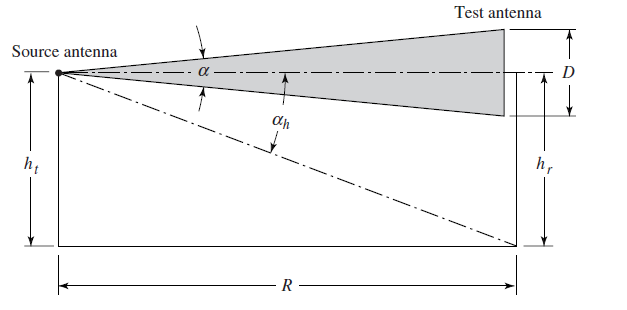
\includegraphics[scale=0.8]{arquitectura instalacion alcance elevado}
    \caption{Esquema de una instalación de alcance elevado extraído de \cite{Balanis_2016}}
    \label{Esquema de una instalación de alcance elevado}
\end{figure}

\newpage

En este tipo de instalaciones las contribuciones del entorno circundante generalmente se reducen o eliminan mediante:

\begin{enumerate}
    \item Una selección cuidadosa de la directividad y de los lóbulos secundarios de la antena de origen.

    \item El despejamiento de obstáculos que impidan tener una la línea de visión clara entre las antenas.

    \item La redirección o absorción de cualquier difracción o reflexión producida durante el proceso de medida.

    \item La utilización de técnicas especiales de procesamiento de señales como el etiquetado de modulación de la señal deseada o el uso de pulsos cortos.
\end{enumerate}

\subsubsection{Alcance inclinado}

Las instalaciones de alcance inclinado sitúan la antena bajo estudio junto con su posicionador en una torre de altura fija que no sea conductora mientras que la antena emisora se sitúa cerca del suelo como se refleja en la siguiente figura:

\begin{figure}[h] 
  \centering
    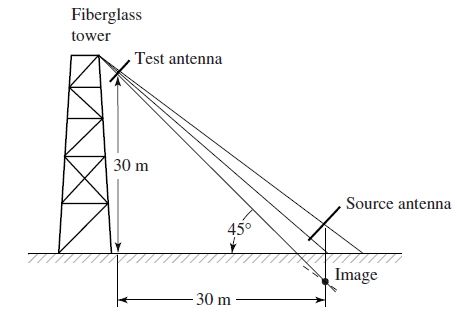
\includegraphics[scale=0.8]{arquitectura instalacion alcance inclinado}
    \caption{Esquema de una instalación de alcance inclinado extraído de \cite{Balanis_2016}}
    \label{Esquema de una instalación de alcance inclinado}
\end{figure}


De este modo, el máximo del patrón de radiación en espacio libre esté orientado hacia el centro de la antena de prueba. Dirigiendo de forma habitual el primer nulo del diagrama de radiación hacia el punto de reflexión estimado que se dará en el suelo para suprimir las señales reflejadas. Este tipo de instalaciones, por regla general, son más compactas que las de tipos elevados en el sentido de que requieren menos espacio para efectuar la medida. 

\newpage

 \subsubsection{Cámaras anecoicas}

Esta instalación proporciona un entorno controlado con una capacidad de simulación de cualquier tipo de clima a la par que proveen seguridad y minimizan radiación electromagnética procedente de fenómenos como la difracción. Las cámaras anecoicas se han desarrollado como una alternativa a las pruebas en exteriores, de forma que las medidas se realizan dentro de una cámara que tiene paredes cubiertas con absorbedores de radio frecuencia.\\

Actualmente, existen dos tipos básicos de diseños de cámaras anecoicas: la cámara rectangular y la cámara cónica. El diseño de cada una se basa en técnicas de óptica geométrica, y ambas intentan reducir o minimizar las reflexiones especulares. La siguiente figura muestra la configuración geométrica de cada una cámara:

\begin{figure}[h] 
  \centering
    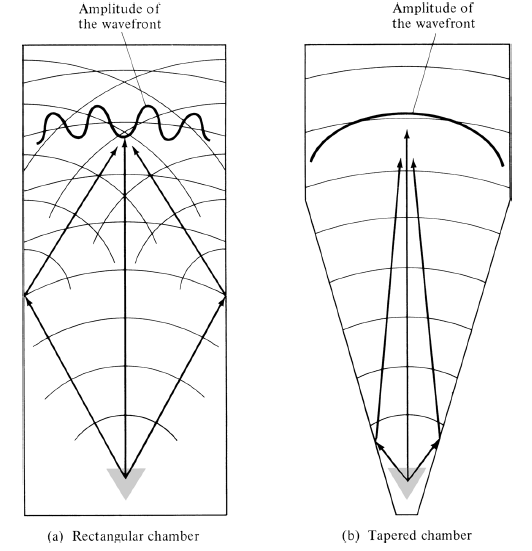
\includegraphics[scale=0.8]{geometría de las cámaras rectangular y cónica}
    \caption{Geometría de las cámaras rectangular y cónica extraido de \cite{Articulo_Kummer}}
    \label{Esquema de una instalación de alcance inclinado}
\end{figure}

La cámara rectangular suele estar diseñada para simular condiciones de espacio libre. El diseño toma en cuenta el patrón y la ubicación de la fuente, la frecuencia de operación, y asume que la antena receptora en el punto de prueba es isotrópica. La energía reflejada se minimiza mediante el uso de absorbentes de RF de alta calidad. A pesar del uso de material absorbente de RF, pueden ocurrir reflexiones especulares significativas, especialmente en ángulos de incidencia grandes.\\

\newpage

Las cámaras anecoicas cónicas tienen la forma de una bocina piramidal. Comienzan con una cámara cónica que conduce a una configuración rectangular en la región de prueba. En el extremo inferior de la banda de frecuencia para la cual la cámara está diseñada, la fuente generalmente se coloca cerca del vértice para que las reflexiones de las paredes laterales, que contribuyen a los campos de iluminación, se minimicen.\\


De entre los dos tipos de instalaciones existentes, este documento únicamente se va a centrar en las instalaciones de alcance en espacio libre. Dado que es el tipo de instalación más común y es sobre el que vamos a trabajar. En el siguiente capítulo encontraremos un análisis más profundo de este tipo de instalaciones, pero antes debemos presentar el método que nos va a permitir tomar medidas de campo lejano en este tipo de instalaciones.

\newpage

\subsection{Método de medida campo cercano a campo lejano}

La toma de medidas se puede reducir notablemente si efectuamos mediciones en campo cercano para luego usar métodos analíticos que nos permitan transformar estos datos calcular así el campo lejano. Este proceso se conoce como campo \textit{campo cercano-campo lejano} (NF/FF abreviado en inglés), y es la técnica empleada como norma general para medir el comportamiento de una antena y en la cual nos basaremos nosotros para efectuar nuestras transformaciones.\\

Este método se usa de forma habitual en cámaras anecoicas para poder realizar las mediciones en un ambiente controlado que proporciona una capacidad ideal para la medición. Sin embargo, como contrapartida, este método requiere de lo siguiente:

\begin{enumerate}
    \item Un sistema complejo que usualmente tiene un precio elevado.
    \item Un proceso de calibración complicado y extenso.
    \item Un software asociado al proceso de medida que debe ser muy sofisticado.
   \item  Una obtención de resultados que no es en tiempo real.
\end{enumerate}

\noindent
Las medidas en campo cercano, usualmente amplitud y fase, se obtienen mediante un escaneo del campo radiado sobre una superficie prefijada que típicamente es un plano, un cilindro o una esfera. La medida de estos datos es traspasada a campo lejano mediante la expresión analítica de la transformada de Fourier. La complejidad de este paso se hace aún mayor en el caso de pasar de una medición sobre una superficie plana a una cilíndrica, o de una cilíndrica a una esférica.\\

La elección del tipo de superficie suele tomarse en función de la antena que deseamos medir, teniendo las siguientes características:

\begin{itemize}
    \item El método de superficie plana es típico en el caso de medir antenas con gran ganancia. Especialmente los \textit{arrays} de fase plana, que requieren de menos carga computacional y no requieren reposicionar la antena.
    \item El método con superficie cilíndrica requiere de una mayor carga computacional comparado con la superficie plana, pero es útil en antenas donde interesa saber su rendimiento en función de la posición de la antena, además de ser el equipo de medida es el más barato de los tres.
    \item El método con superficie esférica es el más costoso en computación y en cuanto al equipo de medida. Da muy buenos resultados si medimos grandes sistemas de antenas. Este método es el que mejor se comporta con equipos de baja ganancia omnidireccionales.
\end{itemize}

\newpage

En un experimento basado en usar una superficie arbitraria, Morse y Feshbach mostraron en \cite{morse&Feshbach1953} que la elección del tipo de superficies es de hecho limitada dado que la derivación del vector de campo lejano a partir del campo cercano depende de que la función del vector de onda sea ortogonal a la superficie empleada. En base a esto, los seis sistemas de coordenadas válidos son el plano, el circular, el cilíndrico, el esférico, el cilíndrico elíptico, el cilíndrico parabólico y el cónico. Los tres primeros sistemas de coordenadas están orientados a la adquisición de datos, mientras que los tres últimos requieren pasar cilindros elípticos, cilindros parabólicos o esferas a coordenadas cónicas. Es por esto que las tres técnicas de campo cercano a campo lejano que se han desarrollado están basadas en ondas planas, cilíndricas o esféricas.\\

\begin{figure}[h] 
  \centering
    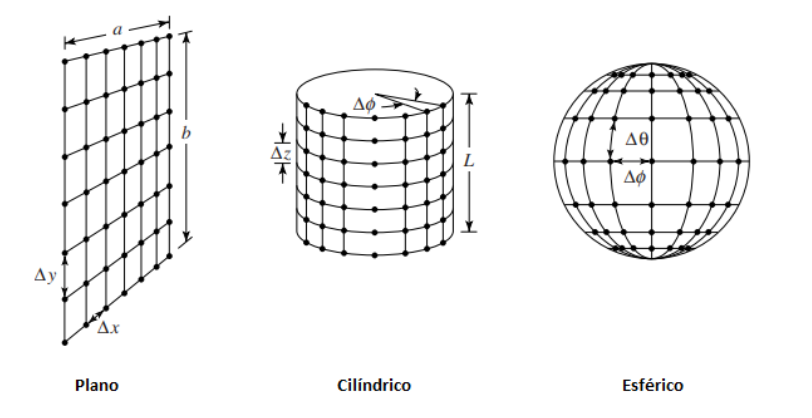
\includegraphics[scale=0.5]{sistemas de coordenadas}
    \caption{Sistemas de coordenadas empleados en el método de campo cercano a campo lejano}
    \label{Sistemas de coordenadas empleados en el método de campo cercano a campo lejano}
\end{figure}

La adquisición de datos de un campo cercano planar generalmente se realiza a través de una malla rectangular como la de la figura \ref{Sistemas de coordenadas empleados en el método de campo cercano a campo lejano}. En esta malla, el máximo espaciado de las muestras sigue la relación $\Delta x = \Delta y = \lambda/2$ . También es posible adquirir esta medida empleando una malla plana polar o una malla bipolar. En caso de usar una superficie plana, la antena bajo medida deberá estar estacionada mientras que la antena transmisora (usualmente una antena tipo bocina) se podrá mover a través de cualquier punto de la malla. Es fundamental tener en cuenta la directividad y polarización de nuestra antena transmisora, ya que esto debe tenerse en cuenta cuando empleemos técnicas de compensación.\\ 

Estos métodos de compensación de la antena transmisora emplean el teorema de reciprocidad de Lorentz para emparejar los campos lejanos de la antena a estudiar con los de la antena transmisora. La principal ventaja de la transformación de campo cercano a lejano planar sobre el cilíndrico o esférico es su simplicidad matemática.  Además, la transformación planar se puede sustituir aplicando computacionalmente la transformada de Fourier. Si asumimos que el número puntos es $2^n$, siendo $n$ positivo y entero, la transformada del campo completo planar puede obtenerse computacionalmente en un tiempo proporcional a: 

\begin{equation}
    t = (ka)2\log_2(ka)
    \label{proporcion temporal cálculo de fourier}
\end{equation}

\noindent
donde $a$ es el radio del círculo más pequeño descrito por la antena bajo estudio. La transformada planar está muy bien descrita para la medida de antenas con lóbulos traseros pequeños. Esto hace referencia a antenas de bocina, reflectores o arrays planos. 

\newpage

La principal ventaja de obtener los datos en campo cercano y extrapolar a campo lejano es que el patrón obtenido en campo lejano está limitado en pasos angulares. Esto implica que, si el escaneo de la superficie se hiciese con infinitos puntos, podríamos obtener computacionalmente un hemisferio del campo lejano sin ningún tipo de error. La medida por completo del campo lejano sobre superficies cilíndricas incluye además la información necesaria para, de forma computacional, obtener un patrón completo en azimut para todos los ángulos de elevación. Aunque esto no incluye ni a las regiones cónicas ni las tapas del propio cilindro.\\

En cuanto al uso de superficies esféricas, la información obtenida mediante el escaneo del campo lejano hace posible la predicción completa del patrón de radiación en campo lejano. Es decir, cualquier patrón de campo lejano puede ser computacionalmente obtenido a partir de la medida en campo cercado con un escaneo esférico. Otra ventaja añadida es que el escaneo esférico corrige típicamente la posición y orientación de la antena a medir y varía su orientación angular hacia la antena transmisora. Debido a que la antena transmisora siempre apunta directamente a la antena transmisora, la corrección de la antena transmisora puede ser pasar por alto si empleamos un escaneo con un campo lo suficientemente grande.\\

Pese a todo lo anterior, la principal desventaja del escaneo esférico radica en la transformada matemática. Una porción significativa de la transformada no puede realizarse a través de la FTT para lo cual empleamos integración numérica, operaciones con matrices y soluciones simultaneas de ecuaciones. Esto incrementa mucho la carga computacional y dificulta la transformación considerablemente con respecto al caso plano o cilíndrico.\\

\newpage

\section{Sobre las herramientas utilizadas}

Antes de entrar en profundidad en el contenido principal del documento, debemos comentar las herramientas principales que hemos utilizado durante el desarrollo del mismo.

\begin{itemize}
    \item \textbf{COMSOL}: Nos hemos apoyado en COMSOL como herramienta de simulación para poder construir y estudiar modelos de antenas. Gracias a este programa hemos podido generar conjuntos de datos que nos han permitido poner en práctica nuestras transformaciones y, de forma adicional, verificar que los resultados obtenidos coincidían con los proporcionados por la simulación.

    \item \textbf{Python}: Hemos utilizado Python como lenguaje de programación principal por sus muchas ventajas frente a otras opciones. Algunas de estas son disponer de librerías que nos faciliten mucho el trabajo a la hora de tratar con herramientas tales como la transformada de fourier, su flexibilidad a la hora de ejecutar el programa en cualquier sistema operativo, su comunidad activa y la velocidad en el desarrollo de los programas.

    \item \textbf{Wolfram Matematica}: Durante el desarrollo de las transformaciones necesitábamos disponer de otro conjunto de resultados que nos permitiese verificar los resultados de Python. Este hecho motivó el uso de Wolfram Matematica para desarrollar las transformaciones en este programa de forma paralela y así poder tener datos con los que comparar las transformaciones. La elecicón de este programa por encima de otros se debe a que ya dispone de muchas herramientas matemáticas necesarias para hacer la transformación como son las ecuaciones de Legendre o las de Hankel y su facilidad a la hora de programar ecuaciones complejas.
\end{itemize}

% 
\chapter{Análisis de las cámaras anecoicas}
\label{cha:Análisis de las cámaras anecoicas}

Como se intrdujo en el capítulo anterior, las cámaras anecoicas son instalaciones que se caracterizan por eliminar cualquier tipo de eco generado por una onda en su interior. Lo que hace que sean un entorno de medidas controlado y seguro que permite tomar medidas en su interior con una garantía absoluta de que no estarán contaminadas por interferencias electromagnéticas.\\

La motivación principal que impulsó la creación de estas cámaras es precisamente disponer de un entorno de medida aislado y perfectamente controlado. Dado que en un entorno abierto, las medidas se pueden contaminar por un considerablemente alto número de motivos. Entre ellos destacan la presencia de interferencias debidas a frentes de radiación externos y a las reflexiones procedentes de la antena transmisora. Además, las instalaciones abiertas están sometidas a condiciones atmosféricas que atenúan las medidas.\\

Debido a esto, el uso de la cámara anecoica se estableció como una alternativa superior a las medidas en el exterior no solo por poder eliminar las posibles interferencias, reflexiones, o por poder controlar condiciones atmosféricas que atenúan o fomenten la refracción, sino por su fiabilidad en las medidas y la facilidad con la que puede variarse la frecuencia de trabajo. De esta forma, se permite el poder caracterizar el comportamiento de una antena en un rango amplio de frecuencias de forma cómoda. Estableciendo la preferencia de este tipo de instalaciones para la medida de antenas en las que el patrón y ubicación de la fuente son factores clave. 

\newpage

\section{Límites de las cámaras anecoicas}

Para poder trabajar adecuadamente con una cámara anecoica necesitamos conocer previamente las limitaciones que presentan este tipo de instalaciones. Existen dos factores fundamentales a nivel físico que restringen el uso de la cámara anecoica y que vienen impuestos por construcción a los cuales vamos a dedicar los siguientes dos subapartados. Estos dos factores tienen que ver con la capacidad de absorción de la cámara y las dimensiones de la misma. 

\subsection{Límite del absorbente de radio frecuencia }

Como hemos comentado, la eliminación del eco de las cámaras anecoicas nos permite controlar el entorno de medida eliminando las reflexiones que pueda sufrir la onda plana. Sin embargo, no hemos comentado aún nada del elemento clave que nos permite asegurar esto, el absorbente de radio frecuencia. \\

El absorbente es un elemento fundamental de las cámaras anecoicas que cobra una importancia mayor en nuestro caso en particular. Esto se debe a que la cámara anecoica de la que disponemos es del tipo rectangular, que es el modelo de cámara que más favorece la convergencia de reflexiones en la antena receptora, lo que hace que sea la cámara más sensible al rendimiento del absorbente.
\\

Para que el absorbente cumpla con su propósito de forma correcta, debemos asegurar que la impedancia presente en el espacio libre y la impedancia del propio material absorbente tengan el mismo valor o uno muy próximo. Por ello es habitual que las cámaras tengan las paredes internas recubiertas con absorbente de RF en forma piramidal, ya que gracias a esta estructura, se logra que ambas impedancias sean idénticas. 

Sin embargo, el uso de un absorbente con forma piramidal tiene como inconveniente que el rendimiento del absorbente se deteriora conforme aumenta el ángulo de incidencia de la onda sobre él. Debido a esto, es imperativo conocer el ángulo de incidencia límite a partir del cual el absorbente es incapaz de eliminar los ecos de la onda y por tanto las medidas sufren la contaminación de ondas reflejadas.\\

Este valor suele venir definido en la hoja de características del fabricante, sin embargo, es interesante conocer la variación del ángulo de incidencia límite y la capacidad de absorción conforme varía la longitud de onda. Para ello vamos a hacer uso de una gráfica que ilustra una estimación del rendimiento de un absorbente piramidal sobre el que se aplica una onda de forma oblicua definida en el estándar 149-2021 \autocite{IEEEstd}.Esta es de especial interés en nuestro caso debido a que la incidencia presente en una cámara anecoica rectangular es precisamente de tipo oblicuo. 

\newpage

\begin{figure}
    \centering
    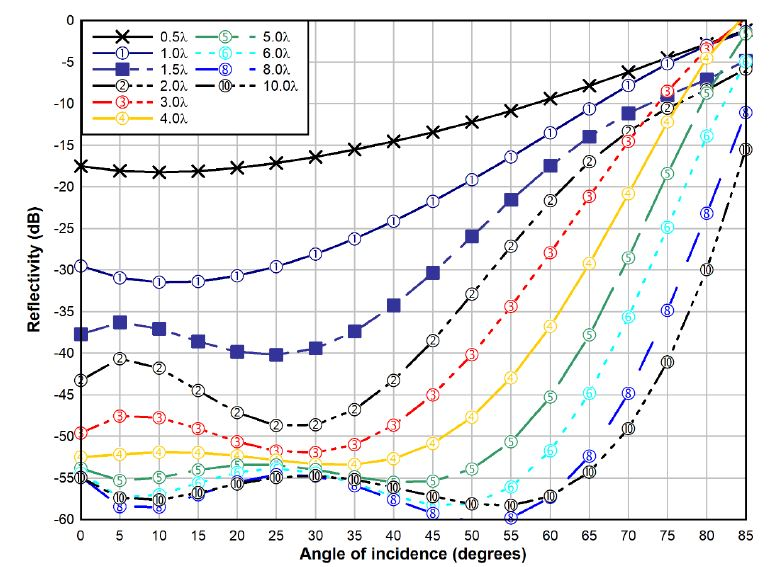
\includegraphics[scale=0.65]{Tabla-limite-angulo-incidencia}
    \caption{Curvas de la relación entre el ángulo de incidencia y la reflectividad}
    \label{Tabla-limite-angulo-incidencia}
\end{figure}

A partir de la gráfica de la figura \ref{Tabla-limite-angulo-incidencia} podemos llegar a una conclusión relativa a la longitud necesaria que debe medir nuestro absorbente. Estableciendo que, con la condición de que el absorbente sea más grande que la longitud de onda, podemos afirmar que el absorbente va a rendir correctamente y no vamos a tener ecos.
\\

Si aplicamos esta idea a un ejemplo práctico para hacernos una idea de lo que supone, significa que si empleamos una frecuencia de 150MHz perteneciente a la banda de la televisión necesitamos un absorbente que mida al menos 2 m de longitud. Estableciendo así la idea de que cuanto menor sea el tamaño de esta pirámide de absorbente, mayor será la frecuencia mínima a partir de la cual podemos efectuar mediciones sin tener efectos difractivos. 

\newpage

\subsection{Límite del tamaño de la cámara}

Al trabajar sobre una cámara anecoica rectangular, no solo debemos tener en cuenta el límite impuesto por el absorbente, sino también la longitud de la cámara. Esto se debe a que la longitud de la cámara nos va a limitar la longitud de onda mínima que podemos usar si queremos medir una antena de tamaño concreto en nuestra cámara y utilizar esas medidas como representativas del campo lejano.\\ 

Bajo esta premisa, urge conocer la distancia a partir de la cual podemos considerar las medidas del campo como medidas del campo lejano, la cual es fácilmente obtenible a partir de la siguiente expresión: 

                            \begin{equation}
                            R =\frac{2D^2}{\lambda}
                            \end{equation}
                       
Donde D es el tamaño de la apertura de nuestra antena y ${\lambda}$ es la longitud de onda en el vacío.\\
Esta expresión se puede reescribir de la siguiente forma si asumimos que el tamaño de la antena será de $n$ veces ${\lambda}$.

                            \begin{equation}
                            R =2n^2\lambda
                            \end{equation}

A partir de estas expresiones podemos obtener cual es la longitud de onda máxima que podemos emplear para medir nuestra antena si conocemos cuanto mide el largo de nuestra cámara anecoica rectangular. Así obtenemos el límite de trabajo de la cámara impuesto por el tamaño de la misma. 

\newpage

\subsection{Estudio de ambos límites combinados}

Una vez presentadas y explicadas ambas limitaciones, es interesante estudiar cómo se combinan entre si, dado que nos van a marcar la frecuencia mínima y máxima que podemos usar en una cámara. 
\\

Para ello, haremos uso de la gráfica vista en la figura \ref{Tabla-limite-angulo-incidencia}, de la cual extraemos el dato de que el absorbente piramidal de altura de $2\lambda$ debe proporcionar una atenuación de 40 dB en la reflexión. 
\\

A partir de esta reflectividad y definiendo $\theta$ como el ángulo de incidencia límite a partir del cual el rendimiento del absorbente decae, podemos obtener la distancia a partir de la cual cumplimos el requisito de campo lejano. Para encontrar dicha condición matemática, debemos aplicar relaciones trigonométricas. Motivo por el cual hemos representado el problema a resolver en la figura \ref{Geometría-del-ángulo-incidencia-absorvente} para facilitar las cosas. 

\begin{figure}[h]
    \centering
    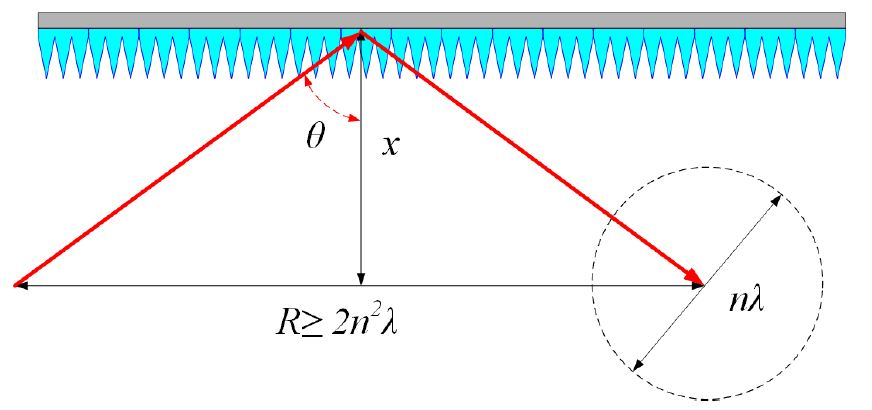
\includegraphics[scale=0.65]{Figura2-Geometria del angulo incidencia}
    \caption{Geometría del ángulo de incidencia en el absorbente de la cámara.}
    \label{Geometría-del-ángulo-incidencia-absorvente}
\end{figure}


Tras una serie de cálculos, somos capaces de obtener la siguiente expresión, que en un principio podría tomar cualquier valor: 

                        \begin{equation}
                        \tan\theta =\frac{R}{2x}
                        \end{equation}

\noindent
donde x es la distancia. 

\newpage

\section{Explicación de la toma de medidas}

Tras haber dedicado una sección a comprender el tipo de instalación que vamos a utilizar y las limitaciones que implica usarla, estamos a disposición de explicar cómo se efectúa la toma de medidas dentro de una instalación.\\

Durante el proceso de medida de una antena interactúan diversos sistemas de forma conjunta para poder caracterizar su comportamiento. La forma de trabajo de estos sistemas y su papel en la toma de medidas nos va a permitir hacernos una idea del proceso que nos permite caracterizar la antena bajo estudio. Debido a esto, esta sección se centra en comprender a alto nivel la arquitectura empleada en una cámara anecoica y cómo sus elementos nos permiten efectuar la toma de medidas .

\subsection{Arquitectura tipica de una cámara anecoica} 

En secciones anteriores hemos hecho referencia a la idea de que no todas las instalaciones son válidas para todos los tipos de antenas debido a que los requisitos necesarios para caracterizar una antena pasiva de un solo puerto son menos exigentes que los necesarios para medir una esfera de antenas de múltiples puertos usada en comunicaciones inalámbricas de alta velocidad. 
\\

Debido a esto y frente a la posibilidad de tener que construir una arquitectura totalmente nueva para cada tipo de antena, se decidió plantear un modelo general que podemos encontrar definido en el estándar 149-2021 \autocite{IEEEstd} y que toma la siguiente forma:

\begin{figure}[h]
    \centering
    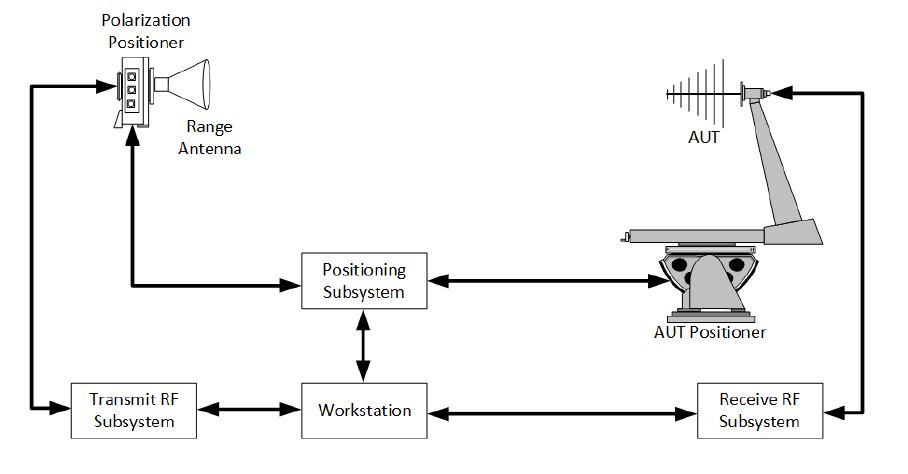
\includegraphics[scale=0.75]{Figura3-Modelo de una estacion completa de medidas}
    \caption{Esquema de una estación de medidas.}
    \label{Modelo-general-de-una-estación-de-medidas}
\end{figure}

\noindent
De todos los elementos presentes en esta arquitectura, nos vamos a centrar en dos de ellos, la antena transmisora y el subsistema de posicionamiento. Esto se debe a que nuestro objetivo no es detallar en profundidad cada subsistema, sino comprender todos los aspectos clave del proceso de medidas que necesitamos saber de cara a comprender las transformaciones.


\subsubsection{Sonda} 

Si nos fijamos en la figura \ref{Modelo-general-de-una-estación-de-medidas}, vemos la aparición de un elemento sobre el que debemos hablar antes de proseguir, la antena transmisora. Hasta ahora únicamente hemos hablado de que, idealmente, para caracterizar el campo lejano de una antena debemos radiar sobre ella una onda plana uniforme y del hecho de que en la realidad usamos ondas semejantes debido a que no es posible generar una onda plana ideal, pero no hemos comentamos nada relacionado con el emisor que usamos para transmitir dicha onda, el cual es precisamente el objeto de estudio de esta sección.
\\

El uso de esta antena transmisora, denominada sonda de ahora en adelante, es necesario para poder transmitir nuestra onda plana a la AUT para poder obtener medidas. Este hecho supone que en aras de poder conocer el comportamiento de la antena bajo test debemos conocer a la perfección el comportamiento de nuestra sonda, ya que de lo contrario no podremos discernir si las medidas son o no coherentes con respecto a lo enviado por la sonda.
\\

Otro concepto a destacar del uso de la sonda, es la idea de que nuestro sistema de medidas se basa en el uso de dos antenas, lo que da lugar a diferentes configuraciones posibles en función de donde se sitúan la sonda y la AUT. Debido a esto, existen diversas configuraciones en función de dónde estén situadas las antenas. Lo que da cámaras donde se pueden intercambiar de posición, otras donde las dos antenas están combinadas en un mismo instrumento y otras en las que ambas antenas están en posiciones fijas como la ilustrada en la figura \ref{Modelo-general-de-una-estación-de-medidas}. Pese a esto, independientemente de la configuración ante la que estemos, el funcionamiento de cada sistema es idéntico, por lo que todo lo visto a continuación es válido independientemente de dónde estén situadas las antenas. 

\subsubsection{Frecuencia de trabajo}

A excepción de algunas instalaciones especializadas en ciertos tipos de medida, es habitual que las instalaciones de medida se diseñen para usar un rango de frecuencia lo más amplio posible que cumpla los límites aceptables de funcionamiento presentados en secciones anteriores.\\

Pese a lo anterior, operar sobre un rango amplio de frecuencia trae consigo un problema principal relacionado con que usualmente el rango de frecuencias deseado excede el ancho de banda de trabajo de nuestra sonda. Razón por la cual es habitual disponer de una familia de antenas que en conjunto si permitan cubrir dicho rango de frecuencias. Este hecho implica la necesidad de disponer de un grupo de antenas que presenten una ganancia, ancho de haz y polarización coherentes con las medidas que queremos realizar nuestro rango, ya que no todas las antenas disponen de los mismos requisitos de línea de visión, reflexión o rangos compactos.\\

Otro aspecto a tener en cuenta es que necesitamos caracterizar la AUT en ambas polarizaciones, horizontal y vertical, lo que implica que necesitamos una forma de poder controlar la polarización usada en nuestra sonda. Empleándose usualmente sondas polarizadas de forma ortogonal o montando una sonda de polarización lineal sobre un posicionador de polarización que permita orientar el ángulo de inclinación de la polarización.


\subsubsection{Subsistema de posicionamiento} 

Para poder caracterizar una antena necesitamos tomar medidas del campo para los todos los ángulos de trabajo significativos, lo cual es posible gracias al subsistema de posicionamiento encargado de controlar la orientación de la sonda y la AUT durante el proceso de medida. Debido al hecho de que vamos a estar tratando con posiciones en el espacio, debemos apoyarnos en un sistema de coordenadas que nos permita asociar las medidas con la posición de las antenas, el cual típicamente es el sistema de coordenadas esférico. Al trabajar sobre este sistema de coordenadas, independientemente de si la línea de visión es fijas o móvil, dispondremos de dos ejes ortogonales que combinados permitan efectuar cortes en $\theta$ y $\phi$. Estos ejes se designan como el eje de rotación $\theta$ y el eje de rotación $\phi$. Los cuales están representados en la siguiente figura. 

\begin{figure}[h]
    \centering
    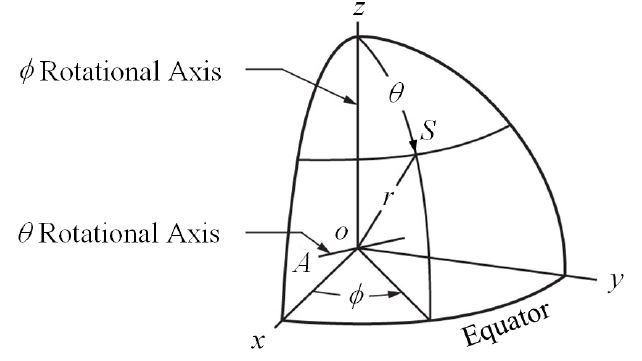
\includegraphics[scale=0.65]{Figura6-Ejes ortogonales para medir antenas}
    \caption{Ejes de rotación en un sistema esférico.}
    \label{Ejes-ortogonales-para-medir-antenas}
\end{figure} 

\noindent
En nuestro caso particular, la sonda está fija y haremos pivotar la AUT de forma que podamos tomar medidas en un rango significativo de ángulos.

\chapter{Transformaciones}
\label{cha:Transformaciones}

Una vez detallados todos los aspectos fundamentales relacionados con la caracterización de antenas, estamos a disposición de profundizar en nuestro objeto de estudio principal. El cual abordaremos siguiendo un camino natural que pasa por presentar y entender transformaciones sencillas que nos proporciones una base solida que nos permita dar el salto a la transformación de campo cercano a campo lejano en coordenadas esféricas.

\section{Definición del campo cercano y lejano}

Aunque en la introducción hablábamos de los términos de campo cercano y campo lejano, no dimos una definición formal de qué significaban, por lo que vamos a dedicar esta sección precisamente a esto. Una forma simple de entender el por qué se diferencia entre campo cercano y lejano consiste en estudiar el comportamiento de una onda conforme se aleja de la fuente que la provocó. Si estudiamos el comportamiento de una onda electromagnética, veríamos que conforme se aleja de la fuente que la generó más se asemeja a un frente de ondas plano hasta que llega a un punto donde directamente podemos aproximar que la onda tiene el mismo comportamiento que una onda plana.

\begin{figure}[h]
    \centering
    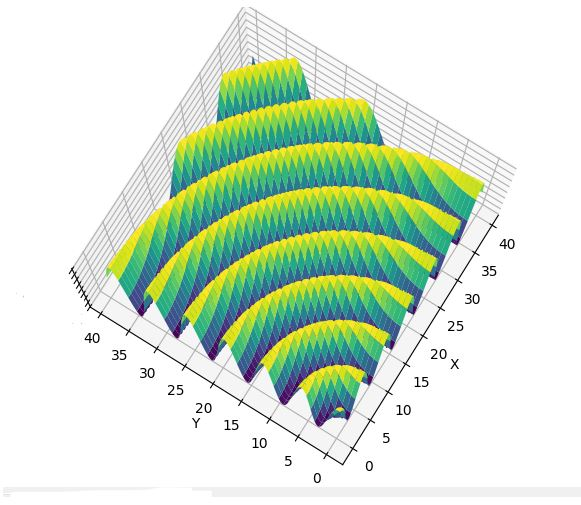
\includegraphics[scale=0.60]{Figura7-Esquema para ejemplificar el paso de onda esferica a onda plana}
    \caption{Representación visual del paso de onda esférica a onda plana}
    \label{Ejemplo-paso-onda-esferica-a-onda-plana}
\end{figure}

Precisamente es este punto en el cual la onda puede considerarse como onda plana donde se define la frontera entre campo cercano y campo lejano. De forma que los valores del campo donde aún no podemos aproximar que la onda tiene un comportamiento plano pertenecen al campo cercano, mientras que aquellos valores donde la onda se aproxima a una onda plana pertenecen al campo lejano.\\ 

En términos exactos, el campo lejano se define como la región en la que el frente de onda saliente de una antena es plano y la variación del patrón de radiación es independiente con respecto a la distancia de la propia antena. Por lo tanto, para considerar una onda perteneciente al campo lejano, su componente radial debe ser despreciable en comparación con la componente transversal y la relación entre el campo eléctrico y magnético debe ser igual a la impedancia intrínseca del medio. Debiéndose cumplir ambos requisitos en todas las direcciones angulares vistas desde la antena.
\\

Esto supone que para determinar la distancia a partir de la cual tenemos medidas pertenecientes al campo lejano hay que verificar estas propiedades para todas las direcciones angulares, cosa que ocurre a una distancia igual a:

\begin{equation}
                            R =\frac{2D^2}{\lambda}
\end{equation}

\noindent
donde D es la dimensión máxima de la antena y $\lambda$ es la longitud de onda de operación.\\

Si recordamos, esta fórmula ya la habíamos presentado al detallar las limitaciones presentes al usar una cámara anecoica. Lo que ilustra que, en realidad, todo el rato hemos tratado con la idea de campo lejano y campo cercano.
\newpage

\section{Transformación entre puntos del campo cercano}

La primera transformación que vamos a abordar para adquirir una base sólida de cara a afrontar las siguientes secciones consiste en transformar un punto de un plano $Z_1$ cualquiera perteneciente a la región de campo cercano a otro plano $Z_2$ perteneciente también a la región de campo cercano.

% Representaci ́on de los planos Z1 y Z_2 en perspectiva isometrica
\tdplotsetmaincoords{60}{125} % Establecer la perspectiva
\begin{figure}[htbp]
  \centering
  \begin{tikzpicture}[tdplot_main_coords,scale=2]
    % Plano Z1 en azul
    \fill[blue!20] (0,0,0) -- (2,0,0) -- (2,2,0) -- (0,2,0) -- cycle;
    \draw[blue] (0,0,0) -- (2,0,0) -- (2,2,0) -- (0,2,0) -- cycle;
    \node[blue] at (1,1,0) {\( Z_1 \)};
    % Plano Z2 en rojo
    \fill[red!20] (0,0,1) -- (2,0,1) -- (2,2,1) -- (0,2,1) -- cycle;
    \draw[red] (0,0,1) -- (2,0,1) -- (2,2,1) -- (0,2,1) -- cycle;
    \node[red] at (1,1,1) {\( Z_2 \)};
    % Ejes
    \draw[thick,->] (0,0,0) -- (2.5,0,0) node[anchor=north east]{\( x \)};
    \draw[thick,->] (0,0,0) -- (0,2.5,0) node[anchor=north west]{\( y \)};
    \draw[thick,->] (0,0,0) -- (0,0,1.5) node[anchor=south]{\( z \)};
  \end{tikzpicture}
  \caption{Representación de los planos \( Z_1 \) y \( Z_2 \) en perspectiva isométrica.}
  \label{fig:planos_NF_Z1_Z_2}
\end{figure}

Para ello, nos a basaremos en el manual de C.Balanis \autocite{Balanis_2016} para hacer un desarrollo previo que nos permita introducir de forma ordenada las ecuaciones fundamentales que debemos utilizar.
\\

Lo primero que debemos hacer es definir la expresión de un campo eléctrico genérico y de frecuencia $\omega$.

\begin{equation}
\vec{\tilde{E}}(\vec{r},t)=\vec{E}(\vec{r})\,e^{j\omega t}
\label{NFtoNF: eq-Campo E generico}
\end{equation}

Tras esto, debemos recordar la ecuación de onda del campo eléctrico, la cual tiene la siguiente forma:

\begin{equation}
\nabla^{2} \vec{\tilde{E}}(\vec{r},t)=\frac{1}{c}\frac{\partial^{2}
\vec{\tilde{E}}(\vec{r},t)}{\partial t^{2}}
\label{NFtoNF: eq-de-onde-campo-electrico}
\end{equation}

\noindent
donde $c$ representa la velocidad de propagación de la onda.\\

Desde esta expresión, podemos llegar a la ecuación de Helmholtz basándonos en \autocite{Pozar}.

\begin{equation}
(\nabla^{2}+k^{2})\vec{E}(\vec{r})=0
\label{NFtoNF: eq-Helmholtz}
\end{equation}

\noindent
con $k=\frac{\omega}{c}$

\newpage

Si ahora consideramos el campo $\vec{\tilde{E}}(\vec{r})$ como uno sobre el que podemos tomar medidas pertenecientes a un plano paralelo al eje $XY$ situado a una altura $z=z_{m}$ análogo a los planos vistos en la figura \ref{fig:planos_NF_Z1_Z_2}, entonces la función bidimensional $\vec{E}(x,y,z=z_{m})$ se puede representar
mediante una integral de Fourier de la siguiente forma:

\begin{equation}
\vec{E}(x,y,z=z_{m})=\int_{-\infty}^{\infty}\int_{-\infty}^{\infty}\vec{\hat{E}}(k_{x},k_{y},z=z_{m})
\,e^{-j (k_{x} x+k_{y} y)} dk_{x} dk_{y}
\label{NFtoNF: eq-fourier-campo-electrico}
\end{equation}

\noindent
expresión que podemos introducir en \eqref{NFtoNF: eq-Helmholtz}, obteniendo:

\begin{multline}
\left(\nabla^{2}+k^{2}\right)\left(\int_{-\infty}^{\infty}\int_{-\infty}^{\infty}\vec{\hat{E}}(k_{x},k_{y},z)
\,e^{-j (k_{x} x+k_{y} y)} dk_{x}
dk_{y}\right)=\\
\int_{-\infty}^{\infty}\int_{-\infty}^{\infty}\left(\nabla^{2}+k^{2}\right)\left[\vec{\hat{E}}(k_{x},k_{y},z)
\,e^{-j (k_{x} x+k_{y} y)}\right] dk_{x} dk_{y}=0
\label{NFtoNF: eq-fourier-campo-electrico-introducida-en-Helmholtz}
\end{multline}

\noindent
donde hemos devuelto la generalidad a la componente $z$ debido a que a efecto de los cálculos puede tomar cualquier valor. Hasta ahora era específica para reforzar la relación de esta componente con los planos de medida.
\\

Si ahora operamos el Laplaciano, obtenemos:

\begin{equation}
\int_{-\infty}^{\infty}\int_{-\infty}^{\infty}\left[\left(-k_{x}^{2}-k_{y}^{2}+k^{2}\right)+\frac{\partial^{2}}{\partial
z^{2}}\right]\left[\vec{\hat{E}}(k_{x},k_{y},z) \,e^{-j (k_{x}
x+k_{y} y)}\right] dk_{x} dk_{y}=0.
\label{NFtoNF: eq-fourier-campo-electrico-introducida-en-Helmholtz-con-laplaciano-operado}
\end{equation}

\noindent
como esta igualdad debe cumplirse para todos los valores de $x$ e $y$, el integrando ha de ser nulo. Lo que da como resultado:

\begin{equation}
\frac{\partial^{2}}{\partial
z^{2}}\vec{\hat{E}}(k_{x},k_{y},z)+w^{2}\vec{\hat{E}}(k_{x},k_{y},z)=0
\label{NFtoNF: resultado eq-fourier-campo-electrico-introducida-en-Helmholtz simplificada}
\end{equation}

\noindent
donde $w^{2}=k^{2}-k_{x}^{2}-k_{y}^{2}$.\\

A partir de esta expresión, podemos definir una solución general de \eqref{NFtoNF: resultado eq-fourier-campo-electrico-introducida-en-Helmholtz simplificada} de la siguiente forma:

\begin{equation}
\vec{\hat{E}}(k_{x},k_{y},z)=\vec{\mathcal{E}^{+}}(k_{x},k_{y})\,e^{-j
w z}+\vec{\mathcal{E}^{-}}(k_{x},k_{y})\,e^{j w z}
\label{NFtoNF: solucion eq-fourier-campo-electrico-en-Helmholtz-general}
\end{equation}

\noindent
donde el valor $\vec{\mathcal{E}^{+}}(k_{x},k_{y})\,e^{-j w z}$  representa una onda propagada en el sentido positivo del eje $z$, mientras que, como contrapartida, $\vec{\mathcal{E}^{-}}(k_{x},k_{y})\,e^{j w z}$ representa una onda propagada en dirección opuesta.\\


Para nuestro caso, solamente consideraremos la solución que contiene la onda $\vec{\mathcal{E}^{+}}(k_{x},k_{y})\,e^{-j w z}$, por lo que podemos reescribir la ecuación \eqref{NFtoNF: eq-fourier-campo-electrico} teniendo en cuenta solo esta solución. Obteniendo el mísmo resultado que el visto en la ecuación (12-73) en \autocite{Balanis_2016}.

\begin{equation}
\vec{E}(x,y,z)=\int_{-\infty}^{\infty}\int_{-\infty}^{\infty}\vec{\mathcal{E}^{+}}(k_{x},k_{y})
\,e^{-j (k_{x} x+k_{y} y+w  z)} dk_{x} dk_{y}
\label{NFtoNF:eq-fourier-balanis}
\end{equation}

\newpage

\subsection{Algoritmo para transformar el valor del campo cercano medido en $z=z_{1}$ en el campo cercano en otro plano $z=z_{2}$}
\label{sec:Algoritmo NFtoNF}


Partiendo del desarrollo hecho en la sección anterior, estamos a disposición de generar un algoritmo que nos permitirá calcular el campo eléctrico en una posición $z$ cualquiera que no tiene por qué ser la de salida de la onda. Es decir, no tiene por qué corresponderse con el plano radiante de la antena en el que hemos obtenido las medidas, sino que puede ser cualquier plano posterior. Esto significa que hablamos de un algoritmo capaz de calcular el campo cercano en un plano geométrico dado por una $z$ concreta a partir de los valores del campo medido en un plano anterior cualquiera independientemente de si este plano pertenece a la región de campo cercano o lejano. Esto es debido a que todo lo anterior es válido independientemente del valor de  $z$ a partir del cual consideramos que nuestro campo pasa a ser lejano.
\\

Lo primero que debemos hacer es estimar los modos dados por la función
$\vec{\hat{E}}(k_{x},k_{y},z=z_{1})$, para lo cual, hay que partir de la
ecuación \eqref{NFtoNF: eq-fourier-campo-electrico} e invertirla \footnote{En realidad, \eqref{NFtoNF:eq-fourier-campo-electrico-invertida} tiene la forma de
la transformada de Fourier directa de $\vec{E}(x,y,z=z_{1})$ como
función de $x$ e $y$, mientras que la ecuación \eqref{NFtoNF: eq-fourier-campo-electrico}
es formalmente la transformada inversa}, lo que nos da la siguiente ecuación:

\begin{equation}
\vec{\hat{E}}(k_{x},k_{y},z=z_{1})=\frac{1}{(2\pi)^{2}}\int_{-\infty}^{\infty}\int_{-\infty}^{\infty}\vec{E}(x,y,z=z_{1})
\,e^{j (k_{x} x+k_{y} y)} dx dy.
\label{NFtoNF:eq-fourier-campo-electrico-invertida}
\end{equation}

\noindent
No obstante, debido a que las medidas de las que partimos no son continuas, sino que conocemos el campo $\vec{E}(x,y,z=z_{1})$ en un conjunto de puntos
$(x,y)=(x_{n_{x}},y_{n_{y}})$ con $n_{x}=0,1,2,\ldots,N_{x}-1$ y
$n_{y}=0,1,2,\ldots,N_{y}-1$, deberemos discretizar nuestro problema teniendo en cuenta que en lugar de un plano continuo como el mostrado en la figura \ref{fig:planos_NF_Z1_Z_2} tendremos lo siguiente: 

\begin{figure}[h]
    \centering
    \begin{tikzpicture}[scale=1]
        \begin{axis}[
            xticklabels={,,},
            yticklabels={,,},
            zticklabels={$Z_{2}$, ,$Z_{1}$, ,$Z_{2}$},
            zlabel=$z$,
            xlabel=$x$,
            ylabel=$y$
            ]
            \addplot3[mesh] {5};
            \addplot3[mesh] {7};
        \end{axis}
    \end{tikzpicture}
    \caption{Representación de los planos $Z_{2}$ y $Z_{1}$ de forma discreta.}
    \label{fig:planos_NF_Z1_Z_2_discretos}
\end{figure}

\noindent
Debido a esto, deberemos discretizar \eqref{NFtoNF: eq-fourier-campo-electrico} y, por tanto,  \eqref{NFtoNF:eq-fourier-campo-electrico-invertida}, por lo que vamos a reescribirla de la siguiente forma:

\begin{equation}
\vec{\hat{E}}(k_{x},k_{y},z=z_{1})=\frac{\Delta x
\Delta y}{(2\pi)^{2}}
\sum_{n_{x}=0}^{N_{x}-1}\sum_{n_{y}=0}^{N_{y}-1}\vec{E}(x=n_{x}\Delta
x,y=n_{y} \Delta y,z=z_{1}) \,e^{j (k_{x} n_{x} \Delta x+k_{y} n_{y}
\Delta y)}
\label{NFtoNF:eq-fourier-campo-electrico-invertida-discretizada}
\end{equation}

\newpage

A partir de \eqref{NFtoNF:eq-fourier-campo-electrico-invertida-discretizada} se pueden obtener las componentes modales para cualquier valor de $(k_{x},k_{y})$. Con ellas se puede reconstruir el campo completo empleando la fórmula \eqref{NFtoNF: eq-fourier-campo-electrico}. De forma que, aparentemente, nos interesaría utilizar el mallado más fino posible en términos de $(k_{x},k_{y})$ para que la integral de \eqref{NFtoNF: eq-fourier-campo-electrico}, al aproximarse por su versión de sumatorio discreto, se calcule con el menor error posible. La malla original de los datos del campo eléctrico tiene una densidad de $N_{x} x N_{y}$ que condiciona la resolución real alcanzable en nuestra estimación.\\

Sin embargo, necesitamos tener en cuenta lo siguiente:
\begin{enumerate}
    \item No estamos teniendo en cuenta el teorema del muestreo dado que no por
    tomar más valores de $(k_{x},k_{y})$ vamos a tener una mejor descripción
    de $\vec{E}(x,y,z)$, sino que en realidad hay un nivel de información máximo
    asociado al muestreado en $(x,y)$.
    
    \item Afrontar el problema de esta forma no nos permite vincularlo con el algoritmo de la transformada rápida de Fourier (FFT), lo que nos impide beneficiarnos de las características fundamentales de este algoritmo.

\end{enumerate}

\noindent
Debido a esto, tenemos un especial interés en poder resolver nuestro problema con el algoritmo de la FFT ya que tanto la FFT como su inversa (IFFT) son algoritmos que tienen esto en cuenta. Llegados a este punto es interesante estudiar brevemente ambas expresiones, por lo que vamos a comenzar definiendo la expresión de la FFT. 

\begin{equation}
\vec{\hat{E}}_{m_{x},m_{y}}=\frac{1}{N_{x} N_{y}}
\sum_{n_{x}=0}^{N_{x}-1}\sum_{n_{y}=0}^{N_{y}-1}
\vec{E}(x=n_{x}\Delta x,y=n_{y} \Delta y,z=z_{1}) \,e^{j 2\pi
\frac{m_{x} n_{x}}{N_{x}}}\,e^{j 2\pi \frac{m_{y} n_{y}}{N_{y}}}
\label{NFtoNF:eq-fft1}
\end{equation}

\noindent
y a continuación la expresión de la IFFT.

\begin{equation}
\vec{E}_{n_{x},n_{y}}=
\sum_{n_{x}=0}^{N_{x}-1}\sum_{n_{y}=0}^{N_{y}-1}
\vec{\hat{E}}_{m_{x},m_{y}} \,e^{-j 2\pi \frac{m_{x}
n_{x}}{N_{x}}}\,e^{-j 2\pi \frac{m_{y} n_{y}}{N_{y}}}
\label{NFtoNF:eq-ifft1}
\end{equation}

Si compararamos  \eqref{NFtoNF:eq-fft1} con \eqref{NFtoNF:eq-ifft1}, vemos que para
poder aprovechar la herramienta que nos brinda la FFT debemos cumplir las siguientes igualdades:

\begin{subequations}
\begin{align}
k_{x}&= m_{x}\Delta k_{x}
\\
k_{y}&= m_{y}\Delta k_{y}
\\
\Delta x \Delta k_{x}&=\frac{2\pi}{N_{x}}
\\
\Delta y \Delta k_{y}&=\frac{2\pi}{N_{y}}.
\end{align}
\end{subequations}

\newpage

De todas ellas, las más relevantes para nosotros son las dos últimas debido a que son de obligado cumplimiento si queremos poder interpretar la ecuación \eqref{NFtoNF:eq-fourier-campo-electrico-invertida-discretizada} como
una FFT. Pudiendo definir\footnote{Si nos fijamos, $\Delta x$ y $\Delta y$ están
definidos por el muestreado del campo medido en $z_1$. Pero los de $\Delta k_{x}$ y $\Delta k_{y}$ aún no estaban definidos.} los valores de $\Delta k_{x}$ y
$\Delta k_{y}$ como:

\begin{align}
\Delta k_{x}&=\frac{2\pi}{\Delta x N_{x}}
\\
\Delta k_{y}&=\frac{2\pi}{\Delta y N_{y}}
\end{align}

Teniendo esto en cuenta, podemos definir la relación entre 
$\vec{\hat{E}}_{m_{x},m_{y}}$ de la ecuación \eqref{NFtoNF:eq-fft1} y 
$\vec{\hat{E}}(k_{x},k_{y},z=z_{1})$ de la ecuación \eqref{NFtoNF:eq-fourier-campo-electrico-invertida-discretizada} como:

\begin{equation}
\vec{\hat{E}}(k_{x}=m_{x} \Delta k_{x},k_{y}=m_{y} \Delta
k_{y},z=z_{1})= \Delta x \Delta y\vec{\hat{E}}_{m_{x},m_{y}}
\end{equation}

Expresión que, a nivel computacional, usaremos para calcular los modos $\vec{\hat{E}}(k_{x}=m_{x} \Delta k_{x},k_{y}=m_{y} \Delta
k_{y},z=z_{1})$ de la siguiente forma:

\begin{equation}
\vec{\hat{E}}_{m_{x},m_{y}}=\mbox{FFT}\{\vec{E}(x=n_{x}\Delta
x,y=n_{y} \Delta y,z=z_{1})\}.
\label{NFtoNF:eq-FFT-del-campo}
\end{equation}

Llegados a este punto, entramos en la segunda parte del proceso de transformación, donde haremos uso de la IFFT como herramienta para poder calcular el campo en $z=z_2$, para lo cual debemos discretizar \eqref{NFtoNF:eq-fourier-balanis} para poder aproximarnos a \eqref{NFtoNF:eq-ifft1} de la siguiente forma:

\begin{equation}
\vec{E}(x,y,z=z_{2}) =
\\
\Delta k_{x} \Delta k_{y}
\sum_{m_{x}=0}^{N_{x}-1}\sum_{m_{y}=0}^{N_{y}-1} 
\vec{\hat{E}}(k_{x},k_{y},z=z_{2})
\,e^{-j(n_{x}m_{x}\Delta x  \Delta k_{x} + n_{y}m_{y}\Delta xy  \Delta k_{y})}
\end{equation}

Haciendo uso de la ecuación \eqref{NFtoNF: solucion eq-fourier-campo-electrico-en-Helmholtz-general} y manteniendo que $\vec{\mathcal{E}^{-}}(k_{x},k_{y})=0$, entonces se cumple que:

\begin{equation}
\vec{\hat{E}}(k_{x},k_{y},z_{1})=\vec{\mathcal{E}^{+}}(k_{x},k_{y})\,e^{-j
w z_{1}}
\end{equation}

\noindent
expresión a partir de la cual podemos despejar $\vec{\mathcal{E}^{+}}(k_{x},k_{y})$ como:

\begin{equation}
\vec{\mathcal{E}^{+}}(k_{x},k_{y})=\vec{\hat{E}}(k_{x},k_{y},z_{1})\,e^{j
w z_{1}}
\label{NFtoNF:Ez2-cambio-fase}
\end{equation}

Lo que finalmente nos permite calcular el campo en $z=z_2$ como:

\begin{equation}
\vec{E}(x,y,z=z_{2})=\Delta k_{x} \Delta
k_{y}\,\mbox{IFFT}\{\vec{\hat{E}}(k_{x}=m_{x}\Delta
k_{x},k_{y}=m_{y} \Delta k_{y},z=z_{2})\}.
\label{NFtoNF:Ez2-final}
\end{equation}

\newpage

Finalmente, Conviene matizar las siguientes observaciones:
\begin{enumerate}
    \item Como el campo es vectorial, hay que aplicar separadamente este
    algoritmo a todas las componentes.
    \item Podemos trabajar con $\Delta x=\Delta y$.
    \item Los dos planos y las dos rejillas de medidas tienen que tener las mismas
    dimensiones pero pueden ser subdominios de áreas mayores en las
    cuales, por lo que sea, eliminamos ciertos márgenes. Eso ocurre en
    el caso de trabajar con medidas simuladas sobre espacios esféricos,
    donde los cortes con $z$'s dados no son iguales: nos quedamos con
    los subdominios de iguales dimensiones.
\end{enumerate}

\newpage
\subsection{Validación del algoritmo}

Una vez detallado el proceso teórico necesario para transformar las medidas del campo cercano, estamos a disposición de demostrar con un ejemplo que nuestra transformación es válida.\\
Para ello, vamos a realizar una simulación en COMSOL de una antena microstrip de la cual extraeremos los valores del campo cercano medido sobre un plano $Z_1$ que usaremos para calcular el campo cercano en un plano posterior $Z_2$.
\\

La antena microstrip que hemos construido en la simulación presenta las siguientes características básicas:

\begin{itemize}
    \item Tiene un punto de alimentación de $50\Omega$.
    \item La frecuencia de trabajo sera de 1.575 Ghz.
    \item Las dimensiones W y L de la antena son 7 mm y 15.5 mm.
\end{itemize}

\begin{figure}[h]
    \centering
    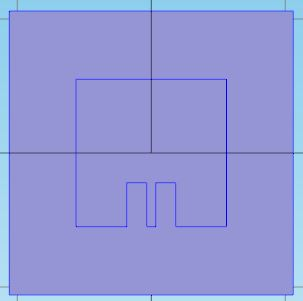
\includegraphics[scale=0.65]{Simulaciones COMSOL/MS-Planta de la antena}
    \caption{Esquemático de la antena microstrip en COMSOL.}
    \label{Simulaciones COMSOL/MS-Planta de la antena}
\end{figure}

\noindent

Correspondiéndole el siguiente diagrama de radiación:

\begin{figure}[h]
  \centering
    \includegraphics[scale=0.65]{Simulaciones COMSOL/MS-Diagrama de radiación}
    \caption{Diagrama de radiación de la antena simulada.}
    \label{MS-Diagrama de radiación de la antena simulada}
\end{figure}

\newpage

Una vez hecha la simulación, hemos desarrollado un programa en Python que implementa lo visto en \ref{sec:Algoritmo NFtoNF} utilizando los datos extraídos de la antena microstrip. No obstante, lo primero que debemos verificar es que estamos leyendo correctamente los datos extraídos de COMSOL, lo cual podemos hacer si enfrentamos la representación del campo a una distancia $Z_1$ devuelta por COMSOL con la obtenida en nuestro programa tras leer los datos.\\

En nuestro caso, vamos a tomar las medidas del campo medido sobre el plano $Z_1=15mm$ y las usaremos para obtener el campo en el plano $Z_2=30mm$, por lo que vamos a utilizar el módulo del campo en el plano $Z_1$ para la comprobación, que en la simulación tiene la siguiente forma:

\begin{figure}[h] 
  \centering
    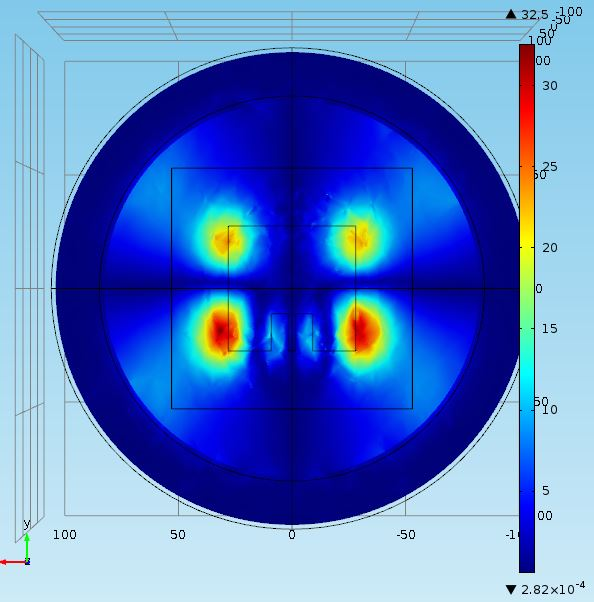
\includegraphics[scale=0.5]{Simulaciones COMSOL/MS-Enorm a 15mm}
    \caption{Módulo del campo medido en $Z_1=15mm$ en COMSOL.}
    \label{MS-Diagrama de radiación de la antena simulada}
\end{figure}

\newpage

Mientras que este mismo corte representamos desde nuestro programa a partir de los datos ledos de la simulación tiene la siguiente forma:

\begin{figure}[h] 
  \centering
    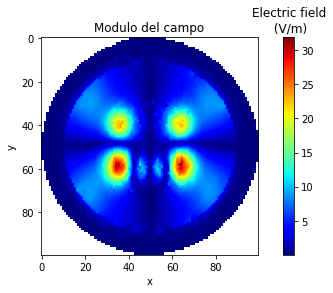
\includegraphics[scale=0.8]{Resultados python/MS-Enorm a 15mm python}
    \caption{Módulo del campo medido en $Z_1$ reconstruido en python.}
    \label{MS-Diagrama de radiación de la antena simulada}
\end{figure}

Como vemos, ambas representaciones coinciden, lo que confirma que tanto el programa como la simulación trabajan con los mismos datos, por lo que podemos realizar los cálculos que nos permiten calcular el campo en el plano posterior $Z_2$ y enfrentarlos a la simulación. Cabe destacar que el propósito de esta sección es únicamente demostrar que la transformación genera valores correctos. Debido a esto, nos vamos a centrar únicamente en los resultados y dejar la explicación del programa para el anexo correspondiente.\\

El primero de los resultados que vamos a estudiar es la representación bidimensional de la FFT de las componentes cartesianas del campo. 

\begin{figure}[h]
    \centering
    \begin{tikzpicture}
        % Inserta la imagen original
        \node[anchor=south west,inner sep=0] (image) at (0,0) {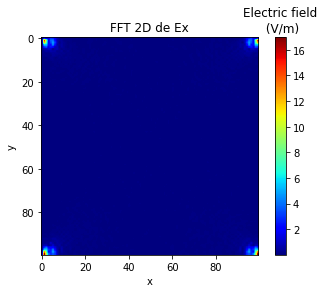
\includegraphics[scale=0.70]{Resultados python/MS-FFT 2D Ex a 15mm python.png}};

        % Dibuja un rectángulo en la esquina superior izquierda
        \begin{scope}[x={(image.south east)},y={(image.north west)}]
            \draw[red,thick] (0.1,0.7) rectangle (0.3,0.9); % Cambia los valores para ajustar la posición y tamaño del rectángulo
        \end{scope}
        
         % Inserta la imagen aumentada usando coordenadas específicas
        \node[anchor=south west] (zoomed) at (-4.5,0.4) {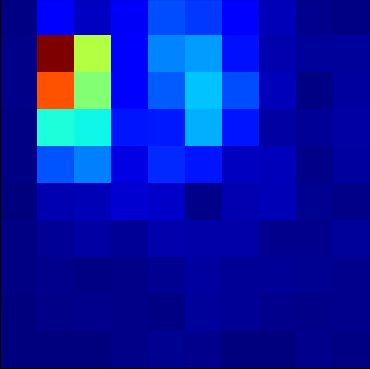
\includegraphics[scale=0.40]{Resultados python/MS-FFT 2D Ex a 15mm python ZOOM.png}};
        
                % Flecha roja
        \begin{scope}[x={(image.south east)},y={(image.north west)}]
            \draw[thick,->,red] (0.1,0.7) -- (-0.08,0.588);
        \end{scope}
        
    \end{tikzpicture}
    
    \caption{FFT 2D de la componente $E_x$ del campo en $Z_1$}
    \label{FFT 2D Ex a 15mm}
\end{figure}

\begin{figure}[h]
    \centering
    \begin{tikzpicture}
        % Inserta la imagen original
        \node[anchor=south west,inner sep=0] (image) at (0,0) {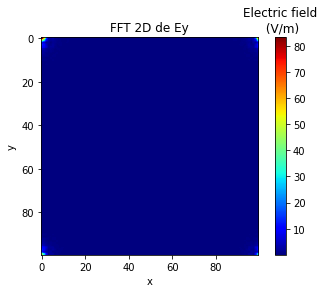
\includegraphics[scale=0.70]{Resultados python/MS-FFT 2D Ey a 15mm python.png}};

        % Dibuja un rectángulo en la esquina superior izquierda
        \begin{scope}[x={(image.south east)},y={(image.north west)}]
            \draw[red,thick] (0.1,0.7) rectangle (0.3,0.9); % Cambia los valores para ajustar la posición y tamaño del rectángulo
        \end{scope}
        
         % Inserta la imagen aumentada usando coordenadas específicas
        \node[anchor=south west] (zoomed) at (-4.5,0.4) {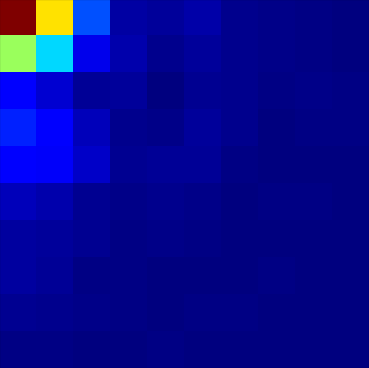
\includegraphics[scale=0.40]{Resultados python/MS-FFT 2D Ey a 15mm python ZOOM.png}};
        
                % Flecha roja
        \begin{scope}[x={(image.south east)},y={(image.north west)}]
            \draw[thick,->,red] (0.1,0.7) -- (-0.08,0.588);
        \end{scope}
        
    \end{tikzpicture}
    
    \caption{FFT 2D de la componente $E_y$ del campo en $Z_1$}
    \label{FFT 2D Ey a 15mm}
\end{figure}

\newpage

\begin{figure}[h]
    \centering
    \begin{tikzpicture}
        % Inserta la imagen original
        \node[anchor=south west,inner sep=0] (image) at (0,0) {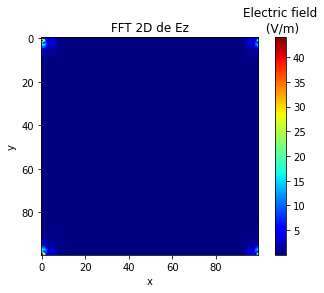
\includegraphics[scale=0.70]{Resultados python/MS-FFT 2D Ez a 15mm python.png}};

        % Dibuja un rectángulo en la esquina superior izquierda
        \begin{scope}[x={(image.south east)},y={(image.north west)}]
            \draw[red,thick] (0.1,0.7) rectangle (0.3,0.9); % Cambia los valores para ajustar la posición y tamaño del rectángulo
        \end{scope}
        
         % Inserta la imagen aumentada usando coordenadas específicas
        \node[anchor=south west] (zoomed) at (-4.5,0.4) {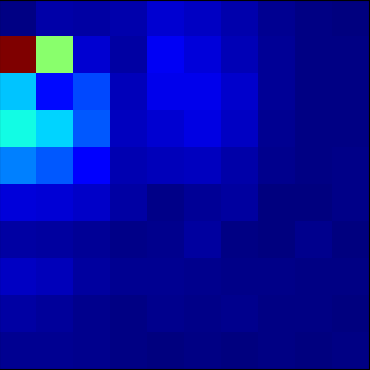
\includegraphics[scale=0.40]{Resultados python/MS-FFT 2D Ez a 15mm python ZOOM.png}};
        
                % Flecha roja
        \begin{scope}[x={(image.south east)},y={(image.north west)}]
            \draw[thick,->,red] (0.1,0.7) -- (-0.08,0.588);
        \end{scope}
        
    \end{tikzpicture}
    
    \caption{FFT 2D de la componente $E_z$ del campo en $Z_1$}
    \label{FFT 2D Ez a 15mm}
\end{figure}

Estas figuras corresponden al resultado de la ecuación \eqref{NFtoNF:eq-FFT-del-campo} y en ellas se muestran cuatro componentes modales situadas en las esquinas. 

\newpage

Partiendo de los resultados anteriores, debemos aplicar la IFFT tras haber aplicado previamente el cambio de fase tal y como veíamos en \eqref{NFtoNF:Ez2-final} y \eqref{NFtoNF:Ez2-cambio-fase}, lo que nos devuelve los siguientes resultados:

\begin{figure}[h] 
  \centering
    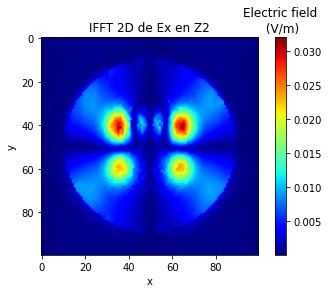
\includegraphics[scale=0.70]{Resultados python/MS-IFFT 2D Ex a 15mm python}
    \caption{IFFT 2D de la componente $E_x$ del campo en $Z_1$}
    \label{IFFT 2D Ex a 15mm}
\end{figure}

\begin{figure}[h] 
  \centering
    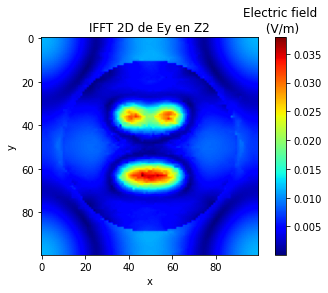
\includegraphics[scale=0.70]{Resultados python/MS-IFFT 2D Ey a 15mm python}
    \caption{IFFT 2D de la componente $E_y$ del campo en $Z_1$}
    \label{IFFT 2D Ex a 15mm}
\end{figure}
\newpage
\begin{figure}[h] 
  \centering
    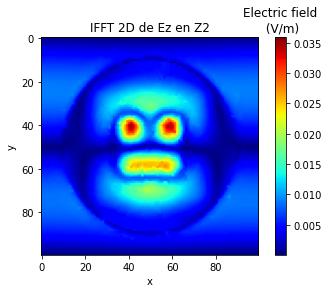
\includegraphics[scale=0.70]{Resultados python/MS-IFFT 2D Ez a 15mm python}
    \caption{IFFT 2D de la componente $E_z$ del campo en $Z_1$}
    \label{IFFT 2D Ex a 15mm}
\end{figure}

\newpage

A partir de los resultados de la IFFT podemos calcular finalmente el campo en el plano $Z_2=30mm$. Obtenido que su módulo en $Z_2$ tiene la siguiente forma:

\begin{figure}[h] 
  \centering
    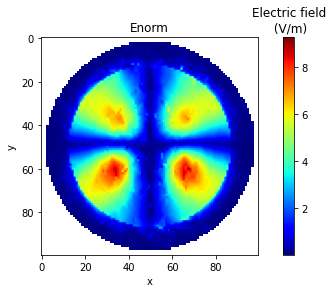
\includegraphics[scale=0.70]{Resultados python/MS-Enorm a 30mm python}
    \caption{Módulo del campo eléctrico en el plano $Z_2$}
    \label{IFFT 2D Ex a 15mm}
\end{figure}

De nuevo, para verificar que este resultado es válido vamos a enfrentar esta representación del modulo con la obtenida en la simulación de COMSOL. La cual tiene la siguiente forma:

\begin{figure}[h] 
  \centering
    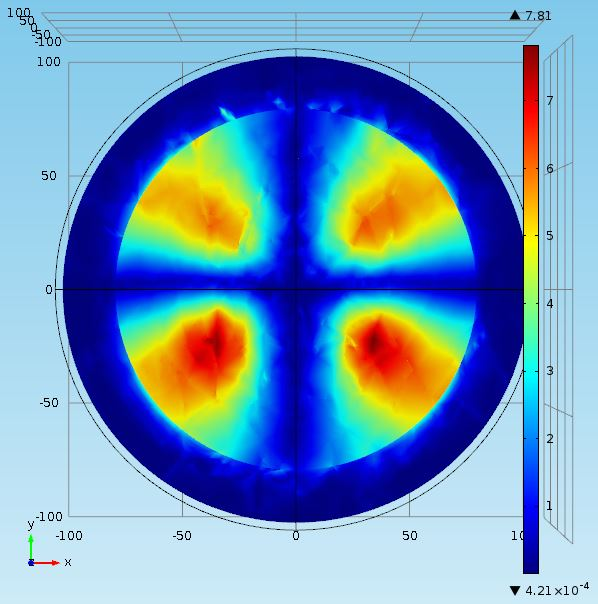
\includegraphics[scale=0.40]{Simulaciones COMSOL/MS-Enorm a 30mm}
    \caption{Módulo del campo medido en $Z_2$ en COMSOL.}
    \label{IFFT 2D Ex a 15mm}
\end{figure}

Si nos fijamos, las representaciones coinciden pero los valores máximos difieren ligeramente. Esto se debe a que la escala de COMSOL sitúa los colores rojos a partir de 6 $V/m$ y la librería de Python usada para representar el módulo los situa a partir de 7 $V/m$

\newpage

Una forma adicional de verificar los resultados pasa por restar los valores del módulo reconstruidos y simulados puesto que independientemente de la escala de color, la resta debería dar un campo prácticamente nulo como vemos que ocurre en la siguiente figura: 

\begin{figure}[h] 
  \centering
    \includegraphics[scale=0.70]{Resultados python/MS-Enorm comparación cuantitativa python}
    \caption{Comparación cuantitativa del campo simulado y calculado.}
    \label{IFFT 2D Ex a 15mm}
\end{figure}

En la figura \ref{IFFT 2D Ex a 15mm} podemos ver cómo la resta de los valores pertenecientes al campo se anulan dejando una región circular central a cero mientras que los valores externos a la circunferencia presentan patrones residuales que no tienen relación con el campo surgidos de los cálculos.

\newpage

\section{Transformación del campo cercano medido en una superficie plana a campo lejano en coordenadas esféricas}
\label{sec:validación NFtoNF esférico}
% //Esto es una demostración de lo visto en el punto anterior. NO es una transformación.

Una vez comprendido el proceso teórico que nos permite transformar medidas entre dos planos medidos en campo cercano y tras haber validado que transformación es correcta, debemos verificar que podemos obtener las medidas del campo cercano efectuadas sobre un plano en coordenadas cartesianas y calcular con ellas las medidas pertenecientes en una superficie esférica.\\

Lo primero que haremos será partir de la definición de un campo eléctrico cualquiera cuyos valores pertenecen al campo lejano.

\begin{equation}
\vec{E}(x,y,z)=\frac{jk_{z}}{2\pi r}\,e^{-jk_{0}r}{\vec{\mathcal{E}}}(k_{x}=k \sin\theta \cos\phi,k_{y}= k\sin\theta \sin\phi)
\label{NFtoFF:eq-campo-lejano}
\end{equation}

\noindent
donde $k_{x}$ y $ k_{y}$  contienen la información de los ángulos del sistema de referencia esférico que sirve de base para la expresión del diagrama de radiación en el campo lejano y  $k_{z}=k\cos\theta$. Siendo $k$ el número de onda en el vacío.\\

Para nuestra transformación, lo que realmente nos interesa es el valor del espectro, es decir, la función de modos ${\vec{\mathcal{E}}}(k_{x},k_{y})$. La cual responde a la siguiente expresión:

\begin{equation}
{\vec{\mathcal{E}}}(k_{x},k_{y})=\int_{-\infty}^{\infty}\int_{-\infty}^{\infty}\vec{E}(x,y,z=z_{0})\,e^{-j k_{x}x}\,e^{-jk_{y}y} dx dy.
\label{NFtoFF:eq-modos-del-campo-lejano}
\end{equation}
 
En la ecuación \eqref{NFtoFF:eq-modos-del-campo-lejano} podemos extraer una característica muy importante,  que la extracción de las componentes modales no depende del plano $z$, sino que puede tomar cualquier valor. Lo que significa que, mientras las medidas de dicho plano pertenezcan al campo cercano, la descomposición será siempre la misma.\\
Por otro lado, debemos tener en cuenta que en realidad solo conoceremos como es el campo  $\vec{E}(x,y,z=z_{0})$ en un conjunto discreto de puntos $(x,y) = (x_{n_{x}},y_{n_{y}})$ con  $n_{x}=0,1,2,\ldots,N_{x}-1$ y  $n_{y}=0,1,2,\ldots,N_{y}-1$. Debiendo reescribir nuestra ecuación de modos para que se ajuste a este conjunto de valores a la vez que adaptamos la ecuación para que podamos hacer uso de la transformada discreta de Fourier para poder hacer uso de la FFT.

Tras este razonamiento, vamos a reescribir la ecuación \eqref{NFtoFF:eq-modos-del-campo-lejano} de la siguiente forma: 
\begin{align}
{\vec{\mathcal{E}}}(k_{x},k_{y})&=\frac{L_{x}L_{y}N_{x}N_{y}}{4 \pi^2 (N_{x}-1)(N_{y}-1)} \nonumber \\
&\times \sum_{n_{x}=1}^{N_{x}-1}\sum_{n_{y}=1}^{N_{y}-1} DFT(\vec{E}(x=n_{x}\Delta
x,y=n_{y}\Delta
y,z=z_{0}))\,e^{-j k_{x}n_{x} \Delta x}\,e^{-jk_{y}n_{y} \Delta y}
\label{NFtoFF:eq-fourier}
\end{align}
\noindent
donde:

\begin{itemize}
    \item $N_{x}$ y $N_{y}$ son respectivamente el número de puntos del campo cercano en la dirección $x$ e $y$ .
    \item $L_{x}$ y $L_{y}$  es la longitud de la apertura en las dimensiones  $x$ e $y$.
\end{itemize}

\newpage

\noindent
De esta forma, la ecuación \eqref{NFtoFF:eq-fourier} corresponde a la descomposición modal del campo. Sin embargo, debemos discretizando los valores de $k_{x}$ y $k_{y}$ para poder aplicar la DFT aplicando las siguientes expresiones: 

\begin{subequations}
\begin{align}
k_{x}&= m_{x}\Delta k_{x}
\\
k_{y}&= m_{y}\Delta k_{y}
\\
\Delta x \Delta k_{x}&=\frac{2\pi}{N_{x}}
\\
\Delta y \Delta k_{y}&=\frac{2\pi}{N_{y}}.
\end{align}
\end{subequations}

Cabe destacar que podemos hacer este paso debido a que hay una definición implícita de $k_{x}$ y $k_{y}$ obtenida de la teoría de la DFT y de su valor como estimador espectral ya que necesitamos que la multiplicación de $\Delta x \Delta k_{x}$ sea igual a $\frac{2\pi}{N_{x}}$ para poder convertir la expresión en una sobre la cual poder hacer la DFT.\\

Si volvemos al contexto de nuestras medidas, nos damos cuenta que estamos trabajando precisamente con una malla regular de valores $k_{x}\times k_{y}$ correspondientes a coordenadas cartesianas del sistema de referencia del dominio transformado. Este hecho implica que a partir de esta malla, podemos dar una correspondencia entre los valores de $k_{x}$ y $k_{y}$ y los valores pertenecientes a una malla irregular en el dominio angular de dimensiones $\theta \times \phi$.\\

Discretizando entonces los valores de $k_{x}$ y $k_{y}$ de \eqref{NFtoFF:eq-fourier} obtenemos: 

\begin{equation}
{\vec{\mathcal{E}}}_{m_{x},m_{y}}=\frac{1}{N_{x} N_{y}}
\sum_{n_{x}=0}^{N_{x}-1}\sum_{n_{y}=0}^{N_{y}-1}
\vec{E}(x=n_{x}\Delta x,y=n_{y} \Delta y,z=z_{0}) \,e^{j 2\pi
\frac{m_{x} n_{x}}{N_{x}}}\,e^{j 2\pi \frac{m_{y} n_{y}}{N_{y}}}
\label{eq-fft1}
\end{equation}

Lo que finalmente nos permite reescribir \eqref{NFtoFF:eq-campo-lejano} introduciendo el uso de los ángulos $\theta \times \phi$:

\begin{align}
\vec{E}(r,\theta,\phi)&=\frac{jk_{z}}{2\pi r}\,e^{-jk_{0}}{{\vec{\mathcal{E}}}}(k_{x}=k \sin\theta \cos\phi,k_{y}= k\sin\theta \sin\phi)\nonumber
\\
\vec{E}(r,\theta_{m},\phi_{m})&=\frac{jk_{z}}{2\pi r}\,e^{-jk_{0}}{{\vec{\mathcal{E}}}}(k_{x}=m_{x}\Delta k_{x},k_{y}= m_{y}\Delta k_{y})=\frac{jk_{z}}{2\pi r}\,e^{-jk_{0}}{{\vec{\mathcal{E}}}}_{m_{x},m_{y}}\nonumber
\\
\label{eq-fourier3}
\end{align}

Pudiendo reconstruir el campo eléctrico para cualquier valor de $\theta$ y $\phi$ a partir de esta ecuación teniendo en cuenta que los valores de los ángulos $\theta \times \phi$ pueden corresponder a valores que no formen parte de nuestra malla $k_{x}\times k_{y}$. Debiendo interpolar estos ángulos con la malla de valores  $k_{x}\times k_{y}$  para poder obtener su valor correspondiente.
\\

\newpage

Finalmente, debemos matizar las siguientes observaciones:
\begin{enumerate}
\item Si efectuamos este cálculo sobre una antena bajo test, debemos saber que tiene una limitación ligada a cómo medimos físicamente la antena ya que solo será válido mientras respetemos ángulos de medidas menores a los siguientes:
\begin{equation}
\vartheta = \pm\arctan \frac{S-D}{2r_{0}}
\end{equation}
donde $S$ es la longitud del área de muestreo, $D$ es el diámetro de la antena bajo test y $r_ {0}$ es la distancia de separación entre la abertura de la antena bajo test y el plano de medida.
\end{enumerate}

\newpage

\subsection{Algoritmo para demostrar la validación}
Tras haber detallado el proceso teórico usado para demostrar que la transformación es válida, estamos a disposición de hacer una demostración práctica tal y como hicimos en el caso cartesiano. Para llevar a cabo esta demostración, vamos a apoyándonos de nuevo en la simulación de la antena microstript hecha en COMSOL para extrae la información del campo medido en un plano $Z_1$ cualquiera perteneciente a la región del campo cercano. En esta ocasión, partiremos de las medidas tomadas en un plano $Z_1 = 40mm$ para diferenciarnos del ejemplo anterior. 

\begin{figure}[h]
  \centering
    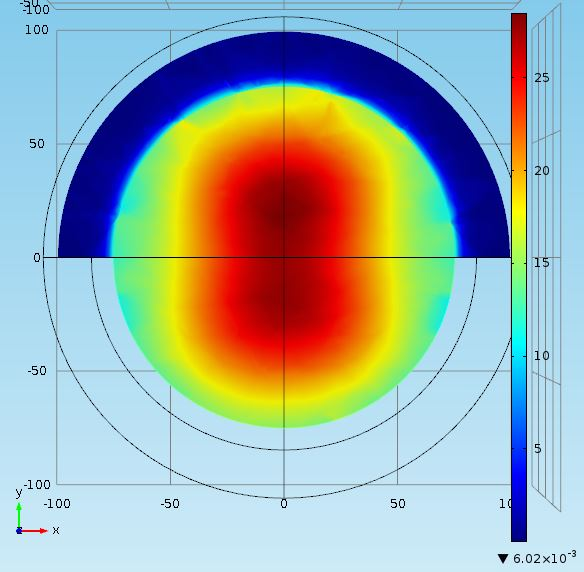
\includegraphics[scale=0.40]{Simulaciones COMSOL/MS-Enorm a 40mm}
    \caption{Módulo del campo eléctrico en $Z_1 = 40m$.}
    \label{MS-Modulo del campo eléctrico en Z_1}
\end{figure}

De nuevo, hemos desarrollado un programa en Python que implementa lo visto en la sección \ref{sec:validación NFtoNF esférico} partiendo de los datos extraidos de la antena microstrip simulada. Lo primero que debemos verificar es que hayamos hecho una lectura correcta de los datos tomados de COMSOL y verificar que coincide con lo visto en la figura \ref{MS-Modulo del campo eléctrico en Z_1}.

\begin{figure}[h]
  \centering
    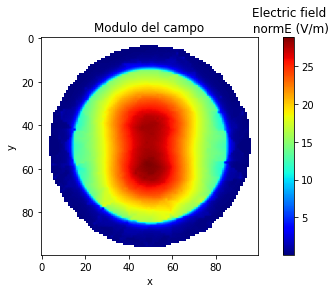
\includegraphics[scale=0.70]{Resultados python/MS-Enorm a 40mm Python}
    \caption{Módulo del campo eléctrico en $Z_1 = 40m$ reconstruido en python.}
    \label{MS-MS-Enorm a 40mm Python}
\end{figure}

Si confrontamos la figura \ref{MS-MS-Enorm a 40mm Python} con la figura \ref{MS-Modulo del campo eléctrico en Z_1} vemos que efectivamente las representaciones coinciden, confirmando de esta forma que los datos con los que vamos a tratar son exactamente iguales a los proporcionados por la simulación.\\

\newpage

Tras esta comprobación, y tras procesar los datos leídos pertenecientes al plano $Z_1$, estamos a disposición de emplear la FFT contando con que trabajamos con una malla regular de valores $k_{x}\times k_{y}$. Lo que supone que tendremos que dar una correspondencia entre los valores de nuestra malla y los valores pertenecientes al dominio angular de dimensiones $\theta \times \phi$.\\

Obteniendo los siguientes valores de la FFT para cada componente del campo eléctrico:

\begin{figure}[h]
  \centering
    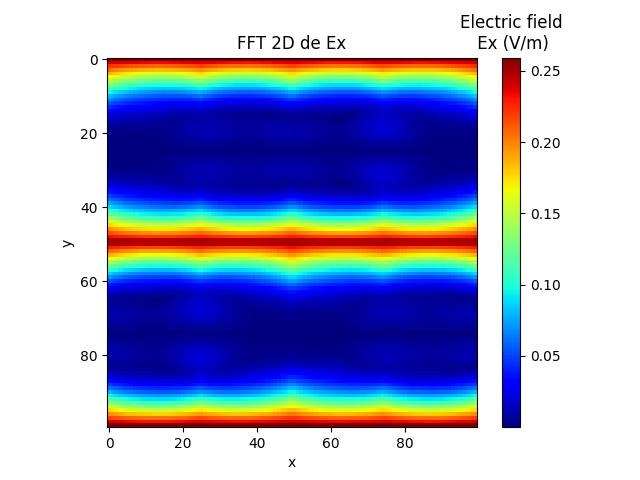
\includegraphics[scale=0.50]{Resultados python/MS- FFT 2D Ex}
    \caption{FFT 2D de la componente $Ex$ en $Z_2$}
    \label{MS- FFT 2D Ex}
\end{figure}

\begin{figure}[h]
  \centering
    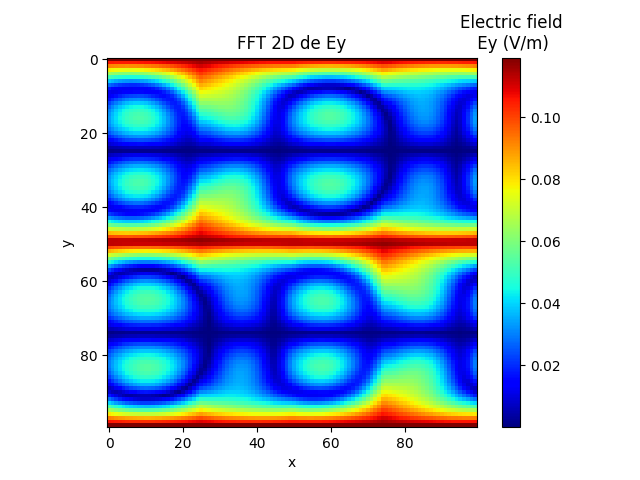
\includegraphics[scale=0.50]{Resultados python/MS- FFT 2D Ey}
    \caption{FFT 2D de la componente $Ey$ en $Z_2$}
    \label{MS- FFT 2D Ey}
\end{figure}

\newpage

\begin{figure}
  \centering
    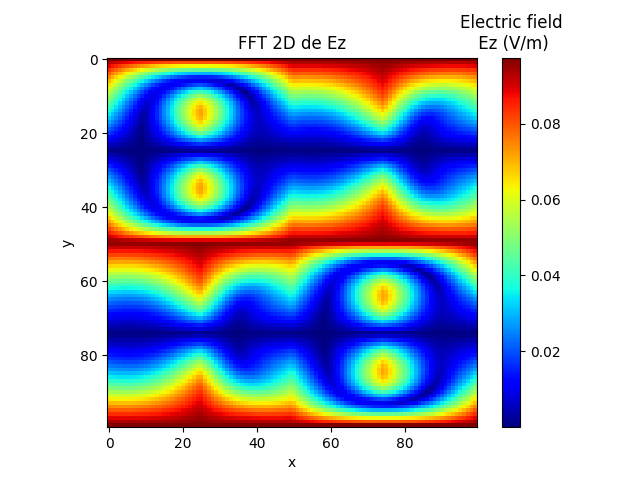
\includegraphics[scale=0.50]{Resultados python/MS- FFT 2D Ez}
    \caption{FFT 2D de la componente $Ez$ en $Z_2$}
    \label{MS- FFT 2D Ez}
\end{figure}

lo que nos da la siguiente representación del módulo del campo eléctrico medido en $Z_2=50mm$:

\begin{figure}[h]
  \centering
    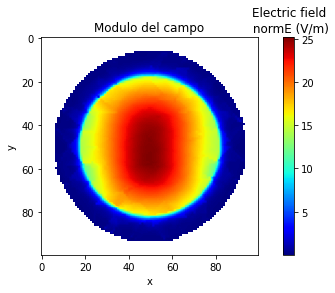
\includegraphics[scale=0.60]{Resultados python/MS-Enorm a 50mm Python}
    \caption{Módulo del campo eléctrico en $Z_2$ calculado en python}
    \label{MS-FFT 2D Ez}
\end{figure}

\newpage

El módulo del campo eléctrico del plano $Z_2$ simulado en COMSOL vemos que presenta una forma muy similar a la que obtenemos nosotros en la reconstrucción.

\begin{figure}[h]
  \centering
    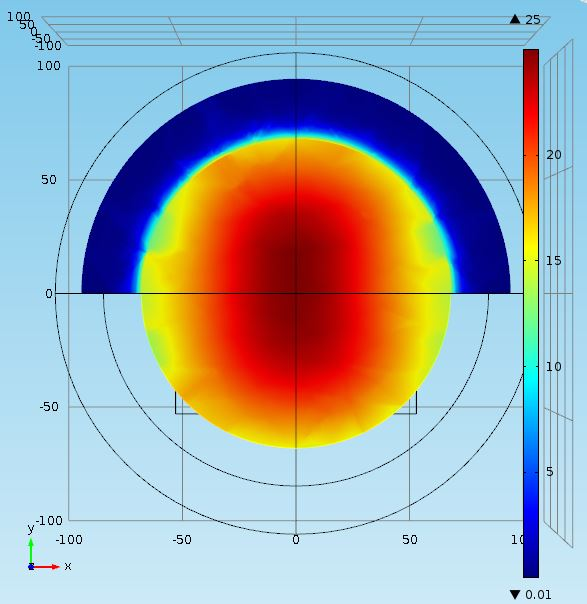
\includegraphics[scale=0.40]{Simulaciones COMSOL/MS-Enorm a 50mm}
    \caption{Módulo del campo eléctrico en $Z_2$ leído de COMSOL.}
    \label{MS-Enorm a 50mm}
\end{figure}

Una forma de comprobar esto es, de nuevo, hacer la resta entre el valor reconstruido y el proporcionado por la simulación, lo cual debería darnos una región central con valores nulos tal y como ocurre en la siguiente figura:

\begin{figure}[h]
  \centering
    \includegraphics[scale=0.60]{Resultados python/MS-Enorm comparación cuantitativa python NFtoFF}
    \caption{Comparación cuantitativa del campo simulado y calculado en coordenadas esféricas}
    \label{Comparación cuantitativa del campo simulado y calculado en coordenadas esféricas}
\end{figure}

\newpage

\section{Transformación del campo lejano a partir del campo cercano medido
en coordenadas esféricas}

Tras detallar las transformaciones anteriores, estamos a disposición de abordar el proceso que nos permite obtener el campo lejano a partir de medidas pertenecientes a campo cercano en coordenadas esféricas. Estableciendo como origen del sistema de coordenadas la propia antena que vamos a caracterizar. El uso de coordenadas esféricas implica que vamos a tratar con ecuaciones de ondas esféricas, que son objetos matemáticos de cierta complejidad. Debido a esto, lo primero que debemos hacer es introducir almenos los conceptos fundamentales de estas ecuaciones.

\subsection{Fundamentos necesarios de las ecuaciones esféricas}

Afrontar un problema que emplea a un sistema de coordenadas curvilíneo implica que el uso de ecuaciones diferenciales presenta dificultades añadidas. Para poder reducir parte de la complejidad, vamos a apoyarnos en una característica de las ecuaciones esféricas que nos permite resolver ecuaciones diferenciales aplicadas sobre un vector (en nuestro caso, el campo eléctrico) si consideramos que podemos construir dicho vector a partir dos vectores parciales.\\

Esta propiedad solo puede aplicarse en caso de que estos vectores parciales sean derivables a partir de una función puramente escalar que satisfaga las ecuaciones de onda vectoriales.
En nuestro caso, siempre vamos a tratar con vectores que pueden descomponerse en vectores parciales como demostraremos en el siguiente punto. Por el momento, nos basta con saber que ciertos vectores pueden ser descompuestos en otros parciales y que este caso particular es el que nos interesa estudiar.

\subsection{Ecuaciones de onda vectoriales}

Como hemos dicho, la condición fundamental que permite que podamos hacer u uso de vectores parciales es que dichos vectores cumplan las ecuaciones de onda vectoriales. Motivo por el cual vamos a dedicar esta sección a presentar estas ecuaciones. No obstante, las ecuaciones de onda vectoriales son, por si mismas, un objeto de estudio en si mismo, por lo que nos centraremos únicamente en los aspectos fundamentales que son relevantes para nuestro caso de uso particular y haremos ciertas simplificaciones que iremos detallando y justificando sobre la marcha.\\

En este punto es fundamental recordar que nosotros vamos a hacer uso de una cámara anecoica para la toma de medidas que nos asegura tener un entorno de medición con unas condiciones prácticamente iguales a las del vacío. Esto significa que disponemos de un dominio cerrado, es decir, un conjunto que incluye todos sus puntos incluidos los puntos límite y cuyo complemento es un conjunto abierto el cual además es un medio de propagación isotrópico sin fuentes.\\

Este entorno en particular resulta ser el más favorable a la hora de tratar con ecuaciones de onda vectoriales ya que todos los vectores de campo ($\vec{E}$,$\vec{B}$,$\vec{D}$ y $\vec{H}$),  el vector potencial $A$ o  los vectores de potencia de Hertz satisfacen una única ecuación diferencial que se cumple para todos ellos; y que toma la siguiente forma:

\newpage

\begin{equation}
\nabla^2C - \mu\varepsilon\frac{\partial^2C}{\partial^2{t}} - \mu\sigma\frac{\partial C}{\partial{t}} = 0\
\label{eq-esfvec-general}
\end{equation}

\noindent
donde $C$ representa cualquiera de los posibles vectores citados anteriormente.\\

Partiendo entonces de esta ecuación general, lo primero que vamos a hacer es emplear la propiedad de que las ecuaciones de onda esférica son lineales. Lo que nos nos permite simplificar la implicación del tiempo de nuestra ecuación debido a que gracias a la linealidad podemos reconstruir aquellos vectores que tengan una variación arbitraria con el tiempo a partir de soluciones armónicas. Pudiendo de esta forma reescribir la ecuación \eqref{eq-esfvec-general} sin perder con ello la generalización presente en expresión. \\

Esto implica que podemos afirmar que nuestro vector $C$ únicamente varía con respecto al tiempo en base al factor $e^{-jwt}$. Hecho que nos permite simplificar aún más nuestra expresión si recordamos que el operador laplaciano ($\nabla^2$) aplicado sobre un vector cualquiera equivale a:
\begin{equation}
\nabla^2C =\nabla(\nabla \cdot C) - \nabla\times\nabla\times C + k^2C
\label{eq-nabla-sobre-vector}
\end{equation}

\noindent
con $k^2$ = $\mu\varepsilon w^2 + j\mu\sigma w$ .\\

\noindent
Si aplicamos todo lo anterior, podemos entonces reescribir  \eqref{eq-nabla-sobre-vector} de la siguiente forma:
\begin{equation}
\nabla(\nabla \cdot C) - \nabla \times \nabla \times C + k^2 C = 0
\label{eq-esfvec-simplificada}
\end{equation}

\noindent
Una vez hemos llegado a la ecuación \eqref{eq-esfvec-simplificada}, disponemos de dos alternativa para trabajar con ella: 

\begin{enumerate}
    \item Podemos resolver \eqref{eq-esfvec-simplificada} como un sistema de tres ecuaciones escalares.
    \item Podemos simplificar la resolución de \eqref{eq-esfvec-simplificada} resolviendo tan solo tres ecuaciones escalares independientes si y solo si podemos obtener $C$ a partir de sus componentes rectangulares.
\end{enumerate}

De estos dos métodos, siempre vamos a preferir el segundo debido a que la resolución del sistema de ecuaciones implica una alta complejidad en los cálculos. Lo cual es especialmente desfavorable si lo comparamos con la resolución de las tres ecuaciones independientes. En nuestro caso particular podemos aplicar el segundo método debido a que siempre vamos a ser capaces de obtener el campo medido a partir de sus componentes rectangulares ya que nuestras medidas siempre van a cumplir las propiedades de ortogonalidad.
\\

Teniendo en cuenta todo lo anterior, podemos reescribir \eqref{eq-esfvec-simplificada} de la siguiente manera:

\begin{equation}
\nabla^2C_{j} + k^2C_{j} = 0
\label{eq-nabla-cuadrado-coordenada}
\end{equation}

donde $C_{j}$ hace referencia las componentes ($x$,$y$,$z$) del vector $C$.
\\

\newpage

Este hecho implica que tendremos tantas soluciones de \eqref{eq-nabla-cuadrado-coordenada} como vectores $C$ existan, por lo que de ahora en adelante vamos a considerar $\psi$ como una función escalar cualquiera que es solución de \eqref{eq-nabla-cuadrado-coordenada} para representar dicha generalidad:

\begin{equation}
\nabla^2\psi + k^2\psi = 0
\label{eq-nabla-cuadrado-coordenada-con-una-soculicon-por-vector-C}
\end{equation}

De esta forma; y considerando $\vec{a}$ como un vector unitario constante cualquiera, podemos escribir tres vectores independientes a partir de $\psi$ que son, de hecho, solución de \eqref{eq-esfvec-simplificada}:
\begin{subequations}
\begin{align}
    \vec{L}&= \nabla\psi \label{eq:Lirrotacional}\\
    \vec{M}&= \nabla\times a\psi\\
    \vec{N}&=\frac{1}{k}\nabla\times N
\end{align}
\end{subequations}

Estas tres ecuaciones presentan ciertas propiedades que merece la pena destacar. De entrada, gracias a ser $\vec{a}$ un vector unitario, podemos reescribir $\vec{M}$ de la siguiente manera:    

\begin{equation}
\vec{M}= \vec{L} \times a = \frac{1}{k}\nabla \times \vec{N}
\label{eq-M-reescrito}
\end{equation}


Por otro lado, el vector $\vec{M}$ es perpendicular a $\vec{L}$ para nuestra posible solución $\psi$, lo que significa que $L\cdot M=0$.Mientras que, por definición, $\vec{L}$ cumple las siguientes dos propiedades:
\begin{align}
    \nabla  \times \vec{L} &=0 \\
    \nabla  \cdot \vec{L}  &=\nabla^2\psi = -k^2 \psi
\end{align}

\noindent
donde hemos aplicado la ecuación \eqref{eq:Lirrotacional} para obtener el carácter rotacional del vector $\vec{L}$ y convertir su divergencia en un laplaciano.\\

Si además de lo anterior tenemos en cuenta que $\vec{M}$ y $\vec{N}$ son vectores de campo eléctrico en nuestro caso particular, significa que tanto $\vec{M}$ como $N$ son capaces de crear un campo magnético, por lo que, como pertenecen a un dominio que podemos considerar prácticamente igual al vacío, sus divergencias son nulas para cualquier punto dentro de él, o lo que es lo mismo, los vectores $\vec{M}$ y $N$ cumplen la condición de campo solenoidal:
\begin{align}
    \nabla\cdot \vec{M} &= 0
    \label{M-cumplen-ser-campo-solenoidal}\\
    \nabla\cdot \vec{N} &= 0
    \label{N-cumplen-ser-campo-solenoidal}
\end{align}

\newpage

Una vez presentadas todas estas propiedades de los vectores $\vec{L}$, $\vec{M}$ y $\vec{N}$, hay que tener en cuenta que existen tres tipos de soluciones para una ecuación diferencial, la general, la particular y la singular.\\
En nuestro caso concreto, podemos asumir que para cada punto existe una única solución $C$ correspondiente al valor del campo eléctrico en dicho punto. Lo que significa que vamos a manejar las soluciones particulares de \eqref{eq-nabla-cuadrado-coordenada-con-una-soculicon-por-vector-C}.\\

Para ilustrar esto, de ahora en adelante vamos a hacer uso de la notación $\psi_{n}$ para hacer referencia a cualquiera de estas soluciones particulares de la ecuación diferencial. De forma que para cada solución $\psi_{n}$ existe un conjunto de vectores $L_{n}$, $M_{n}$ y $N_{n}$. Es importante diferenciar esta generalidad de la anterior, ya que ahora no nos estamos refiriendo a una ecuación general $\psi$ sino a $\psi_{n}$ soluciones de ecuaciones que podemos obtener debido a que cumplen con los puntos anteriores que nos permiten asumir que existe una única solución para cada punto obtenible a partir de sus vectores $L_{n}$, $M_{n}$ y $N_{n}$.
\\

De los tres vectores $L_{n}$, $M_{n}$ y $N_{n}$ solo vamos a trabajar con $M_{n}$ y $N_{n}$ debido a que a cuando tratamos con una función solenoidal, es decir, una función cuya divergencia es nula en todo el dominio de puntos en la que existe dicha función, su extensión se puede obtener únicamente en términos de  $M_{n}$ y $N_{n}$.\\
Lo que supone que a partir de los vectores parciales $M_{n}$ y $N_{n}$ podemos obtener el valor del campo.\\

\noindent
Todo esto significa que si se cumple que:
\begin{enumerate}
    \item Que la variación arbitraria del tiempo entra en juego únicamente como un factor armónico $e^{-jwt}$.
    \item Que estamos trabajamos con un medio donde la densidad de cargas libres es nulo en todas partes.
    \item   Que nuestro medio es isotropico.
    \item Podemos caracterizar la conductividad de nuestro medio de forma única con valor $\sigma$.

\end{enumerate}

\noindent
entonces podemos definir los campos $E$ y $H$ de esta forma:

\begin{equation}
\vec{E} = \frac{jw\mu}{k^2}\nabla \times \vec{H}\xrightarrow{}   \vec{H}= \frac{1}{jw\mu}\nabla \times \vec{E}
\label{campo-EyH-cumpliendo-simplificacion-con-MnyNn}
\end{equation}

Si suponemos además que el vector potencial también puede ser representado por una expansión de funciones vectoriales características, entonces podemos escribir el valor del vector potencial como:

\begin{equation}
\vec{A} = \frac{1}{w}\sum_{n}(a_{n}M_{n}+b_{n}N_{n}+c_{n}L_{n})
\label{vector-potencial-cumpliendo-simplificacion-con-MnyNn}
\end{equation}

\noindent
donde los coeficientes $a_{n}, b_{n}, c_{n}$ pueden ser obtenidos a partir de la distribución de carga del campo.\\

Siendo en este punto donde vamos a aplicar las propiedades de $L_{n}$, $M_{n}$ y $N_{n}$ mencionadas anteriormente para poder ignorar el vector $L_{n}$. De manera que haciendo uso de la relación $\mu H = \nabla \times A$ podemos escribir las ecuaciones de campo como:


    \begin{equation}
        \vec{E} = - \sum_{n}(a_{n}M_{n}+b_{n}N_{n})
    \label{eq-E general usando Mn y Nn}
    \end{equation}

    \begin{equation}
         \vec{H} = - \frac{k}{jw\mu}\sum_{n}(a_{n}M_{n}+b_{n}N_{n})
    \label{eq-H general usando Mn y Nn}
    \end{equation}  

\newpage

A partir de \eqref{eq-E general usando Mn y Nn} somos capaces de expresar nuestro campo eléctrico en función de las ecuaciones de onda esférica $M_{n}$ y$N_{n}$ y los coeficientes de onda $a_{n}$ y $b_{n}$. Pudiendo entonces definir una expresión que obtenga el campo eléctrico para cualquier valor de $r$, $\theta$ y $\phi$ de la siguiente forma:
\begin{equation}
\vec{E}(r,\theta,\phi)=\sum_{n=-Nm}^{Nm}(a_{n}M_{n}(r,\theta,\phi)+b_{n}N_{n}(r,\theta,\phi))
\label{eq-campoE-coordenadas-esfericas}
\end{equation}

\newpage

\subsection{Método para la obtención del campo lejano}

Hasta ahora hemos hecho referencia a campos, pero lo que realmente va a interesarnos a partir de ahora es el estudio de los  modos del campo eléctrico. Debido a esto, debemos mencionar el desuso  del subíndice $n$ que hemos venido usando hasta ahora para representar que tratábamos con soluciones particulares de la ecuación diferencial. Este hecho se debe a que a partir de ahora vamos a referirnos siempre a modos usando los subíndices $m$ y $n$, por lo que de ahora en adelante en lugar de usar la ecuación del campo eléctrico definida en \eqref{eq-campoE-coordenadas-esfericas} vamos a reescribirla para poder obtener $\vec{E}(r,\theta,\phi)$ a partir del desarrollo de sus modos:

\begin{equation}
\vec{E}(r,\theta,\phi)=\sum_{m=-M}^{M}\sum_{n=-N}^{N}\big[a_{mn}M_{mn}(r,\theta,\phi)+b_{mn}N_{mn}(r,\theta,\phi)\big]
\label{eq-campoE-coordenadas-esfericas-a-partir-de-sus-modos}
\end{equation}

A partir de esta ecuación, vemos que podemos reconstruir el campo para cualquier conjunto de valores $r, \theta, \phi$ si conocemos $a_{mn}$, $b_{mn}$, $M_{mn}$ y $N_{mn}$. Debido a que estamos en un sistema de coordenadas esférico, podemos calcular $M_{mn}$ y $N_{mn}$ a partir sus bases funcionales según las siguientes expresiones:

\begin{align}
\vec{M}_{mn} &= \gamma_{mn} h^{1}_n(kr) \vec{C}_{mn}(\theta, \phi) \label{NF2FF:Base funcional Mmn} \\
 \vec{N}_{mn} &= \gamma_{mn} \left[ \frac{n(n + 1)}{kr} h^{1}_n(kr) \vec{P}_{mn}(\theta, \phi) + \frac{\left[kr h^{1}_n(kr)\right]'}{kr} \vec{B}_{mn}(\theta, \phi) \right] \label{NF2FF:Base funcional Nmn}
\end{align}

\noindent
donde $\gamma_{mn} = \sqrt{\frac{(2n + 1)(n - m)!}{4\pi n(n + 1)(n + m)!}}$ y la derivada $\left[kr h^{1}_n(kr)\right]'$ de la ecuación \eqref{NF2FF:Base funcional Nmn} corresponde con el siguiente valor:

\begin{equation}
    \left[ kr \, h_n(kr) \right]' =
\left. \frac{d}{dx} \left( x \,h^{1}_n(x) \right) \right|_{x = kr} = (1 + n) \, h^{1}_n(n, kr) - kr \, h^{1}_n(1 + n, kr)
\label{NF2FF:Derivada-Hankel}
\end{equation}

Si nor fijamos en las ecuaciones \eqref{NF2FF:Base funcional Mmn} y \eqref{NF2FF:Base funcional Nmn}, vemos que aparece la función esférica de Hankel de primer orden representada como $h^{1}_n(kr)$ y las expresiones $\vec{C}_{mn}(\theta, \phi)$, $\vec{B}_{mn}(\theta, \phi)$ y $\vec{P}_{mn}(\theta, \phi)$. Estas últimas tres expresiones implican el uso de la función asociada de Legendre $P^{m}_{n}$ en base a las siguientes igualdades:

\begin{align}
\vec{P}_{mn}(\theta, \phi) &= \hat{r} \, P^{m}_{n}(\cos \theta) \, e^{im\phi} \label{NF2FF:EQ-Pmn} \\
\vec{B}_{mn}(\theta, \phi) &=
\left[ \hat{\theta} \frac{\partial}{\partial \theta} P^{m}_{n}(\cos \theta) + \hat{\phi} \frac{im}{\sin \theta} P^{m}_{n}(\cos \theta) \right] e^{im\phi}\label{NF2FF:EQ-Bmn} \\
   \vec{C}_{mn}(\theta, \phi) &=
\left[ \hat{\theta} \frac{im}{\sin \theta} P^{m}_{n}(\cos \theta) - \hat{\phi} \frac{\partial}{\partial \theta} P^{m}_{n}(\cos \theta) \right] e^{im\phi}\label{NF2FF:EQ-Cmn}
\end{align}

\newpage

Por su parte, los coeficientes $a_{mn}$ y $b_{mn}$ se pueden determinar de forma analítica a partir de valores conocidos del campo integrando su valor con las componentes de la base funcional como se muestra a continuación:

\begin{align}
\int_0^\pi \sin \theta \, d\theta \int_0^{2\pi} d\phi \, \vec{E}^{\text{known}}(\theta, \phi) \cdot \vec{P}_{-mn}(\theta, \phi) &= (-1)^m 4\pi \, b_{mn} \, \gamma_{mn} \frac{h^{1}_n(kr)}{kr} E_0\label{NF2FF:Integral-Pmn} \\
\int_0^\pi \sin \theta \, d\theta \int_0^{2\pi} d\phi \, \vec{E}^{\text{known}}(\theta, \phi) \cdot \vec{B}_{-mn}(\theta, \phi) &= (-1)^m 4\pi \, b_{mn} \, \gamma_{mn} \frac{\left[kr h^{1}_n(kr)\right]'}{kr} E_0 \label{NF2FF:Integral-Bmn} \\
\int_0^\pi \sin \theta \, d\theta \int_0^{2\pi} d\phi \, \vec{E}^{\text{known}}(\theta, \phi) \cdot \vec{C}_{-mn}(\theta, \phi) &= (-1)^m 4\pi \, a_{mn} \, \gamma_{mn} h^{1}_n(kr) \label{NF2FF:Integral-Cmn}
\end{align}

La parte derecha de estas ecuaciones se puede calcular tanto de forma analítica como numérica para producir expresiones o números que podemos definir como:

\begin{align}
d_{mn} &\overset{\triangle}{=} \int_{0}^{\pi} d\theta \, \sin \theta \int_{0}^{2\pi} d\phi \, \vec{E}^{\text{known}}(\theta, \phi) \, \vec{P}_{-mn}(\theta, \phi)\label{NF2FF:dmn con Pmn} \\
e_{mn} &\overset{\triangle}{=} \int_{0}^{\pi} d\theta \, \sin \theta \int_{0}^{2\pi} d\phi \, \vec{E}^{\text{known}}(\theta, \phi) \, \vec{B}_{-mn}(\theta, \phi) \label{NF2FF:emn con Bmn} \\
g_{mn} &\overset{\triangle}{=} \int_{0}^{\pi} d\theta \, \sin \theta \int_{0}^{2\pi} d\phi \, \vec{E}^{\text{known}}(\theta, \phi) \, \vec{C}_{-mn}(\theta, \phi) \label{NF2FF:gmn con Cmn}
\end{align}

De las ecuaciones \eqref{NF2FF:dmn con Pmn} y \eqref{NF2FF:emn con Bmn} vemos que hay dos maneras de obtener los coeficientes $b_{mn}$ dependiendo de si tomamos $d_{mn}$ o $e_{mn}$ como valores conocidos. Ambas maneras deberían dar lugar a los mismos valores de $b_{mn}$. No obstante, en la ecuación \eqref{NF2FF:dmn con Pmn} dependemos del campo en su componente radial, ya que se basa en la proyección de la función sobre las componentes radiales$\vec{P}_{mn}(\theta, \phi)$. Estas componentes serán en general más pequeñas que las transversales a la dirección de propagación. Enseguida vamos a dar un paso que tendrá consecuencia sobre esto, además de ser una utilidad en sí misma: vamos a aproximar los valores de $d_{mn}$, $e_{mn}$ y $g_{mn}$ mediante el uso de medidas en lugar de mediante el uso de un conocimiento que en un principio no tendremos en la práctica, que es la “fórmula” que define el campo. Dicho de otra manera, esta formulación nos permite suponer que, con un conjunto finito de medidas $\vec{E}^{\text{known}}(\theta_{s}, \phi_{t})$ para $s$ = 1, . . . ,N y $t$ = 1, . . . ,M, podemos poner:

\begin{align}
d_{mn} &\overset{\triangle}{=} \Delta\theta \Delta\phi \sum_{s,t=1}^{M,N}  \sin \theta \, \vec{E}^{\text{known}}(\theta_s, \phi_t) \, \vec{P}_{-mn}(\theta_s, \phi_t)\label{NF2FF:dmn con Sumatorios} \\
e_{mn} &\overset{\triangle}{=} \Delta\theta \Delta\phi \sum_{s,t=1}^{M,N}  \sin \theta \, \vec{E}^{\text{known}}(\theta_s, \phi_t) \, \vec{B}_{-mn}(\theta_s, \phi_t)\label{NF2FF:emn con Sumatorios} \\
g_{mn} &\overset{\triangle}{=} \Delta\theta \Delta\phi \sum_{s,t=1}^{M,N}  \sin \theta \, \vec{E}^{\text{known}}(\theta_s, \phi_t) \, \vec{C}_{-mn}(\theta_s, \phi_t)\label{NF2FF:gmn con Sumatorios}
\end{align}

\newpage

Expresiones que nos permiten despejar los coeficientes $a_{mn}$ y $b_{mn}$ de la siguiente forma:

\begin{align}
    \Tilde{a}_{mn} &= \frac{(-1)^m \, g_{mn}}{h^{1}_n(k r)} \,\Delta\theta \Delta\phi \, \sqrt{\frac{n(n + 1)(n + m)!}{4\pi(2n + 1)(n - m)!}}\ \label{NF2FF:Amn tilde con gmn} \\
\Tilde{b}_{mn} &= \frac{(-1)^m \, d_{mn} kr}{h^{1}_n(k r)} \,\Delta\theta \Delta\phi \, \sqrt{\frac{n(n + 1)(n + m)!}{4\pi(2n + 1)(n - m)!}}\ \label{NF2FF:Bmn tilde con dmn} \\
\Tilde{b}_{mn} &= \frac{(-1)^m \, e_{mn} kr}{\left[kr h^{1}_n(kr)\right]'} \,\Delta\theta \Delta\phi \, \sqrt{\frac{n(n + 1)(n + m)!}{4\pi(2n + 1)(n - m)!}}\ \label{NF2FF:Bmn tilde con emn} 
\end{align}

\noindent
donde la diferencia entre $\Tilde{a}_{mn}$ y $\Tilde{b}_{mn}$ con respecto a $a_{mn}$ y $b_{mn}$ es que los coeficientes con tilde han absorbido el factor teórico $E_0$, es decir, incluyen la amplitud del campo en su definición.

\begin{align}
    \Tilde{a}_{mn} &= a_{mn} E_{0} \\
    \Tilde{b}_{mn} &= b_{mn} E_{0}
\end{align}

\noindent
Pese a que las ecuaciones \eqref{NF2FF:Bmn tilde con dmn} y \eqref{NF2FF:Bmn tilde con emn} deberían dar los mismos resultados, en la cámara anecoica no medimos la componente radial del campo, lo que implica que vamos a usar \eqref{NF2FF:Amn tilde con gmn} y \eqref{NF2FF:Bmn tilde con dmn} para calcular los coeficientes. Hecho que nos permite calcular el campo usando la ecuación \eqref{eq-campoE-coordenadas-esfericas-a-partir-de-sus-modos} aplicando las siguientes aproximaciones de $M_{mn}$ y $N_{mn}$ para el campo lejano:

\begin{align}
\vec{M}_{mn}(kr, \theta, \phi) &= j^{n+1} \gamma_{mn} \frac{e^{-jkr}}{kr} \vec{C}_{mn}(\theta, \phi) \label{NF2FF:Mmn campo lejano} \\
 \vec{N}_{mn}(kr, \theta, \phi) &= j^{n} \gamma_{mn} \frac{e^{-jkr}}{kr} \vec{B}_{mn}(\theta, \phi) \label{NF2FF:Nmn campo lejano}
\end{align}

\subsection{Validación del algoritmo}

Para poder validar el algoritmo, debido a la complejidad de los cálculos, vamos a hacer el desarrollo primero en Wolfram Matematica. El motivo principal de hacer esto es poder comprobar el funcionamiento del algoritmo y disponer de un conjunto de resultados válidos que nos sirvan para corregir la programación del algoritmo sobre Python.\\

Lo primero que vamos a hacer es verificar el hecho de que los coeficientes $a_{mn}$ y $b_{mn}$ se obtienen de muestras del campo. Este hecho significa que, partiendo de los coeficientes $a_{mn}$ y $b_{mn}$, deberíamos ser capaces de reconstruir las medidas del campo. La forma en que verificaremos esto es generar unos coeficientes $acoeff_{mn}$ y $bcoeff_{mn}$ con valores arbitrarios obtenidos a partir de cinco modos de un campo eléctrico sintetizado que en un principio desconocemos.

\begin{table}[h]
    \centering
    \renewcommand{\arraystretch}{1.5} % Ajusta el espacio entre filas (1.5 es el factor de estiramiento)
    \begin{tabular}{ccccccccccccccc}
        & \text{$n=1$} & & & & & 1 & 1 & 1 & & & & \\
        & \text{$n=2$} & & & & $\frac{1}{4}$ & $\frac{1}{2}$ & 1 & $\frac{1}{2}$ & $\frac{1}{4}$ & & & \\
        & \text{$n=3$}  &  &  & $\frac{1}{27}$ & $\frac{1}{9}$ & $\frac{1}{3}$ & 1  & $\frac{1}{3}$  & $\frac{1}{9}$   & $\frac{1}{27}$  &\\
        &\text{$n=4$} &  & $\frac{1}{256}$ & $\frac{1}{64}$ & $\frac{1}{16}$ & $\frac{1}{4}$ & 1  & $\frac{1}{4}$  &$\frac{1}{16}$   & $\frac{1}{64}$ & $\frac{1}{256}$\\
        &\text{$n=5$} & $\frac{1}{3125}$ & $\frac{1}{625}$ & $\frac{1}{125}$ & $\frac{1}{25}$ & $\frac{1}{5}$ & 1 & $\frac{1}{5}$ & $\frac{1}{25}$ & $\frac{1}{125}$ & $\frac{1}{625}$ & $\frac{1}{3125}$\\
   & & \text{$m=-5$} &\text{$m=-4$} & \text{$m=-3$} & \text{$m=-2$} & \text{$m=-1$} & \text{$m=-0$} & \text{$m=1$} & \text{$m=2$} & \text{$m=3$} & \text{$m=4$} & \text{$m=5$}
    \end{tabular}
    \caption{Valores del coeficiente $a_{mn}$ sinetizado}
    \label{tab:my_label}
\end{table}

\newpage



% END Normal chapters. Edit/modify all within this section
%%%%%%%%%%%%%%%%%%%%%%%%%%%%%%%%%%%%%%%%%%%%%%%%%%%%%%%%%%%%%%%%%%%%%%%%%%%
%%%%%%%%%%%%%%%%%%%%%%%%%%%%%%%%%%%%%%%%%%%%%%%%%%%%%%%%%%%%%%%%%%%%%%%%%%%
%%%%%%%%%%%%%%%%%%%%%%%%%%%%%%%%%%%%%%%%%%%%%%%%%%%%%%%%%%%%%%%%%%%%%%%%%%%
%%%%%%%%%%%%%%%%%%%%%%%%%%%%%%%%%%%%%%%%%%%%%%%%%%%%%%%%%%%%%%%%%%%%%%%%%%%
%%%%%%%%%%%%%%%%%%%%%%%%%%%%%%%%%%%%%%%%%%%%%%%%%%%%%%%%%%%%%%%%%%%%%%%%%%%
%%%%%%%%%%%%%%%%%%%%%%%%%%%%%%%%%%%%%%%%%%%%%%%%%%%%%%%%%%%%%%%%%%%%%%%%%%%
%%%%%%%%%%%%%%%%%%%%%%%%%%%%%%%%%%%%%%%%%%%%%%%%%%%%%%%%%%%%%%%%%%%%%%%%%%%


%%%%%%%%%%%%%%%%%%%%%%%%%%%%%%%%%%%%%%%%%%%%%%%%%%%%%%%%%%%%%%%%%%%%%%%%%%%
% Bibliography
%%%%%%%%%%%%%%%%%%%%%%%%%%%%%%%%%%%%%%%%%%%%%%%%%%%%%%%%%%%%%%%%%%%%%%%%%%%
%%%%%%%%%%%%%%%%%%%%%%%%%%%%%%%%%%%%%%%%%%%%%%%%%%%%%%%%%%%%%%%%%%%%%%%%%%%
%
% Generic template for TFC/TFM/TFG/Tesis
%
% $Id: bibliography.tex,v 1.9 2015/06/05 00:10:32 macias Exp $
%
% By:
%  + Javier Macías-Guarasa. 
%    Departamento de Electrónica
%    Universidad de Alcalá
%  + Roberto Barra-Chicote. 
%    Departamento de Ingeniería Electrónica
%    Universidad Politécnica de Madrid   
% 
% Based on original sources by Roberto Barra, Manuel Ocaña, Jesús Nuevo,
% Pedro Revenga, Fernando Herranz and Noelia Hernández. Thanks a lot to
% all of them, and to the many anonymous contributors found (thanks to
% google) that provided help in setting all this up.
%
% See also the additionalContributors.txt file to check the name of
% additional contributors to this work.
%
% If you think you can add pieces of relevant/useful examples,
% improvements, please contact us at (macias@depeca.uah.es)
%
% You can freely use this template and please contribute with
% comments or suggestions!!!
%
%%%%%%%%%%%%%%%%%%%%%%%%%%%%%%%%%%%%%%%%%%%%%%%%%%%%%%%%%%%%%%%%%%%%%%%%%%%

% IMPORTANT: YOU DON'T HAVE TO EDIT THIS FILE, JUST EDIT THE bibliofiles.tex file
% IMPORTANT: YOU DON'T HAVE TO EDIT THIS FILE, JUST EDIT THE bibliofiles.tex file
% IMPORTANT: YOU DON'T HAVE TO EDIT THIS FILE, JUST EDIT THE bibliofiles.tex file
% IMPORTANT: YOU DON'T HAVE TO EDIT THIS FILE, JUST EDIT THE bibliofiles.tex file
% IMPORTANT: YOU DON'T HAVE TO EDIT THIS FILE, JUST EDIT THE bibliofiles.tex file
% IMPORTANT: YOU DON'T HAVE TO EDIT THIS FILE, JUST EDIT THE bibliofiles.tex file
% IMPORTANT: YOU DON'T HAVE TO EDIT THIS FILE, JUST EDIT THE bibliofiles.tex file
% IMPORTANT: YOU DON'T HAVE TO EDIT THIS FILE, JUST EDIT THE bibliofiles.tex file
% IMPORTANT: YOU DON'T HAVE TO EDIT THIS FILE, JUST EDIT THE bibliofiles.tex file
% IMPORTANT: YOU DON'T HAVE TO EDIT THIS FILE, JUST EDIT THE bibliofiles.tex file
% IMPORTANT: YOU DON'T HAVE TO EDIT THIS FILE, JUST EDIT THE bibliofiles.tex file
% IMPORTANT: YOU DON'T HAVE TO EDIT THIS FILE, JUST EDIT THE bibliofiles.tex file
% IMPORTANT: YOU DON'T HAVE TO EDIT THIS FILE, JUST EDIT THE bibliofiles.tex file
% IMPORTANT: YOU DON'T HAVE TO EDIT THIS FILE, JUST EDIT THE bibliofiles.tex file
% IMPORTANT: YOU DON'T HAVE TO EDIT THIS FILE, JUST EDIT THE bibliofiles.tex file
% IMPORTANT: YOU DON'T HAVE TO EDIT THIS FILE, JUST EDIT THE bibliofiles.tex file
% IMPORTANT: YOU DON'T HAVE TO EDIT THIS FILE, JUST EDIT THE bibliofiles.tex file
% IMPORTANT: YOU DON'T HAVE TO EDIT THIS FILE, JUST EDIT THE bibliofiles.tex file
% IMPORTANT: YOU DON'T HAVE TO EDIT THIS FILE, JUST EDIT THE bibliofiles.tex file
% IMPORTANT: YOU DON'T HAVE TO EDIT THIS FILE, JUST EDIT THE bibliofiles.tex file
% IMPORTANT: YOU DON'T HAVE TO EDIT THIS FILE, JUST EDIT THE bibliofiles.tex file


\ifthenelse{\equal{\bibliosystem}{biblatex}}
{
  % Use biblatex instead of bibtex

  %% Wen changing to biblatex, we could not define here the bibliography files, so that
  %% You need to edit the bibliofiles.tex file to do so

  %% % Now add all bib files to be processed
  %% \addbibresource{\myreferencespath\mybibfileOne}
  %% % \addbibresource{\myreferencespath\mybibfileTwo}
  %% % ...
  %% % \addbibresource{\myreferencespath\mybibfileN}

  \printbibliography[heading=bibintoc]


}
{
  % Use bibtex

  %\bibliographystyle{plainnat}
  %\bibliographystyle{dinat}
  %\bibliographystyle{unsrt}
  \bibliographystyle{IEEEtran}

  % The following is overly complicated because I was not able to do so in
  % another way. The problem is the bibliography command being "called"
  % from both the root and anteproyecto directories...
  %
  %% Here define as many bibfiles as needed
%%
%% It is compulsory that they are named as \mybibfileOne
%% \mybibfileTwo, \mybibfileThree, ... \mybibfileTen
%%
%% If you need more than ten, you will have to edit
%% Config/preamble.tex and Book/biblio/bibliography.tex
%% to support this adition
%%
%% The file names may change at your will, but they must
%% be in the Book/biblio directory

\newcommand{\mybibfileOne}{biblio/biblio.bib}


  \newcommand{\mybibfiles}{}
  \ifdef{\mybibfileOne}
  {
  \let\oldmybibfiles\mybibfiles
  \renewcommand{\mybibfiles}{\myreferencespath\mybibfileOne}
  }
  {
  \errorYOUmustDEFINEatLEASTmybibfileOneInbibliofilesDOTtex
  }
  \ifdef{\mybibfileTwo}
  {
  \let\oldmybibfiles\mybibfiles
  \renewcommand{\mybibfiles}{\oldmybibfiles,\myreferencespath\mybibfileTwo}
  }
  {
  }
  \ifdef{\mybibfileThree}
  {
  \let\oldmybibfiles\mybibfiles
  \renewcommand{\mybibfiles}{\oldmybibfiles,\myreferencespath\mybibfileThree}
  }
  {
  }

  \ifdef{\mybibfileFour}
  {
  \let\oldmybibfiles\mybibfiles
  \renewcommand{\mybibfiles}{\oldmybibfiles,\myreferencespath\mybibfileFour}
  }
  {
  }
  \ifdef{\mybibfileSix}
  {
  \let\oldmybibfiles\mybibfiles
  \renewcommand{\mybibfiles}{\oldmybibfiles,\myreferencespath\mybibfileSix}
  }
  {
  }

  \ifdef{\mybibfileSeven}
  {
  \let\oldmybibfiles\mybibfiles
  \renewcommand{\mybibfiles}{\oldmybibfiles,\myreferencespath\mybibfileSeven}
  }
  {
  }

  \ifdef{\mybibfileEight}
  {
  \let\oldmybibfiles\mybibfiles
  \renewcommand{\mybibfiles}{\oldmybibfiles,\myreferencespath\mybibfileEight}
  }
  {
  }

  \ifdef{\mybibfileNine}
  {
  \let\oldmybibfiles\mybibfiles
  \renewcommand{\mybibfiles}{\oldmybibfiles,\myreferencespath\mybibfileNine}
  }
  {
  }

  \ifdef{\mybibfileTen}
  {
  \let\oldmybibfiles\mybibfiles
  \renewcommand{\mybibfiles}{\oldmybibfiles,\myreferencespath\mybibfileTen}
  }
  {
  }

  \ifdef{\mybibfileEleven}
  {
    \let\oldmybibfiles\mybibfiles
    \renewcommand{\mybibfiles}{\oldmybibfiles,\myreferencespath\mybibfileEleven}
  }
  {
  }

  \ifdef{\mybibfileTwelve}
  {
    \let\oldmybibfiles\mybibfiles
    \renewcommand{\mybibfiles}{\oldmybibfiles,\myreferencespath\mybibfileTwelve}
  }
  {
  }

  \ifdef{\mybibfileThirteen}
  {
    \let\oldmybibfiles\mybibfiles
    \renewcommand{\mybibfiles}{\oldmybibfiles,\myreferencespath\mybibfileThirteen}
  }
  {
  }

  \ifdef{\mybibfileFourteen}
  {
    \let\oldmybibfiles\mybibfiles
    \renewcommand{\mybibfiles}{\oldmybibfiles,\myreferencespath\mybibfileFourteen}
  }
  {
  }

  \ifdef{\mybibfileFifteen}
  {
    \let\oldmybibfiles\mybibfiles
    \renewcommand{\mybibfiles}{\oldmybibfiles,\myreferencespath\mybibfileFifteen}
  }
  {
  }

  \ifdef{\mybibfileSixteen}
  {
    \let\oldmybibfiles\mybibfiles
    \renewcommand{\mybibfiles}{\oldmybibfiles,\myreferencespath\mybibfileSixteen}
  }
  {
  }

  \ifdef{\mybibfileSeventeen}
  {
    \let\oldmybibfiles\mybibfiles
    \renewcommand{\mybibfiles}{\oldmybibfiles,\myreferencespath\mybibfileSeventeen}
  }
  {
  }

  \ifdef{\mybibfileEighteen}
  {
    \let\oldmybibfiles\mybibfiles
    \renewcommand{\mybibfiles}{\oldmybibfiles,\myreferencespath\mybibfileEighteen}
  }
  {
  }

  \ifdef{\mybibfileNineteen}
  {
    \let\oldmybibfiles\mybibfiles
    \renewcommand{\mybibfiles}{\oldmybibfiles,\myreferencespath\mybibfileNineteen}
  }
  {
  }

  \ifdef{\mybibfileTwenty}
  {
    \let\oldmybibfiles\mybibfiles
    \renewcommand{\mybibfiles}{\oldmybibfiles,\myreferencespath\mybibfileTwenty}
  }
  {
  }

  \ifdef{\mybibfileTwentyone}
  {
    \let\oldmybibfiles\mybibfiles
    \renewcommand{\mybibfiles}{\oldmybibfiles,\myreferencespath\mybibfileTwentyone}
  }
  {
  }

  \ifdef{\mybibfileTwentytwo}
  {
    \let\oldmybibfiles\mybibfiles
    \renewcommand{\mybibfiles}{\oldmybibfiles,\myreferencespath\mybibfileTwentytwo}
  }
  {
  }

  \ifdef{\mybibfileTwentythree}
  {
    \let\oldmybibfiles\mybibfiles
    \renewcommand{\mybibfiles}{\oldmybibfiles,\myreferencespath\mybibfileTwentythree}
  }
  {
  }

  \ifdef{\mybibfileTwentyfour}
  {
    \let\oldmybibfiles\mybibfiles
    \renewcommand{\mybibfiles}{\oldmybibfiles,\myreferencespath\mybibfileTwentyfour}
  }
  {
  }

  \ifdef{\mybibfileTwentyfive}
  {
    \let\oldmybibfiles\mybibfiles
    \renewcommand{\mybibfiles}{\oldmybibfiles,\myreferencespath\mybibfileTwentyfive}
  }
  {
  }

  % Do not touch this
  % The commands around the \bibliography{} command should be included if using bibtex, but
  % according to Gonzalo Corral's PR on July 2022, they break compilation in overleaf. I think
  % this should not happen if the bib files are in iso-8859-1 when using bibtex instead of
  % biber, but need to be tested (TODO)
  \inputencoding{latin1}
  \bibliography{\mybibfiles}
  \inputencoding{utf8}
}

%%% Local Variables:
%%% TeX-master: "../book"
%%% coding: utf-8
%%% End:


               % EDIT this file if required

%%%%%%%%%%%%%%%%%%%%%%%%%%%%%%%%%%%%%%%%%%%%%%%%%%%%%%%%%%%%%%%%%%%%%%%%%%%
% BEGIN Appendices. Edit/modify all within this section
%
% I don't recommend it, but if you want to define "parts", use this...
% BEWARE: I didn't write the english dependent code
%\part*{Apéndices}
%\label{part:apendices}

%\appendix                                         % DO NOT TOUCH THIS LINE!

% \begin{appendices}
%   %%%%%%%%%%%%%%%%%%%%%%%%%%%%%%%%%%%%%%%%%%%%%%%%%%%%%%%%%%%%%%%%%%%%%%%%%%%
%
% Generic template for TFC/TFM/TFG/Tesis
%
% $Id: manual.tex,v 1.1 2015/06/05 00:00:53 macias Exp $
%
% By:
%  + Javier Macías-Guarasa. 
%    Departamento de Electrónica
%    Universidad de Alcalá
%  + Roberto Barra-Chicote. 
%    Departamento de Ingeniería Electrónica
%    Universidad Politécnica de Madrid   
% 
% Based on original sources by Roberto Barra, Manuel Ocaña, Jesús Nuevo,
% Pedro Revenga, Fernando Herránz and Noelia Hernández. Thanks a lot to
% all of them, and to the many anonymous contributors found (thanks to
% google) that provided help in setting all this up.
%
% See also the additionalContributors.txt file to check the name of
% additional contributors to this work.
%
% If you think you can add pieces of relevant/useful examples,
% improvements, please contact us at (macias@depeca.uah.es)
%
% You can freely use this template and please contribute with
% comments or suggestions!!!
%
%%%%%%%%%%%%%%%%%%%%%%%%%%%%%%%%%%%%%%%%%%%%%%%%%%%%%%%%%%%%%%%%%%%%%%%%%%%

\chapter{Manual de usuario}
\label{cha:manual-de-usuario}

\section{Introducción}
\label{sec:intro-manual-de-usuario}

Blah, blah, blah\ldots


\section{Sección 1 del manual}
\label{sec:manual-1}

Pues eso.


\section{Sección 2 del manual}
\label{sec:manual-2}


%%% Local Variables:
%%% TeX-master: "../book"
%%% End:



%   %%%%%%%%%%%%%%%%%%%%%%%%%%%%%%%%%%%%%%%%%%%%%%%%%%%%%%%%%%%%%%%%%%%%%%%%%%%
%
% Generic template for TFC/TFM/TFG/Tesis
%
% $Id: herramientas.tex,v 1.6 2015/06/05 00:00:53 macias Exp $
%
% By:
%  + Javier Macías-Guarasa. 
%    Departamento de Electrónica
%    Universidad de Alcalá
%  + Roberto Barra-Chicote. 
%    Departamento de Ingeniería Electrónica
%    Universidad Politécnica de Madrid   
% 
% Based on original sources by Roberto Barra, Manuel Ocaña, Jesús Nuevo,
% Pedro Revenga, Fernando Herránz and Noelia Hernández. Thanks a lot to
% all of them, and to the many anonymous contributors found (thanks to
% google) that provided help in setting all this up.
%
% See also the additionalContributors.txt file to check the name of
% additional contributors to this work.
%
% If you think you can add pieces of relevant/useful examples,
% improvements, please contact us at (macias@depeca.uah.es)
%
% You can freely use this template and please contribute with
% comments or suggestions!!!
%
%%%%%%%%%%%%%%%%%%%%%%%%%%%%%%%%%%%%%%%%%%%%%%%%%%%%%%%%%%%%%%%%%%%%%%%%%%%

\chapter{Herramientas y recursos}
\label{cha:herr-y-recurs}

Las herramientas necesarias para la elaboración del proyecto han sido:

\begin{itemize}
\item PC compatible 
\item Sistema operativo GNU/Linux \cite{gnulinux}
\item Entorno de desarrollo Emacs \cite{emacs}
\item Entorno de desarrollo KDevelop \cite{kdevelop}
\item Procesador de textos \LaTeX \cite{lamport94}
\item Lenguaje de procesamiento matemático Octave  \cite{octave}
\item Control de versiones CVS \cite{cvs}
\item Compilador C/C++ gcc \cite{gcc}
\item Gestor de compilaciones make \cite{make}
\end{itemize}

%%% Local Variables:
%%% TeX-master: "../book"
%%% End:



%   %%%%%%%%%%%%%%%%%%%%%%%%%%%%%%%%%%%%%%%%%%%%%%%%%%%%%%%%%%%%%%%%%%%%%%%%%%%
%
% Generic template for TFC/TFM/TFG/Tesis
%
% $Id: versiones.tex,v 1.6 2020/03/24 17:18:13 macias Exp $
%
% By:
%  + Javier Macías-Guarasa. 
%    Departamento de Electrónica
%    Universidad de Alcalá
%  + Roberto Barra-Chicote. 
%    Departamento de Ingeniería Electrónica
%    Universidad Politécnica de Madrid   
% 
% Based on original sources by Roberto Barra, Manuel Ocaña, Jesús Nuevo,
% Pedro Revenga, Fernando Herránz and Noelia Hernández. Thanks a lot to
% all of them, and to the many anonymous contributors found (thanks to
% google) that provided help in setting all this up.
%
% See also the additionalContributors.txt file to check the name of
% additional contributors to this work.
%
% If you think you can add pieces of relevant/useful examples,
% improvements, please contact us at (macias@depeca.uah.es)
%
% You can freely use this template and please contribute with
% comments or suggestions!!!
%
%%%%%%%%%%%%%%%%%%%%%%%%%%%%%%%%%%%%%%%%%%%%%%%%%%%%%%%%%%%%%%%%%%%%%%%%%%%

\chapter{Versiones}
\label{cha:versiones}

En este apartado incluyo el historial de cambios más relevantes de la
plantilla a lo largo del tiempo.

No empecé este apéndice hasta principios de 2015, con lo que se ha
perdido parte de la información de los cambios importantes que ha ido
sufriendo esta plantilla.


\begin{itemize}

  
\item Julio 2021
  \begin{itemize}
    
  \item El salto gigante desde el 2015 no es porque no haya ido
    haciendo cambios, pero no he tenido el tiempo necesario para
    documentarlos.
    
  \item Ahora la plantilla está accesible de dos formas:
    \begin{itemize}
    
    \item En github, por si a los que lo queráis usar os es más fácil
      clonar o hacer un fork. Está disponible en
      \url{https://github.com/JaviMaciasG/PhD-TFM-TFG-LatexTemplate} y
      podéis clonarlo desde
      \url{https://github.com/JaviMaciasG/PhD-TFM-TFG-LatexTemplate.git}. Ojo
      que tiene morralla variada que puede que no os interese.
    \item En mi dropbox, en formatos zip y tgz, accesible en
      \url{https://www.dropbox.com/sh/mm6fwh3ruuuyjz2/AABDUmo7Xj1S968FeJgbmFPva?dl=0}
      y sin la morralla que os decía.
      
    \end{itemize}
    
  \item Reestructuración completa de la estructura de directorios
  \item Soporte para el manejo adecuado de los ``géneros'', para lo
    que hay que definirlos en el fichero de configuración. Creo que es
    completo, pero si veis algún error, dadme un toque.
  \item Soporte completo (por fin) de utf-8, salvo en los ficheros
    .bib que no lo he conseguido.    
  \end{itemize}
  
\item Mayo 2015:
  \begin{itemize}
  \item Hay disponible un \texttt{make bare} para que deje los capítulos
    mondos y lirondos y se pueda escribir desde casi cero sin tener que
    andar borrando manualmente.
  \end{itemize}


\item Abril 2015:
  \begin{itemize}
  \item Ahora manejamos masculino/femenino en algunos sitios (el/la,
    autor/autora, alumno/alumna, del/de la, ...). Hay que definir
    variable con el género del autor (todavía queda pendiente lo de los
    tutores y tal). NOT FINISHED!!
  \end{itemize}


\item Enero 2015:
  \begin{itemize}
  \item Solucionado el problema (gordo) de compilación del
    \texttt{anteproyecto.tex} y el \texttt{book.tex}, debido al uso de
    paths distintos en la compilación de la bibliografía. El sistema se ha
    complicado un poco (ver
    \texttt{biblio\textbackslash{}bibliography.tex}).
  \item Añadido un (rudimentario) sistema para generar pdf con las
    diferencias entre el documento en su estado actual y lo último
    disponible en el repositorio (usando \texttt{latexdiff}).
  \end{itemize}
\item Diciembre 2015:
  \begin{itemize}
  \item Separada la compilación del anteproyecto de la del documento
    principal. Para el primero se ha creado el directorio
    \texttt{anteproyecto} donde está todo lo necesario.
  \end{itemize}
\end{itemize}

%%% Local Variables:
%%% TeX-master: "../book"ve
%%% End:



% \end{appendices}
%
% END Appendices. Edit/modify all within this section
%%%%%%%%%%%%%%%%%%%%%%%%%%%%%%%%%%%%%%%%%%%%%%%%%%%%%%%%%%%%%%%%%%%%%%%%%%%

%%%%%%%%%%%%%%%%%%%%%%%%%%%%%%%%%%%%%%%%%%%%%%%%%%%%%%%%%%%%%%%%%%%%%%%%%%%
% Now start text and numbering for backmatter (just backpage in our
% case)
%%%%%%%%%%%%%%%%%%%%%%%%%%%%%%%%%%%%%%%%%%%%%%%%%%%%%%%%%%%%%%%%%%%%%%%%%%%
\backmatter                                       % DO NOT TOUCH THIS LINE!

%%%%%%%%%%%%%%%%%%%%%%%%%%%%%%%%%%%%%%%%%%%%%%%%%%%%%%%%%%%%%%%%%%%%%%%%%%%
% Just for TFGs at UAH right now, but kept here JIC anybody else wants
% to use it
%%%%%%%%%%%%%%%%%%%%%%%%%%%%%%%%%%%%%%%%%%%%%%%%%%%%%%%%%%%%%%%%%%%%%%%%%%%
\input{cover/backpage.tex}                    % EDIT this file if
                                              % required, or comment it out

\end{document}

